\documentclass[11pt]{article}
\usepackage{cite}

\usepackage{hyperref}
%biblio
\usepackage{natbib}
\usepackage{url}
\usepackage{wrapfig}

%Math
\usepackage{amsmath}
\usepackage{amsfonts}
\usepackage{amssymb}
\usepackage{amsthm}
\usepackage{ulem}
\usepackage{bm}
\usepackage{stmaryrd} %f\UTF{00FC}r Blitz!

%PageStyle
%\usepackage[ngerman]{babel} % deutsche Silbentrennung1
\usepackage[utf8x]{inputenc} 
\usepackage{fancyhdr, graphicx}
\usepackage{subcaption}
\usepackage[scaled=0.92]{helvet}
\usepackage{enumitem}
\usepackage{parskip}
\usepackage[a4paper,top=2cm]{geometry}
\setlength{\textwidth}{17cm}
\setlength{\oddsidemargin}{-0.5cm}
\usepackage{lastpage} % for getting last page number
\renewcommand{\familydefault}{\sfdefault}
\usepackage{setspace}
\usepackage{acronym}


% Code listenings
\usepackage{color}
\usepackage{xcolor}
\usepackage{listings}
\usepackage[font=it]{caption}
\DeclareCaptionFont{white}{\color{white}}
\DeclareCaptionFormat{listing}{\colorbox{gray}{\parbox{\textwidth}{#1#2#3}}}
\captionsetup[lstlisting]{format=listing,labelfont=white,textfont=white}
\lstset{
 language=Java,
 basicstyle=\footnotesize\ttfamily, % Standardschrift
 numbers=left,               % Ort der Zeilennummern
 numberstyle=\tiny,          % Stil der Zeilennummern
 stepnumber=1,              % Abstand zwischen den Zeilennummern
 numbersep=5pt,              % Abstand der Nummern zum Text
 tabsize=2,                  % Groesse von Tabs
 extendedchars=true,         %
 breaklines=true,            % Zeilen werden Umgebrochen
 frame=b,         
 %commentstyle=\itshape\color{LightLime}, Was isch das? O_o
 %keywordstyle=\bfseries\color{DarkPurple}, und das O_o
 basicstyle=\small,
 stringstyle=\color[RGB]{42,0,255}\ttfamily, % Farbe der String
 keywordstyle=\color[RGB]{127,0,85}\ttfamily, % Farbe der Keywords
 commentstyle=\color[RGB]{63,127,95}\ttfamily, % Farbe des Kommentars
 showspaces=false,           % Leerzeichen anzeigen ?
 showtabs=false,             % Tabs anzeigen ?
 xleftmargin=17pt,
 framexleftmargin=17pt,
 framexrightmargin=5pt,
 framexbottommargin=4pt,
 showstringspaces=false      % Leerzeichen in Strings anzeigen ?        
}

\usepackage{xcolor}

%Config
\fancypagestyle{firststyle}{ %Style of the first page
 \fancyhf{}
 \fancyheadoffset[L]{0.6cm}
 \lhead{
 
\includegraphics[scale=0.8]{./fhnw_ht_e_10mm.jpg}}
 \renewcommand{\headrulewidth}{0pt}
 \lfoot{Institute 4 Data Science,\linebreak www.fhnw.ch }
}

\fancypagestyle{documentstyle}{ %Style of the rest of the document
 \fancyhf{}
 \fancyheadoffset[L]{0.6cm}
\lhead{
 
\includegraphics[scale=0.8]{./fhnw_ht_e_10mm.jpg}}
 \renewcommand{\headrulewidth}{0pt}
 \lfoot{P9 Towards distributed image reconstruction for radio interferometers}
 \rfoot{\thepage\ / \pageref{LastPage} }
}

\fancypagestyle{tableofcontent}{ %Style of the rest of the document
 \fancyhf{}
 \fancyheadoffset[L]{0.6cm}
\lhead{
 
\includegraphics[scale=0.8]{./fhnw_ht_e_10mm.jpg}}
 \renewcommand{\headrulewidth}{0pt}
 \cfoot{\thepage}
}

\fancypagestyle{abstract}{ %Style of the first page
 \fancyhf{}
 \fancyheadoffset[L]{0.6cm}
 \lhead{
 
\includegraphics[scale=0.8]{./fhnw_ht_e_10mm.jpg}}
 \renewcommand{\headrulewidth}{0pt}
 \cfoot{}
}


%Metadata
\numberwithin{equation}{section}

\newlength{\twosubht}
\newsavebox{\twosubbox}

\begin{document}
\title{P9 Towards distributed image reconstruction for radio interferometers}
\author{Jonas Schwammberger}
\date{\today}
\begin{titlepage}
	\maketitle
	
	%\begin{figure}[h]
	%	\centering
	%	\includegraphics[width=0.8\linewidth]{./title.png}
	%\end{figure}
	\thispagestyle{empty}
	\setcounter{page}{0}
\end{titlepage}


\newpage
\pagestyle{abstract}
\section*{Abstract}
Radio interferometers produce imperfect images, which have to be deconvolved by an algorithm for the highest image quality. New radio interferometers create increasingly large images, and require a deconvolution algorithm which corrects accounts for ever more physical effects in the image. State-of-the-art deconvolution algorithms like multi-scale CLEAN were developed without distributed computing in mind.

In this work, we develop a parallel coordinate descent deconvolution algorithm. It can efficiently use multiple processors, and can be easily extended to a distributed setting. We developed a new approximation method inspired by Clark CLEAN, which significantly speeds up the run time of the parallel coordinate descent algorithm. We compare the run time and reconstruction quality of our parallel coordinate descent algorithm with multi-scale CLEAN on a real-world MeerKAT observation. On our test the total run time was a factor of 3 faster than multi-scale CLEAN with a comparable reconstruction quality.

%Limitations: Extension to multi-frequency, full polarization and self-calibration.





%TOC
\newpage
\pagestyle{tableofcontent}
\pagenumbering{Roman}
\tableofcontents  	
\newpage

\pagestyle{documentstyle}
\setcounter{page}{1}
\pagenumbering{arabic}

\section{The image reconstruction problem of radio interferometers}
\begin{figure}[htp]
	% preliminary
	\sbox\twosubbox{%
		\resizebox{\dimexpr.8\textwidth-1em}{!}{%
			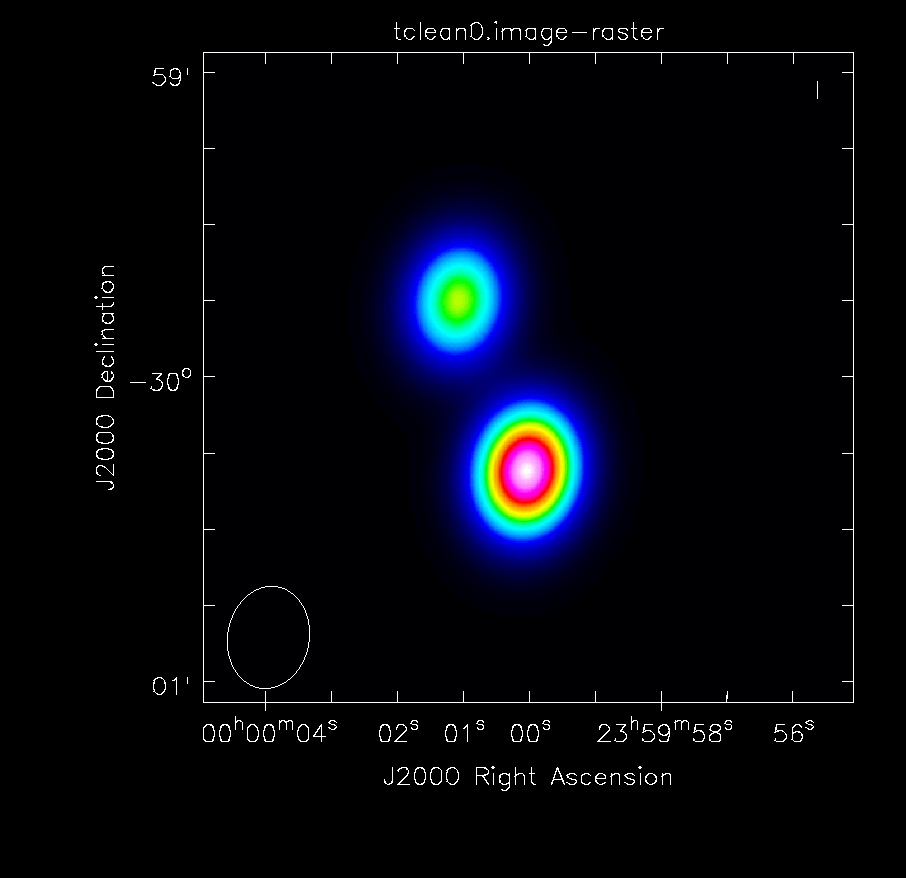
\includegraphics[height=3cm]{./chapters/01.intro/first.png}%
			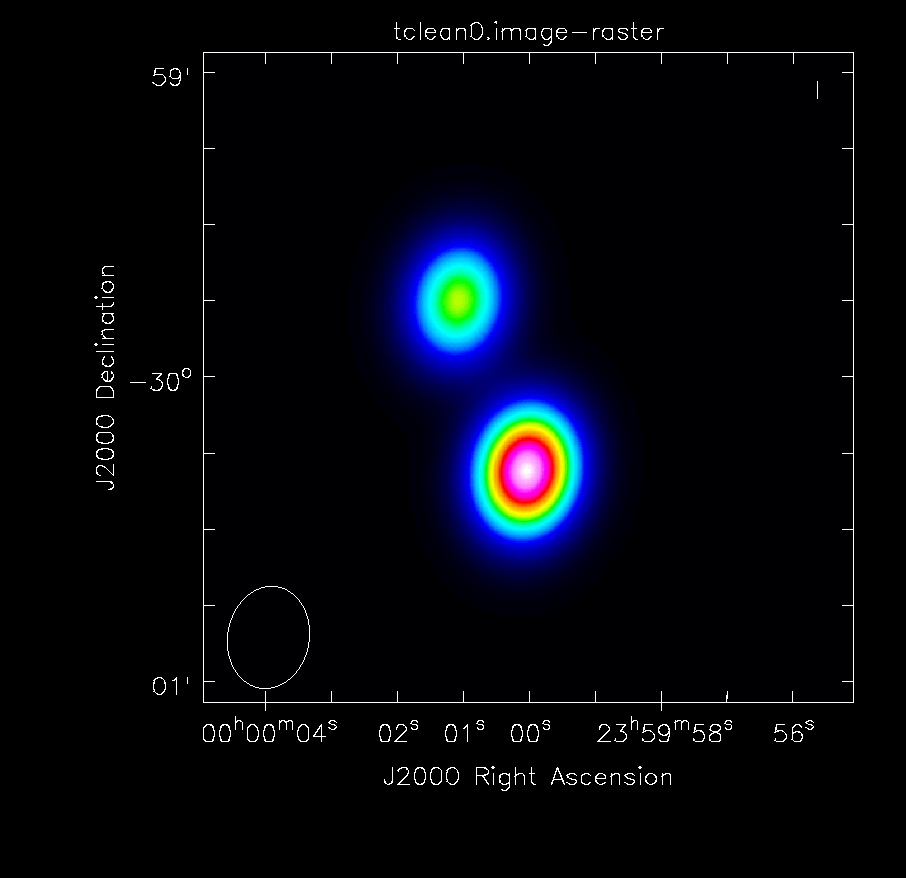
\includegraphics[height=3cm]{./chapters/01.intro/first.png}%
		}%
	}
	\setlength{\twosubht}{\ht\twosubbox}
	
	% typeset
	\centering
	\subcaptionbox{Measurements of the interferometer in the Fourier space.\label{intro0:inversefig:uvspace}}{%
		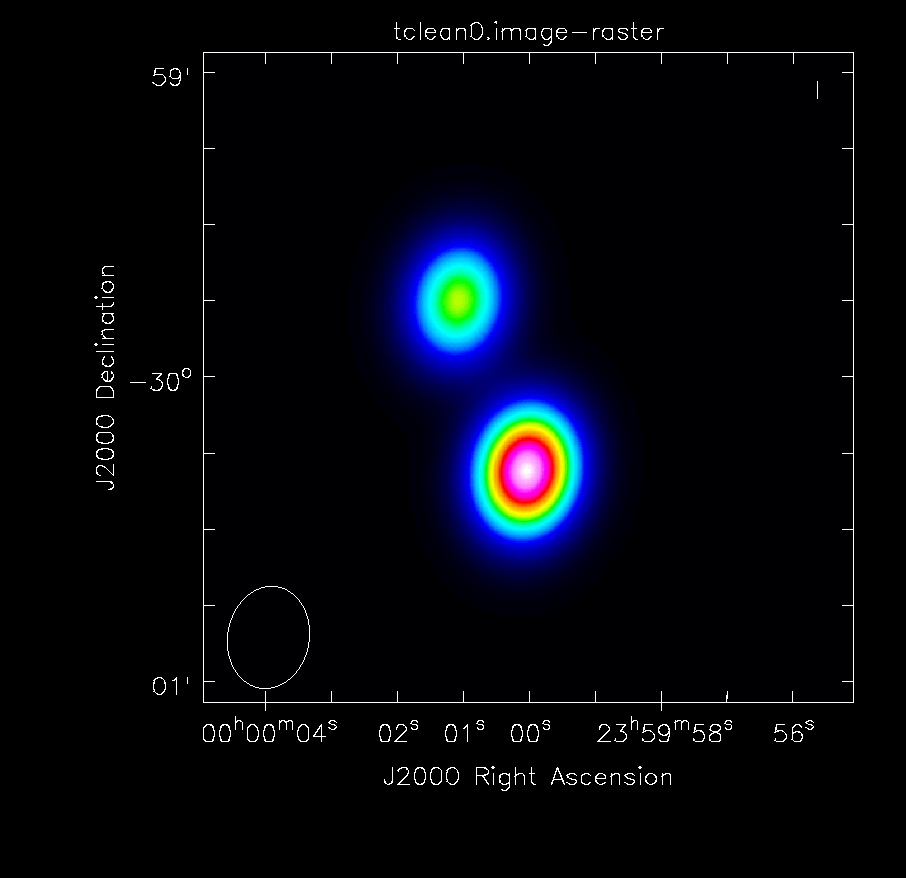
\includegraphics[height=\twosubht]{./chapters/01.intro/first.png}%
	}\quad
	\subcaptionbox{Observed image of the sky, showing two stars.\label{intro0:inversefig:reconstruction}}{%
		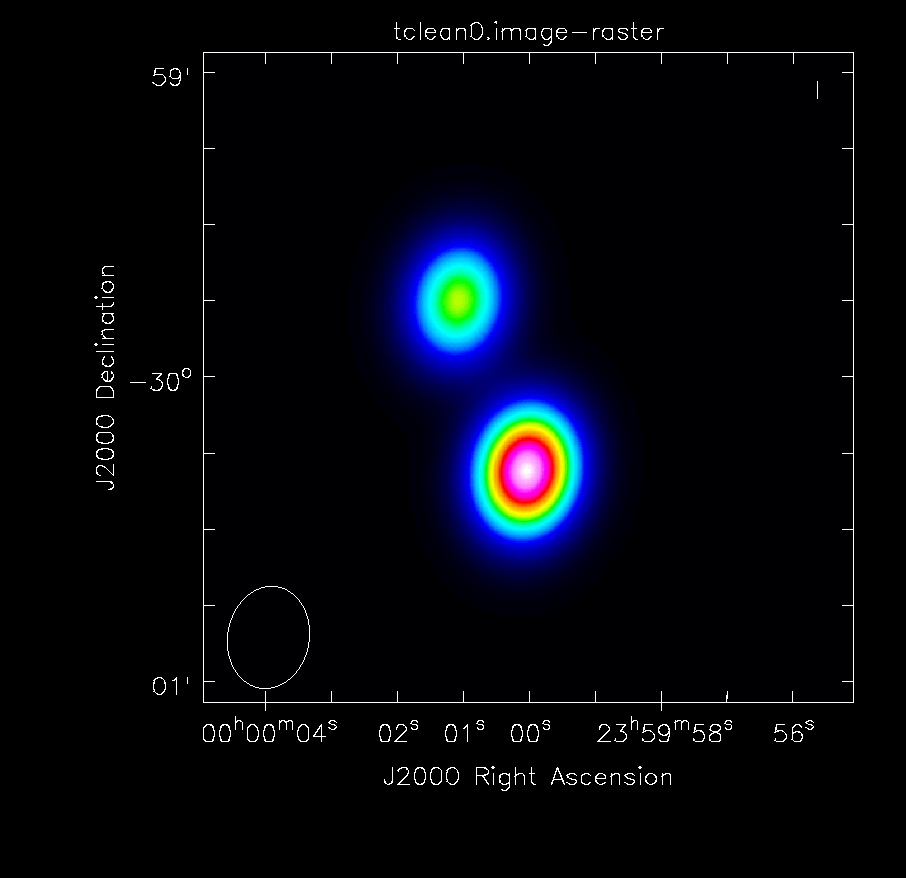
\includegraphics[height=\twosubht]{./chapters/01.intro/first.png}%
	}
	\caption{The image reconstruction problem, the observed image has to be reconstructed from the Fourier measurements.}\label{intro0:inversefig}
\end{figure}

In Astronomy, one goal is to find ever smaller objects in the sky. For this purpose, we build instruments with higher angular resolution. The instruments angular resolution depends on two factors: On the diameter of the antenna-dish or mirror, and on the observed wavelength. With longer wavelengths we need bigger dishes/mirrors to achieve a similar angular resolution. 

This is an issue for Radio Astronomy. The long radio wavelengths require huge dishes for a high angular resolution. Of course there is a practical limit on the antenna-dish diameter we can build. The famous Arecibo observatory is one of the largest single-dish radio telescopes with a diameter of 305 meters. Antennas with such a large diameter become difficult to steer accurately, let alone the construction costs. We have reached the practical limits of single-dish telescopes. If we require higher angular resolution, we need to look at another type of instrument: The radio interferometer. They use several smaller antennas together, acting like a single large dish. An interferometer can achieve angular resolutions which are comparable to dishes with a diameter of several kilometers.

But there are drawbacks: The interferometer does not measure the sky in pixels. It measures the amplitude and phase of Fourier components at a given $u$ and $v$ location\footnote{$u$ and $v$ are the axis in Fourier space}. The observed image has to be reconstructed from the measurements. The figure \ref{intro0:inversefig} shows an example of the image reconstruction problem. The figure \ref{intro0:inversefig:uvspace} shows the measurements in the Fourier space, and the figure \ref{intro0:inversefig:reconstruction} shows the observed image of the sky, with two stars close to each other. The image reconstruction has to find the observed image \ref{intro0:inversefig:reconstruction} from the measurements \ref{intro0:inversefig:uvspace}. 

At first glance, we might believe that the image reconstruction is trivial: The interferometer measures Fourier components, and efficient algorithms for the inverse Fourier transforms are well-known. However, two properties of the measured Fourier components make the image reconstruction difficult: The measurements are both noisy and incomplete.

The atmosphere of the earth is one source that introduces noise.. It adds noise to the amplitude and phase of each measured Fourier component. The atmosphere changes over time and can under the right circumstances introduce a high level of noise compared to the signal. The image reconstruction should be able to find the observed image from potentially very noisy Fourier measurements.

The interferometer measures an incomplete set of Fourier components note that the figure \ref{intro0:inversefig:uvspace} does not contain a noisy measurement of every non-zero Fourier component. There are Fourier components with non-zero amplitudes that the interferometer has not seen. The reconstruction algorithm has to find the observed image even though important Fourier components are missing from the measurements.

These two difficulties, the noise and the incomplete measurements make the image reconstruction an ill-posed inverse problem. There are many different images that fit the measurements, and from the measurements alone, we cannot decide which is the truly observed image. 

We cannot find the observed image, all we can do is find the most likely observed image. This is the what an image reconstruction algorithm produces: It uses prior knowledge about the image and finds the most likely observed image given the data. It uses a numerical optimization algorithm to find the optimal trade-off between being as close to the data, and being as consistent with the prior knowledge as possible.

The question that comes to mind is: How close are the most-likely image of the reconstruction algorithms to the observed image? The answer depends on the noise level in the measurements. On a low noise level, recently developed algorithms were shown to super-resolve the observed image\cite{dabbech2018cygnus, dabbech2015moresane}, to reconstruct the image above the accuracy limit of the instrument. However, not all algorithms perform equally well when the noise level in the measurements is high. Also, computing resources required for each algorithm can vary significantly. In short, a reconstruction algorithm in Radio Astronomy has three opposing goals:
\begin{enumerate}
	\item Produce a reconstruction with the highest possible resolution from the measurements.
	\item Robust against even heavy noise in the measurements.
	\item Use as few computing resources as possible.
\end{enumerate}

T

There is no reconstruction algorithm that has the optimal trade-off between all three goals. It is an active field of research.

To complicate things further, newly constructed radio interferometers pose the reconstruction problem on a big data scale. The recently finished MeerKAT radio interferometer produces roughly 80 million Fourier measurements each second.
We need to distribute the image reconstruction. This is an active field of research.
Research into how we can perform the image reconstruction in a

The ideal reconstruction algorithm not only achieves all three opposing goals, but is also distributable in a super-computer environment, preferably on the GPU. This is a tall order. So far, the go-to reconstruction algorithm CLEAN was performing its numerical optimization on a single machine. The new data volume raises the need for distributed and GPU-Accelerated optimization algorithms.

We explore coordinate Descent.

This Project focuses on the third point, distributed image reconstruction with real-world meerkat observations
Received from SARAO for the purpose of algorithmic validation.

\newpage
\section{Introduction to radio interferometric imaging}\label{radio}
%This Section gives an introduction to radio interferometric imaging. We introduce how the interferometer measures visibilities, what problems arise and how reconstruction algorithms solve them. 

A radio interferometer consists of several antennas. Each antenna pair measures a visibility in Fourier space. Each measurement consists of an amplitude and phase at a location at a $u$ and $v$  location. The distance between the antennas, which we call the baseline, defines what point in the Fourier space gets sampled. The Figure \ref{radio:sampling:ants} shows the antenna layout of the MeerKAT radio interferometer, and the Figure \ref{radio:sampling:pattern} shows the measurement points in Fourier space. Short baselines sample points close to the origin, and contain the low-frequency Fourier components. They contain information about large areas of the images. Longer baselines measure points further away from the origin. They sample the high-frequency Fourier components. They contain information about edges, and other small structures in the image.


\begin{figure}[!h]
	\centering
	\begin{subfigure}[b]{0.49\linewidth}
		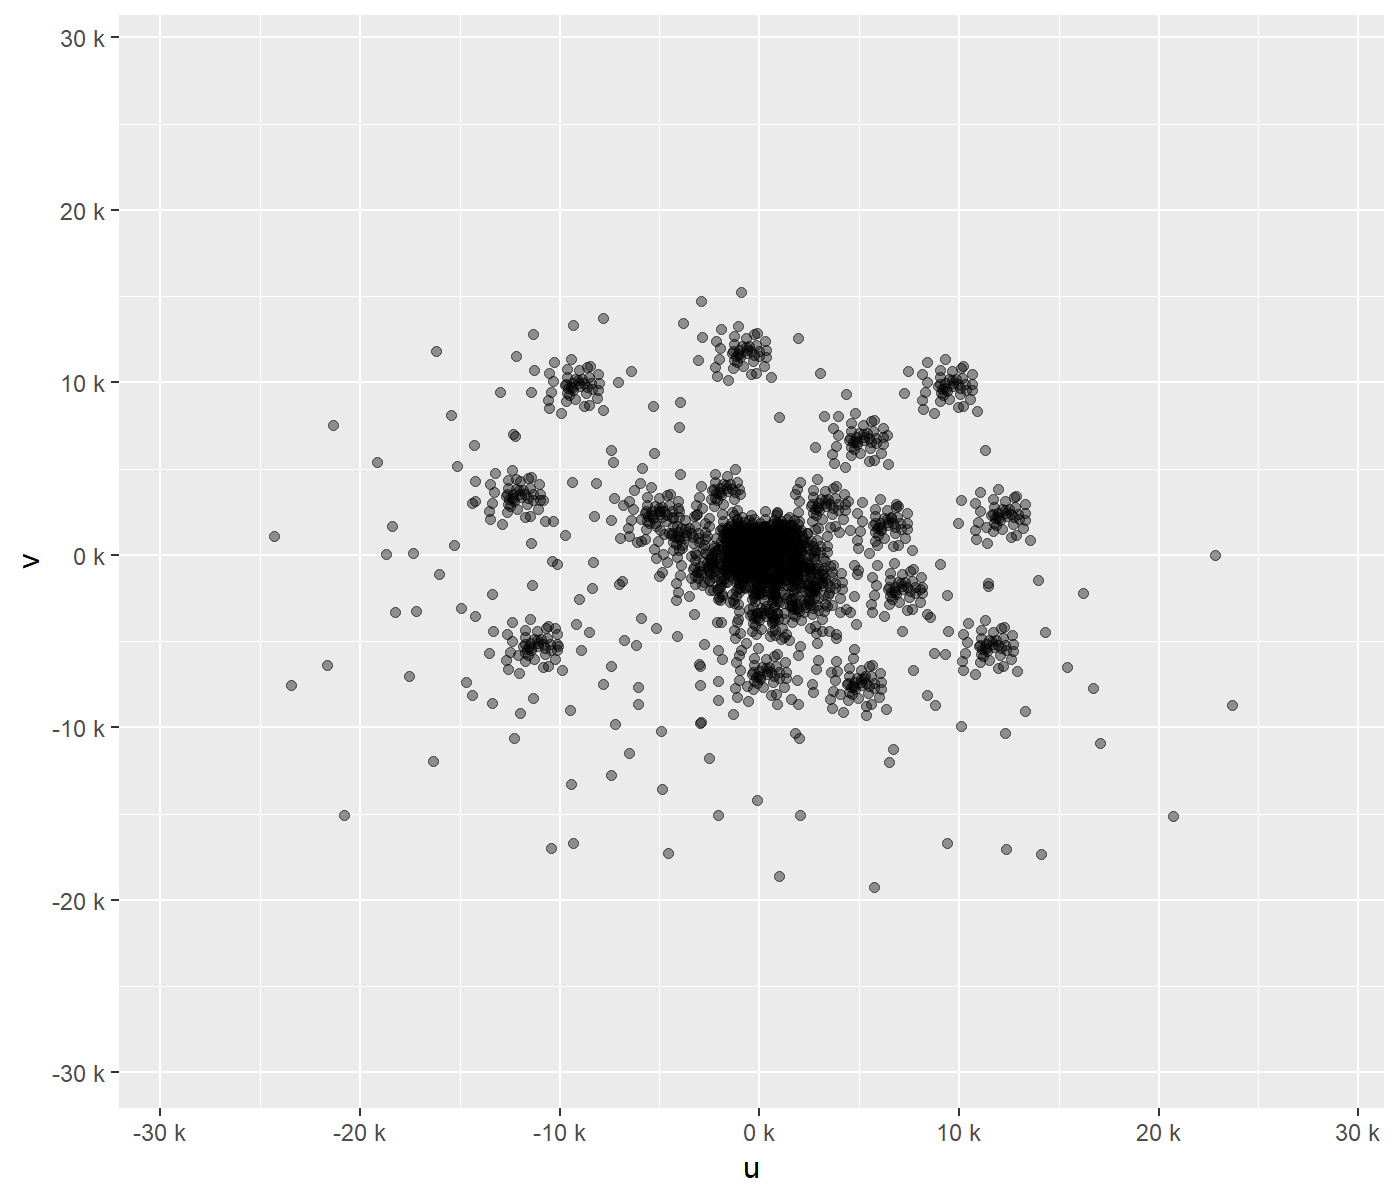
\includegraphics[width=\linewidth]{./chapters/01.intro/aperture/snapshot.png}
		\caption{Antenna layout.}
		\label{radio:sampling:ants}
	\end{subfigure}
	\begin{subfigure}[b]{0.49\linewidth}
		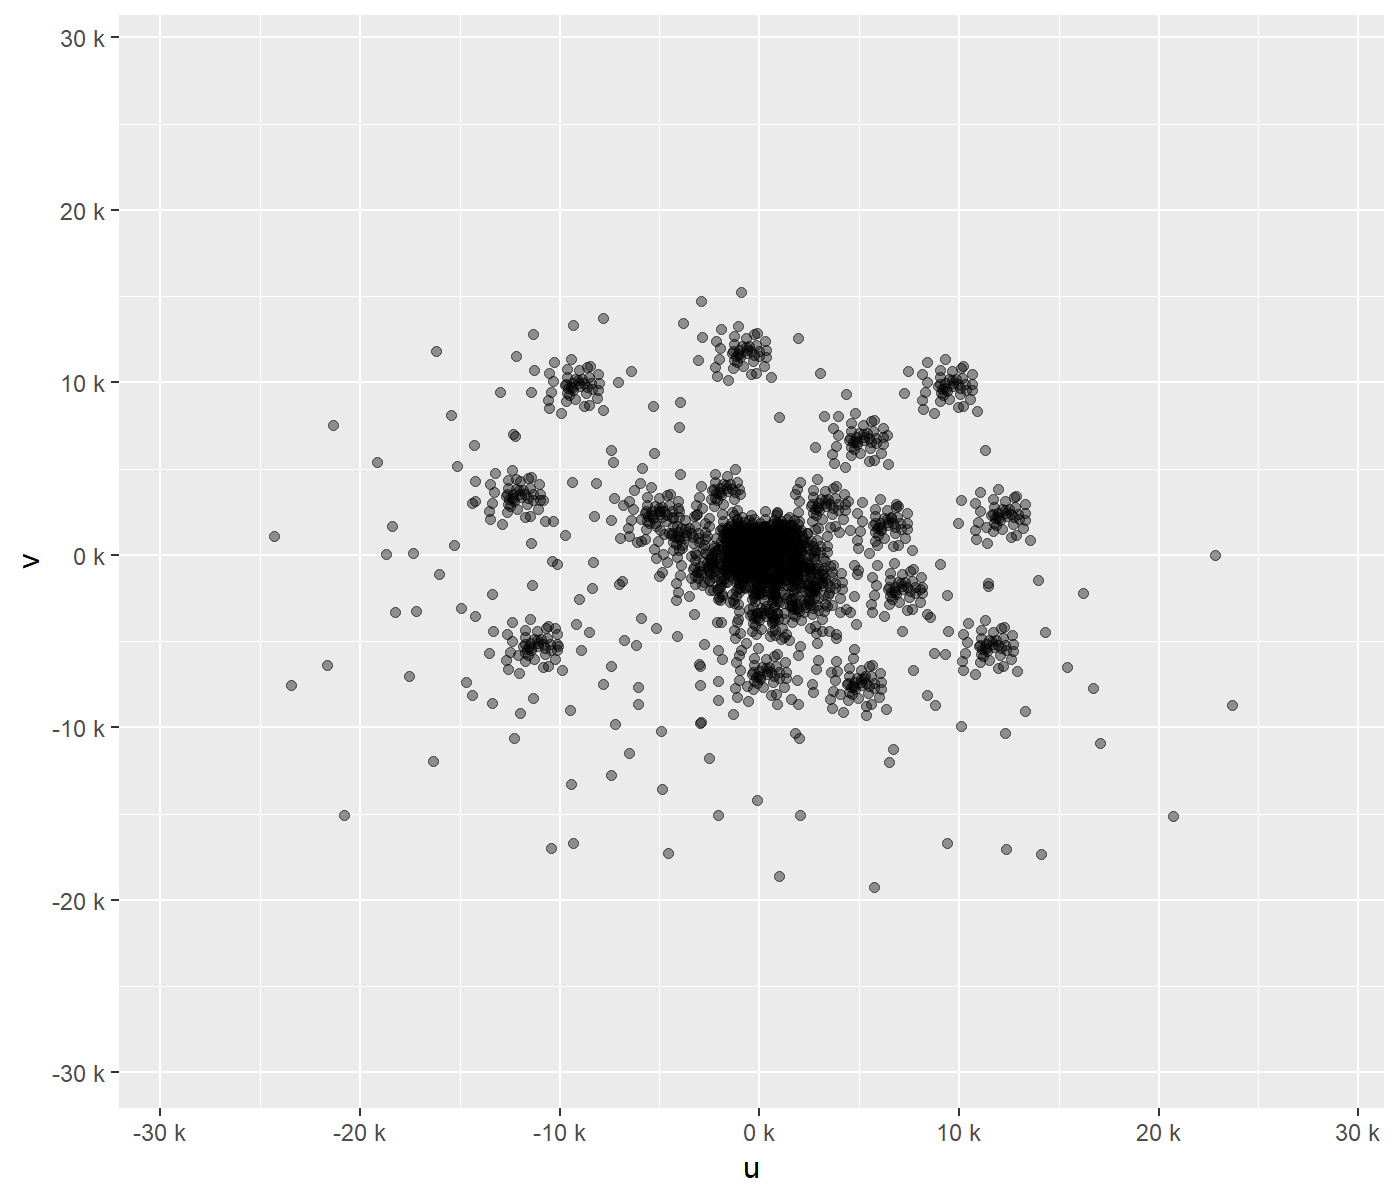
\includegraphics[width=\linewidth]{./chapters/01.intro/aperture/snapshot.png}
		\caption{Visibility sampling pattern.}
		\label{radio:sampling:pattern}
	\end{subfigure}
	\\
	\begin{subfigure}[b]{0.49\linewidth}
		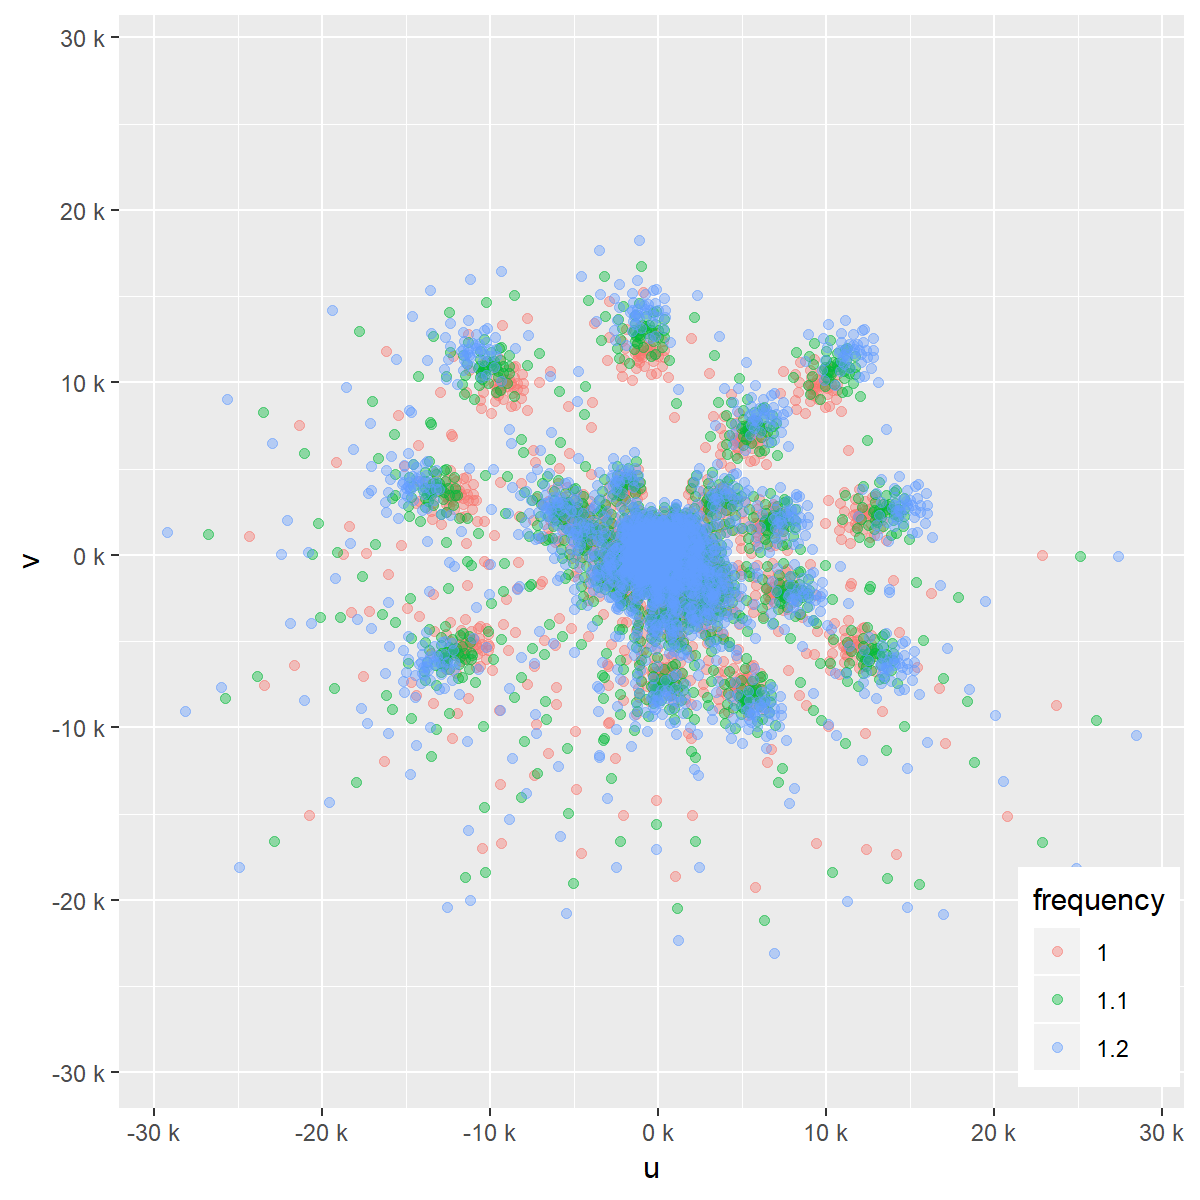
\includegraphics[width=\linewidth]{./chapters/01.intro/aperture/frequencies.png}
		\caption{Visibilities added from multiple channels.}
		\label{radio:sampling:freq}
	\end{subfigure}
	\begin{subfigure}[b]{0.49\linewidth}
		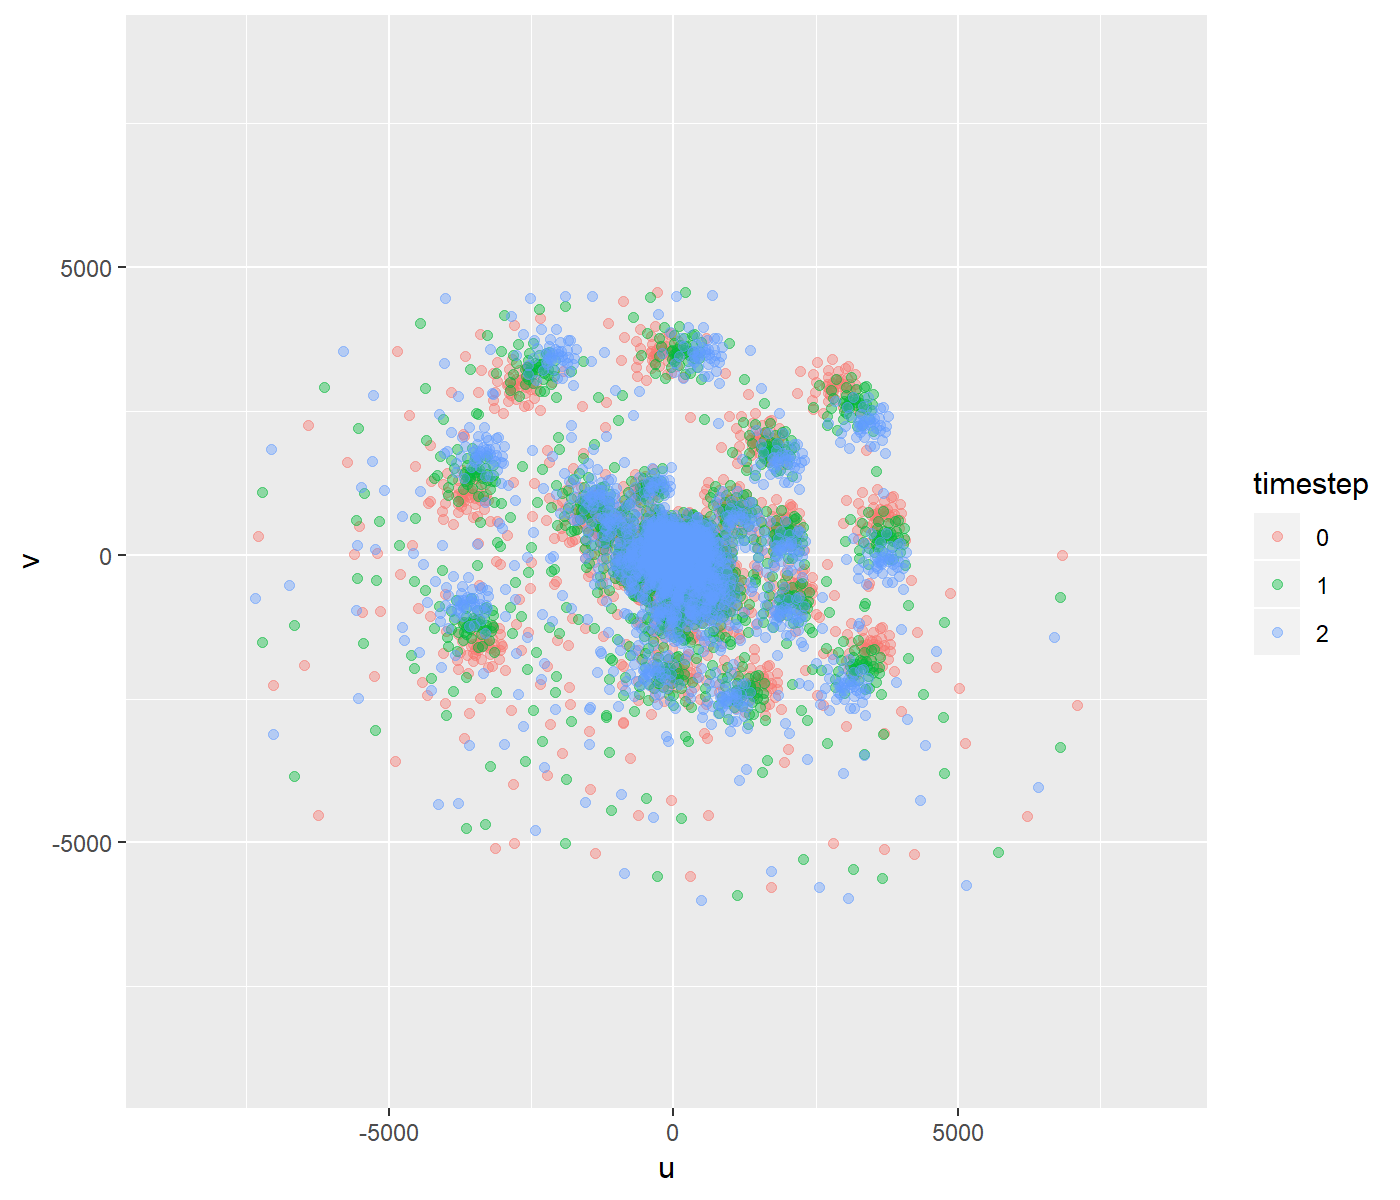
\includegraphics[width=\linewidth]{./chapters/01.intro/aperture/timesteps.png}
		\caption{Visibilities added from multiple timesteps.}
		\label{radio:sampling:time}
	\end{subfigure}
	
	\caption{Sampling regime of the MeerKAT radio interferometer.}
	\label{intro:sampling}
\end{figure}

The sampling pattern of the MeerKAT interferometer is not uniform in the Fourier space. We have areas which are densely sampled, and areas which are sparsely sampled. Note that we only have a few samples of the high-frequency Fourier components. We are missing measurements from a large portion of the Fourier space.

Radio interferometers use two "tricks" to measure more points in the Fourier space. Radio interferometers measure the sky in different radio channels simultaneously. We can add the visibility measurements from different channels together, shown in Figure \ref{radio:sampling:freq}. Each channel measures the Fourier space using the same pattern, but scaled by the radio frequency. 

The second trick is to use the earth's rotation to sample different points in the Fourier space. The earth's rotation also rotates the sampling pattern in Fourier space, shown in Figure \ref{radio:sampling:time}, and we can sample the Fourier space at new locations.

The MeerKAT radio interferometer measures 2016 visibilities, for each channel, at each timestep. It has 20 thousand radio channels. The time resolution can be as low as half a second. This results in roughly 80 million visibility measurements per second. In radio astronomy, we want to reconstruct several hours worth of visibility measurements. 
%GB and TB of data

\begin{figure}[htp]
	% preliminary
	\sbox\twosubbox{%
		\resizebox{\dimexpr.9\textwidth-1em}{!}{%
			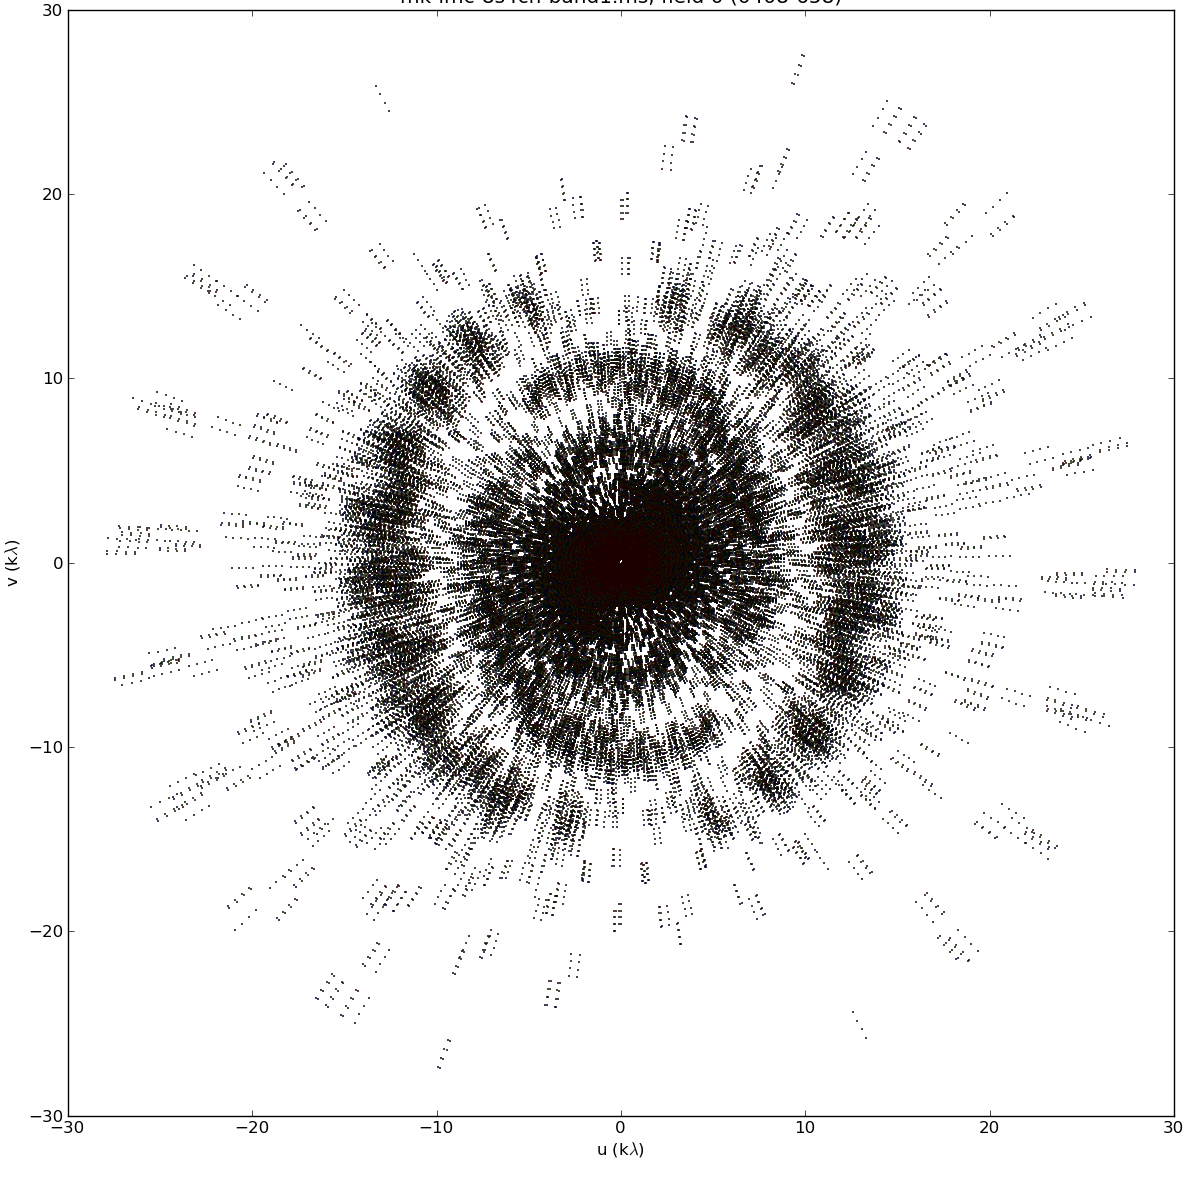
\includegraphics[height=3cm]{./chapters/01.intro/meerkat_uv2.png}%
			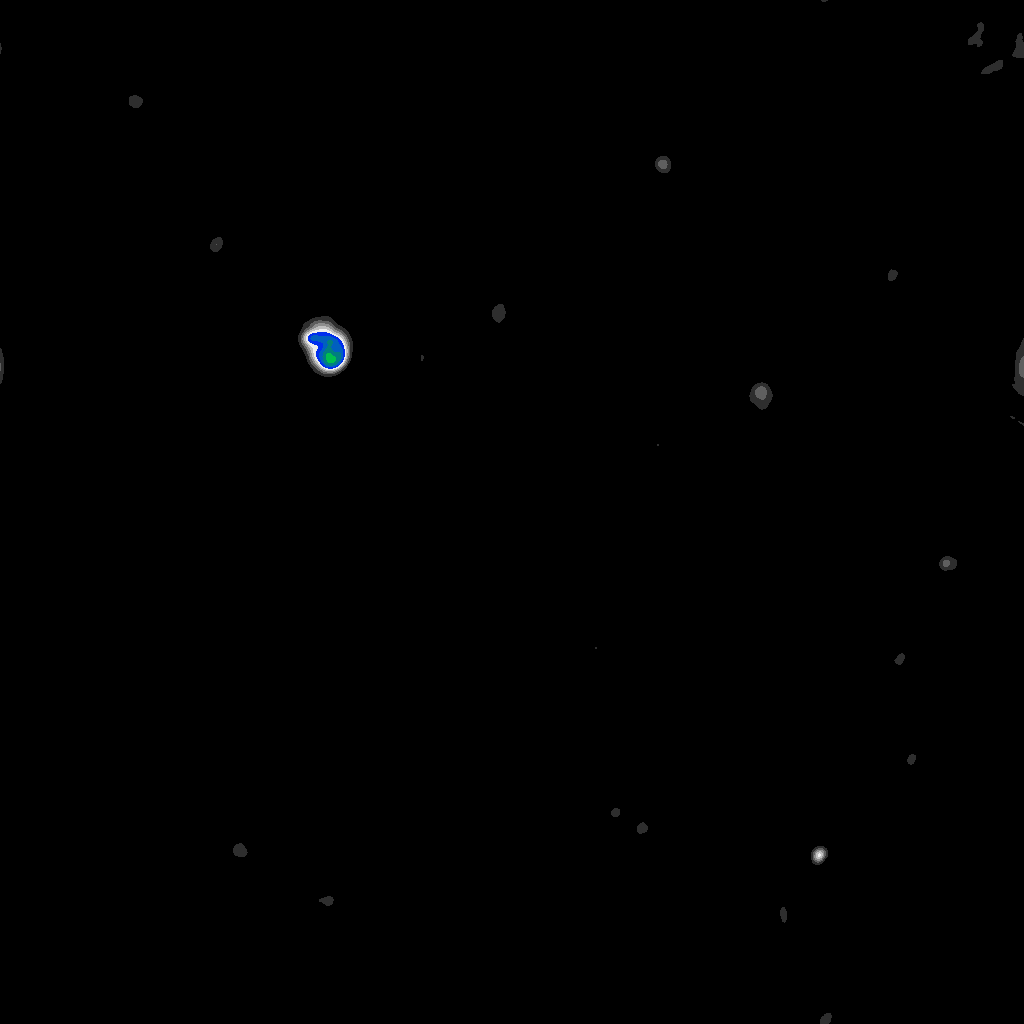
\includegraphics[height=3cm]{./chapters/01.intro/mk2/clean.png}%
		}%
	}
	\setlength{\twosubht}{\ht\twosubbox}
	
	% typeset
	\centering
	\subcaptionbox{Real-world visibilities combined from different channesl and timesteps.\label{intro:inversefig:uvspace}}{%
		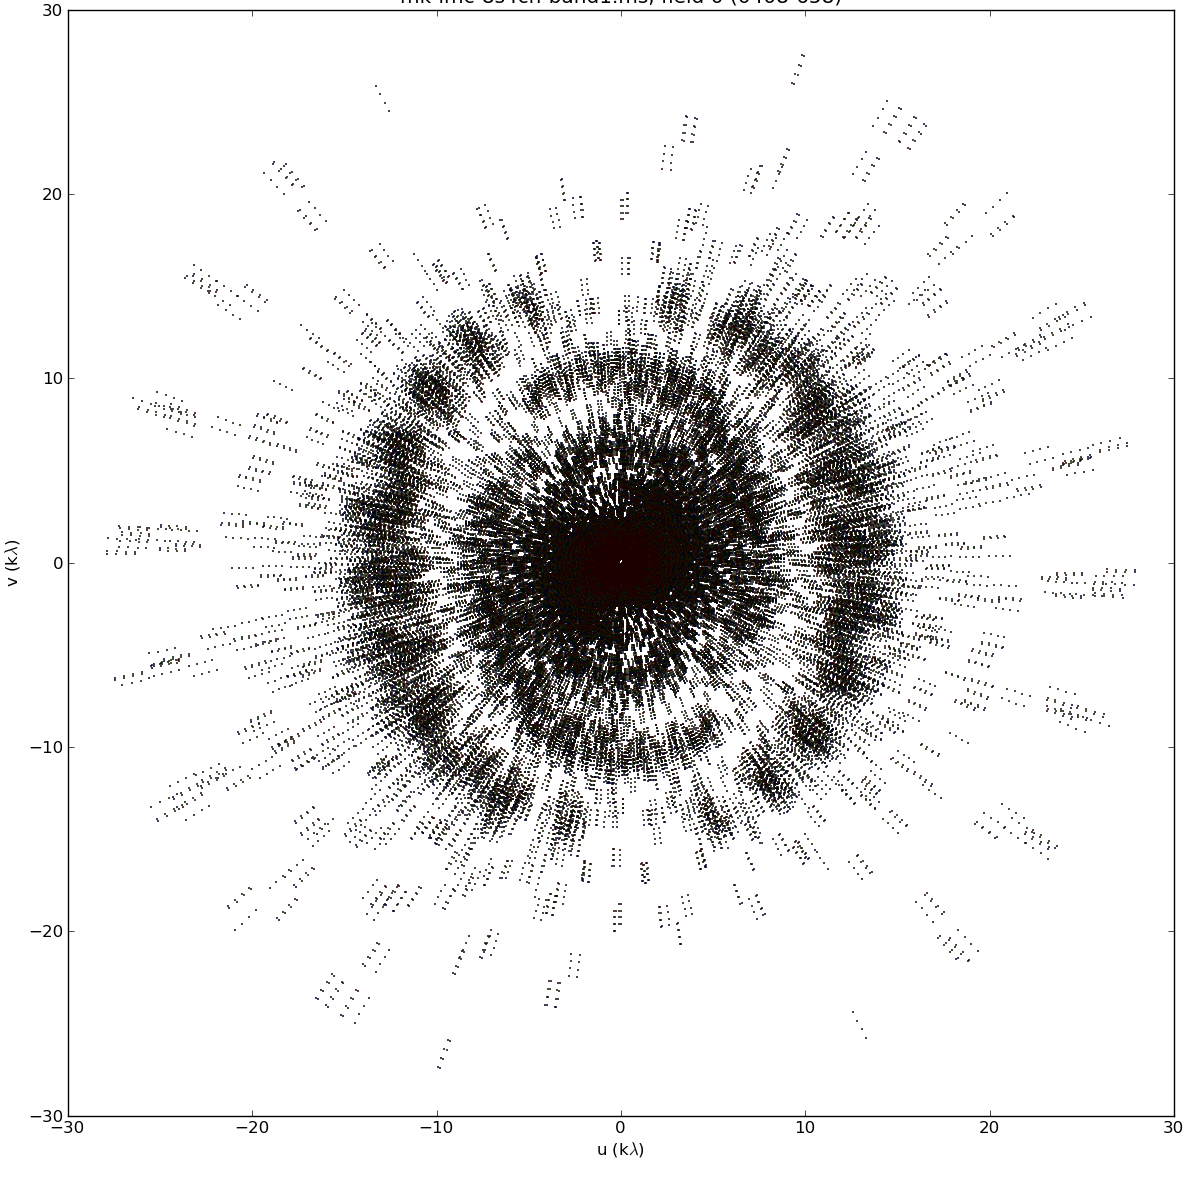
\includegraphics[height=\twosubht]{./chapters/01.intro/meerkat_uv2.png}%
	}\quad
	\subcaptionbox{Reconstruction of the visibility measurements.\label{intro:inversefig:reconstruction}}{%
		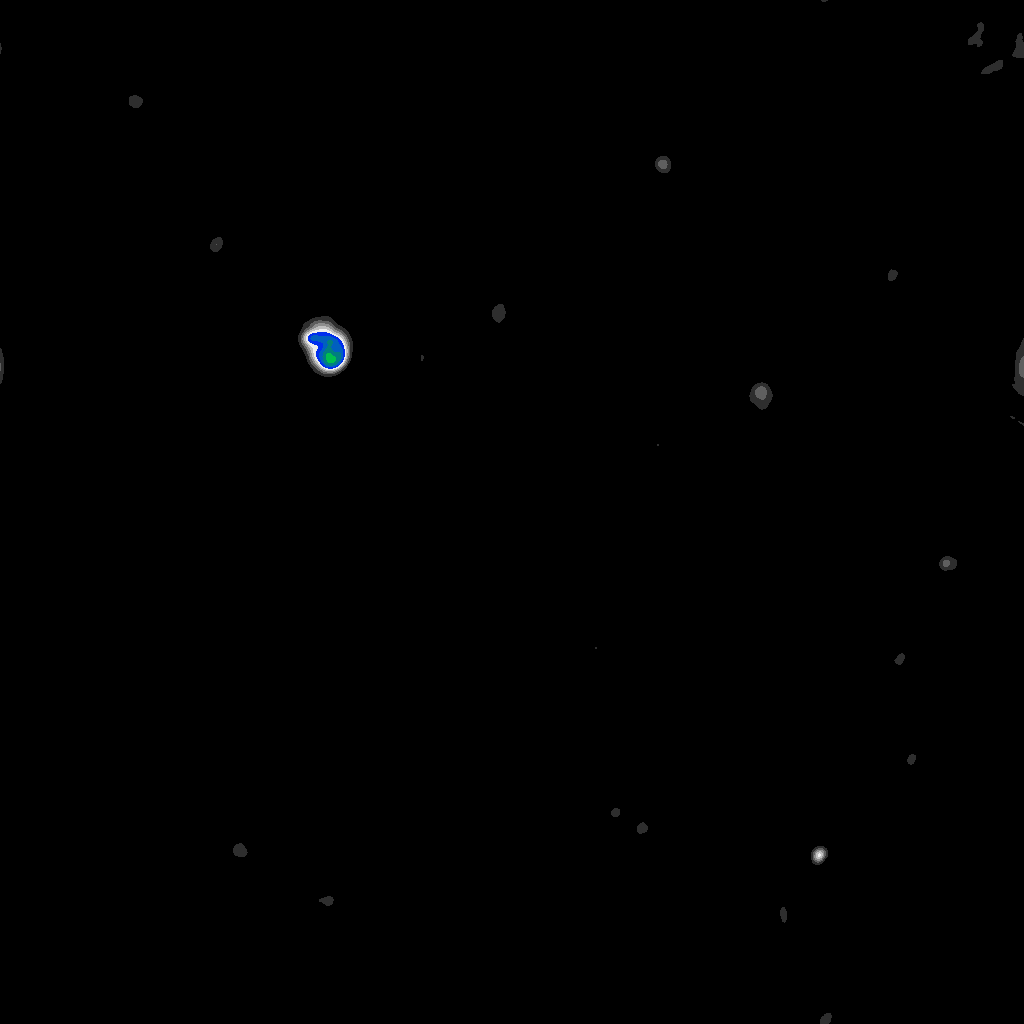
\includegraphics[height=\twosubht]{./chapters/01.intro/mk2/clean.png}%
	}
	\caption{Example of an image reconstruction for Fourier measurements of the MeerKAT radio interferometer}\label{intro:inversefig}
\end{figure}

A lot of visibility measurements. The Figure \ref{intro:inversefig:uvspace} shows a fraction of the visibility samples. 
The measurements from radio interferometers contain a large number of visibilities. The Figure  \ref{intro:inversefig:uvspace} shows the samples in Fourier space for a real world observation. The visibilities are combined from multiple channels and multiple timesteps. Although we have a large number of visibilities, we still have areas of the Fourier space without a sample. Although we have a large number of samples, the visibilities are still an incomplete. From the measurements alone, we cannot reconstruct the image shown in Figure \ref{intro:inversefig:uvspace}.

This is known as an ill-posed inverse problem in the literature. A problem is considered ill-posed when:
\begin{enumerate}
	\item No solution exists.
	\item There are solutions, but no unique solution exists.
	\item The solution behaviour does not change continuously with the initial condition (For example: a small change in the measurements lead to a very different reconstructed image).
\end{enumerate}
Image reconstruction for radio interferometer is an inverse problem, because we want to find the image which the interferometer observed in Fourier space. It is ill-posed in general, because there are many different images fitting the measurements.

Note that we can reduce the resolution of the reconstructed image until the problem becomes well-posed. The Nyquist-Shannon sampling theorem states the case of radio interferometers: The highest highest Fourier-frequency we measure should be more than twice the highest frequency in the image. The center of the Fourier space in Figure \ref{intro:inversefig:uvspace} is densely sampled. We can reconstruct a low-resolution image that only needs the information from the densely sampled center, and does not need the missing high-frequency Fourier components.

However, this would reduce the effective resolution of the reconstruction. We can solve the ill-posed inverse problem and retrieve the observed image at a higher resolution than possible with the Nyquist-Shannon sampling theorem. We solve the ill-posed inverse problem by including prior information about the observed image. This is known as the Compressed Sensing sampling theorem. We use numerical optimization algorithms to find the most likely image, which is consistent with the measurements and consistent with our prior information. The Compressed Sensing sampling theorem gives us theoretical guarantees that, under the right conditions, the most likely image is equal to the observed image.

%In Section \ref{intro2:ill-posed}, we introduce the Compressed Sensing sampling theorem and show how it works in the case of radio interferometric image reconstruction. The Section \ref{intro2:rec} shows how we can use the theory to create a reconstruction algorithm in practice. But first, we dive deeper into the odds and ends of radio interferometry. 



\subsection{The theory of Compressed Sensing}\label{intro2:ill-posed}

T

So far, we discussed how the interferometer measures in Fourier space, and we wish to find the observed image that matches the measurements. In other words, we wish to find a solution to a system of linear equation \eqref{intro2:ill-posed:linear}, where $V$ are the measurements, $x$ is the observed image and $F$ is the Fourier transform matrix. We also discussed that $F$ can be complicated in practice, but is still essentially a linear operator. Meaning we know how the inverse Fourier transform matrix $F^{-1}$, and the question arises: Why can't we solve the equations \eqref{intro2:ill-posed:linear} by calculating the inverse Fourier transform? Or, why does $x = F^{-1} V$ not lead to the observed image?

\begin{equation}\label{intro2:ill-posed:linear}
\underset{x}{solve}\quad V - Fx = 0
\end{equation}

The answer is, the equations \eqref{intro2:ill-posed:linear} do not have a unique solution, which makes the problem ill-posed. The problem is considered ill-posed when it has one of the following properties:
\begin{enumerate}
	\item No solution exists.
	\item There are solutions, but no unique solution exists.
	\item The solution behaviour does not change continuously with the initial condition (For example: a small change in the measurements lead to a very different reconstructed image).
\end{enumerate}
From linear algebra, we know that an under-determined system of linear equations, i.e. when \eqref{intro2:ill-posed:linear} has more pixels than visibility measurements, then the problem is under-determined and there may be a potentially infinite number of solutions to the system. Under-determined systems arise in many similar fields, as for example in X-Ray imaging of the sun\cite{felix2017compressed}. However, radio interferometers measure a large number of visibilities. We generally have more visibilities than pixels. This means the image reconstruction problem \eqref{intro2:ill-posed:linear} for radio interferometers is actually over-determined.

From linear algebra, we know that an over-determined system either has one or zero solutions. At first glance it may be counter-intuitive why there are many possible solutions to \eqref{intro2:ill-posed:linear} for radio interferometers. The reason why lies in two properties of the measurements: They are noisy and incomplete.

The radio interferometer measures noisy visibilities, meaning each amplitude and phase of a measurement is influenced by an unknown noise factor. Finding a reconstructed image is the same as finding the de-noised versions of the visibility measurements. This alone would make the problem ill-posed, but the visibilities actually have a second property that makes them ill-posed: incompleteness.

When we look back at figure \ref{intro:inversefig:uvspace}, it is clear to see that the interferometer does not sample the visibilities in a uniform way. There are regions with a high sample density. The density decreases when we move further away from the center. The higher frequency visibilities get fewer and fewer samples. This means we are missing data for crucial measurements for the reconstruction.

Also note that the question whether the measurements are incomplete essentially comes down to the image resolution of the reconstruction: Since we are missing high-frequency measurements and we can choose the resolution of the image, we can also reduce the resolution of the reconstructed image until the missing frequencies become negligible. However, if we can solve the ill-posed inverse problem, we can reconstruct an image at a higher resolution from the same measurements. The question is how do we solve the ill-posed inverse problem?

\subsubsection{Adding a regularization} \label{intro:linear:regularization}
For ill-posed inverse problems, there are two viewpoints for the same idea. From the viewpoint of optimization, we can solve the ill-posed image reconstruction problem \eqref{intro:linear:linear} by adding a regularization. The regularization creates a system of linear equations with a unique solution. From the viewpoint of Bayesian Statistics, we include prior knowledge about the image, and therefore search the most likely image given the measurements. For this project, both terms describe the same idea and we use regularization and prior interchangeably. We know that the reconstructed image from radio interferometers contain a mixture of stars (point sources located in a single pixel) and extended emissions like hydrogen clouds. By adding this prior knowledge to the reconstruction problem, we can find the most likely image given the measurements. As we will see, under the right prior, we can create a reconstruction algorithm that is almost guaranteed to find the truly observed image in theory.

There are different ways to include regularization in the reconstruction problem. In this project, we use the following method: We cast the image reconstruction problem into an optimization objective consisting of a data fidelity term and a regularization term. A reconstruction algorithm therefore consists of an optimization objective, a prior function and an optimization algorithm.

\begin{equation}\label{intro:linear:compressed}
\underset{x}{minimize} \: \left \| V - Fx \right \|_2^2 + \lambda P(x)
\end{equation}

The objective \eqref{intro:linear:compressed} has a data term $\left \| V - Fx \right \|_2^2$, which forces the most likely image to be as close to the measurements as possible, and the regularization term $P(x)$, which penalizes unlikely images according to our prior function. The parameter $\lambda$ represents how much we penalize unlikely images and by extend, much noise we expect in the reconstruction. The parameter $\lambda$ is either left to the user to define, can be estimated from the data \cite{miller1970least}. 

The prior function $P()$ represents our prior knowledge about the image. It assigns a high penalty for unlikely images. In in radio interferometric image reconstructions tend to use similar prior functions as for image de-noising applications. Such as: Total Variation ($\left \| \triangledown x \right \|_1$) \cite{wiaux2009compressed}, L2 ($\left \|x \right \|_2$) \cite{ferrari2014distributed} or the L1 norm in a wavelet space ($\left \|\Psi x \right \|_1$) \cite{girard2015sparse}.

Finally, an optimization algorithm is necessary which can optimize the objective function \eqref{intro:linear:compressed} with the chosen prior function $P()$. Typical choices for optimization algorithms in image reconstructions are Interior Point Methods like Simplex, Matching Pursuit \cite{hogbom1974aperture} and ADMM\cite{carrillo2014purify}. 

A reconstruction algorithm for radio astronomy consists of an optimization objective, a prior function and an optimization algorithm. It is a three dimensional design space. Not every prior is suitable for every optimization algorithm. The choice of optimization objective influences both what prior and what optimization algorithm we can use. Although there are a different choices for the optimization objective, we limit ourselves to the objective \eqref{intro:linear:compressed} and explore how we can distribute the reconstruction problem.

The last question that remains is, how close are the most likely image, under a given prior, to the truly observed one? Remember that the Nyquist-Shannon sampling theorem states that our uniform sampling frequency needs to be larger than twice the highest frequency in a band-limited signal\footnote{For example: if we want to record human voices with the highest frequency of 20 kHz, Nyquist-Shannon states our uniform sampling frequency has to be larger than 40 kHz to guarantee exact reconstruction}, and then the theorem guarantees exact reconstruction. For radio astronomy, we do not have uniformly sampled visibilities, and although we have a large number of samples, we are missing crucial parts of the Fourier space. Luckily, there is another sampling theorem that, under certain assumptions, guarantees exact reconstruction for the case of radio interferometers: The theory of compressed sensing.

\subsubsection{Compressive sampling of the sky}
For the sake of demonstration, let us assume the radio interferometer observes a patch of sky containing ten stars. It measures an incomplete set of random Fourier components of the ten stars, and we would like to reconstruct an image of size $256^2$ pixels. The emissions from stars are concentrated into a single pixel. For compressive sampling, we need to know an space in which our reconstructed image is sparse, and we need to take measurements in a different, incoherent space.

Our reconstructed image contains only zero pixels except at the ten locations of the stars, meaning the image space for this patch of the sky is already sparse. In this case, we do not need any additional sparse space like wavelets. We can reconstruct directly in the sparse image space, and we have the first requirement met for compressive sampling. 

The next requirement is that the measurement and reconstruction space (which is the image in this example), are as incoherent as possible. 

Yes, incoherence.
\begin{equation}\label{intro:linear:compressed2}
\underset{x}{minimize} \: \left \| V - Fx \right \|_2^2 + \lambda \left \| x \right \|_1
\end{equation}


Intuitively, the number of samples depend on the information content, not on the bandwidth. thi


At what point are we guaranteed? The matrix $A$ needs to fullfil the Restricted Isometry Porperty (RIP) \cite{candes2006robust,donoho2006compressed}.
Approximately orthonormal on sparse signals. (If we randomly choose ten columns of $F$, how much do they correlate. We want as little correlation as possible.)
Calculate the RIP is NP-hard\cite{tillmann2013computational}. Approximations are also difficult to compute\cite{natarajan2014computational}.
So we can only talk about how likely a given matrix fullfils the RIP. Matrix where each element is sampled from a random Gaussian distributîon has the highest change.

Random samples in the Fourier space also have a high chance to fulfill the RIP \cite{haviv2017restricted}.

Not possible for Radio interferometers, because they sample in the Fourier space. Not random.

There are also extended emissions, clouds etc. Resulting in a lot of non-zero pixels. There may be better sparse spaces for radio astronomy.

But also RIP may be too strict. Exact reconstruction can also work under less strict conditions\cite{candes2011probabilistic} active field of research.

\subsubsection{Reconstruction guarantees in the real world}

What does this all mean for image reconstruction?
For us, we design reconstruction algorithms and cannot influence the matrix $F$. We do not know if it actually 

The theory of compressed sensing gives us a framework. There is a data modelling task, and a task for finding efficient algorithms.

So there is a data modelling task in finding a good sparse prior.
We also do not know the proper sparse space in which radio interferometric images. We know several spaces, Curvelets \cite{starck2003astronomical} Starlets \cite{starck2015starlet}, Daubechies wavelets \cite{carrillo2012sparsity}. As of the time of writing, it is currently unknown which leads to the best reconstruction.
We can also learn dictionaries.

The task for efficient algorithms is finding the best way to optimize the objective with a given prior on real hardware. Fast convergence. Also difficult, because in practice the choice of prior can also influence convergence.


Compressed sensing based reconstruction algorithm. In radio astronomy.



\subsection{Noise, approximations and other difficulties in radio interferometry}
We give a short introduction into how the electromagnetic wave gets measured by the interferometer, turned into visibilities and finally processed into an image. Figure \ref{intro:system} shows a radio source and its electro-magnetic (em) wave arriving at the antennas of the interferometer. It then shows the three processes involved to arrive at an image: Correlation, calibration and image reconstruction.
	
\begin{figure}[h]
	\centering
	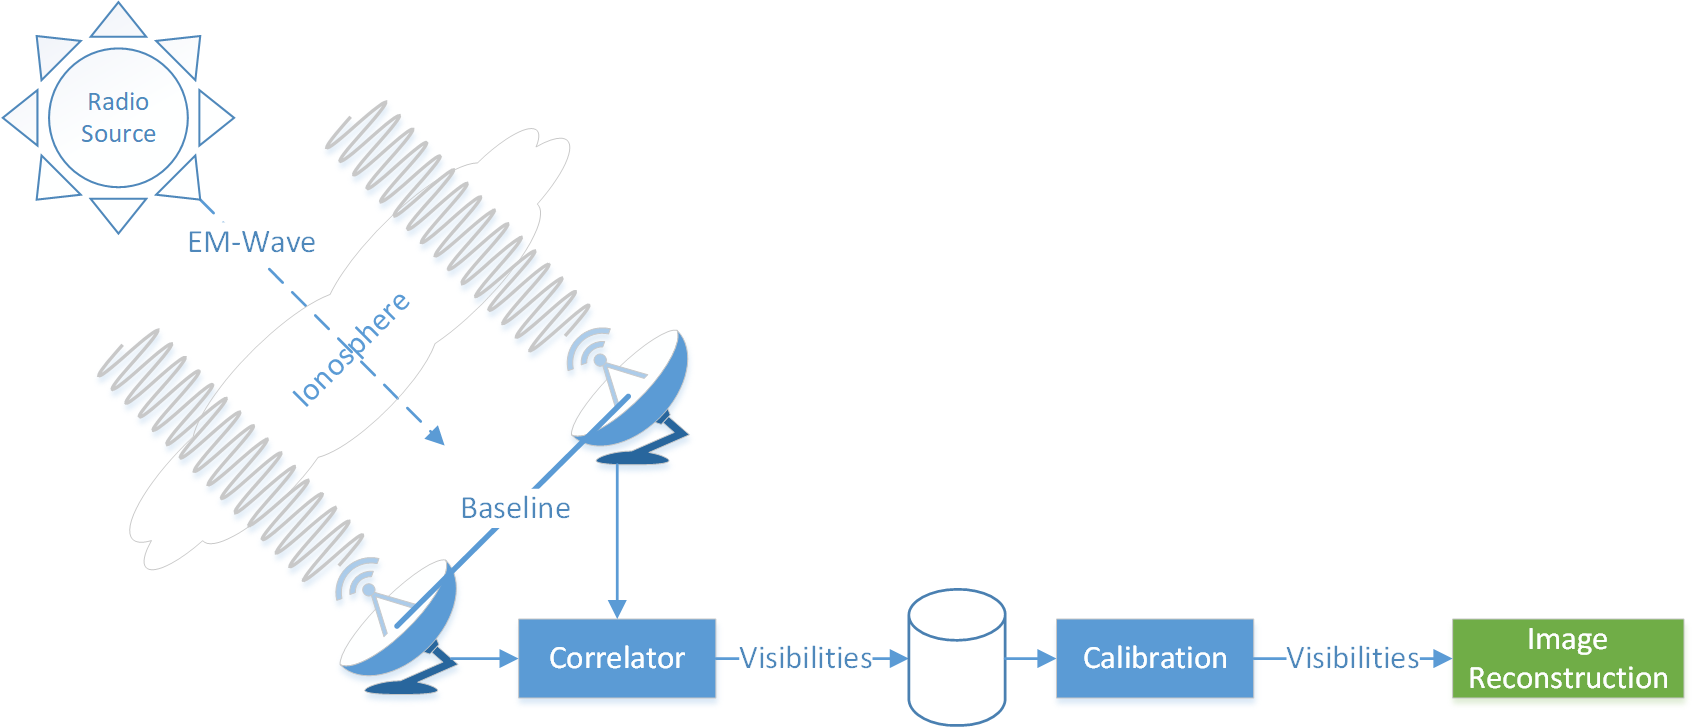
\includegraphics[width=0.80\linewidth]{./chapters/01.intro/system.png}
	\caption{Radio interferometer system}
	\label{intro:system}
\end{figure}

First, we have a source in the sky that is emitting em-waves in the radio frequency. The waves travel to earth, through the earth's ionosphere and finally to our interferometer. Along its path, the e-m waves may get distorted from various sources. For example, it may receive a phase shift by the ionosphere.

Then, the em-wave arrives at our interferometer. We call each antenna pair a baseline. Each baseline will end up measuring a single visibility. The distance between the antennas and their orientation to the em-wave will determine where we sample the $uv$-plane. Short baselines measure the $uv$-plane close at the origin, while long baselines sample the $uv$-space further away from the origin. Remember that the samples away from the $uv$-origin contain the information about edges and other details of our image. With a longer baseline the interferometer measures more highly resolved details, regardless of the antenna dish-diameter\footnote{Remember that this is the reason why we build radio interferometers. We do not need impossibly large dish diameters for a high angular resolution. We just need large distances between smaller antennas.}. The figure \ref{intro:system} shows the em-wave arriving at a single baseline of the interferometer. Each antenna picks up its version of the em-wave and transfers it to the correlator.

The correlator then takes the feed of each antenna and correlates the signals, which results in the amplitude and phase of the visibility component. Amplitude and phase for each visibility are measured for a short time range (i.e. fractions of a second up to several seconds). At this point, the visibilities are saved to disk for further processing. The radio interferometer produces a visibility measurement for each baseline, for each time range, for each frequency channel of the instrument. Because a single observation can take up to several hours, measured with several thousand frequency channels, radio interferometers produce an almost arbitrary large number of visibilities.

Calibration

Image Reconstruction

%Calibration. Effects from the ionosphere. Imperfections of the instrument, like varying antenna sensitivity.
%Calibration is complex, and not part of the project

%Image reconstruction generally happens after calibration. The focus of this project.
%self-calibration

\subsubsection{The measurement equation}
As we discussed so far, the radio interferometer measures visibilities of the sky image, and we wish to find the observed image from the measurements. Put formally, we wish to invert the following system of linear equations \eqref{intro2:model:linear}, where $V$ is the visibility vector\footnote{We use the lower-case $v$ to denote the axis in the Fourier space $uvw$, and the upper-case letter to denote the visibility vector.}, $F$ is the Fourier transform matrix and $I$ is the pixel vector of the observed image.

\begin{equation}\label{intro2:model:linear}
V = F I
\end{equation}

We wish to find the observed image $I$, while we only know the visibility vector $V$ and the Fourier transform matrix $F$. This is what we call the measurement equation. In most context for this project, looking is an adequate view of the image reconstruction problem. We will show why we cannot find the observed image $I$ by simply calculating the inverse Fourier transform. However, when we need to efficiently apply the Fourier transform, we need to know $F$ in more detail. As we will see, radio interferometers have some difficulties hidden in the Fourier transform matrix, which are difficult to handle efficiently. First, let us abandon the vector notation of \eqref{intro2:model:linear}, and represent the measurement equation with integrals \eqref{intro2:model:smallfov}.

\begin{equation}\label{intro2:model:smallfov}
V(u, v) = \int\int I(l, m)  e^{2 \pi i [ul+vm]} \: dl \: dm
\end{equation}

This is essentially the same problem. The main difference is that we do not represent the Fourier transform as a matrix $F$, but as integrals $\int\int e^{2 \pi i [ul+vm]}$, where $u$, $v$ are the coordinates in Fourier space and $l$, $m$ are the angles away from the image center. A single pixel represents the intensity of the radio emission from the direction $l$, $m$. Note that the measurement equation \eqref{intro2:model:smallfov} shows the fact that the visibilities are measured in a continuous Fourier space. If the Fourier space would also be discrete, we could replace the integrals with sums.

However, the measurement equation \eqref{intro2:model:smallfov} is inaccurate in the sense that it ignores many effects that distort the signal. For example, it does not account for the distortion by the ionosphere, or the distortion introduced by real-world antennas. The measurement equation \eqref{intro2:model:smallfov} shown here does not represent the real world. But depending on the instrument and the observation, these distortions may be negligible, and the measurement equation \eqref{intro2:model:smallfov} is a good approximation. 

When there is a distortion source that cannot be ignored, it has to be modelled in the measurement equation. As such there is no unified measurement equation for all radio interferometric observations, let alone radio interferometers. The equation shown in \eqref{intro2:model:smallfov} can be seen as the basis that gets extended as necessary\cite{smirnov2011revisiting1, smirnov2011revisiting2, smirnov2011revisiting3, smirnov2011revisiting4}.

For example, the measurement equation \eqref{intro2:model:smallfov} is only accurate for small field of view observations, when $l$ and $m$ are both small angles. For wide field of view observations, we need to account for the fact that the visibilities have a third term $w$, and we arrive at the wide field of view measurement equation \eqref{intro2:model:widefov}.
 
\begin{equation}\label{intro2:model:widefov}
 V(u, v, w) = \int\int  \frac{I(l, m)}{c(l, m)}  e^{2 \pi i [ul+vm+ w(c(x, y) - 1)]} \: dl \: dm \:,  \quad c(l,m) = \sqrt{1 - l^2 - m ^2}
\end{equation}
 
The third $w$-term has two effects on the measurement equation. It introduces a phase shift in the Fourier transform $e^{2 \pi i [\ldots +w(c(l, m) - 1)]}$, and a normalization factor of the image $\frac{I(l, m)}{c(l, m)}$. Note that when the angles are small, i.e. $l^2 +m^2 \ll 1$ then the wide field of view measurement equation \eqref{intro2:model:widefov} reduces to our original \eqref{intro2:model:smallfov}. This is another way of saying that for small field of views, the measurement equation \eqref{intro2:model:smallfov} is a good approximation under the right conditions. 

In this project, we use the wide field of view measurement equation \eqref{intro2:model:widefov}. But as we mentioned in the beginning of this section, for most contexts, it is not important whether we ignore the $w$-term of the visibilities or not. It is important when we design an efficient implementations for applying the wide field of view Fourier transform, because the $w$-term keeps us from using the Fast Fourier Transform (FFT). In every other case, we can ignore this technicality. Because even more complicated measurement equation still have a linear relationship between visibilities and image \cite{smirnov2011revisiting1, smirnov2011revisiting2, smirnov2011revisiting3, smirnov2011revisiting4}. We can view the whole reconstruction problem as a system of linear equations \eqref{intro2:model:linear}, where the matrix $F$ takes care of how exactly the measurements and pixels relate in this case.









\subsection{Introduction into optimization/RI reconstruction algorithms}\label{intro2:rec}

\subsubsection{The Major/Minor cycle}\label{intro2:opt:cycle}

\subsubsection{Image reconstruction as deconvolution}

\newpage

\newpage
\section{State of the Art image reconstruction}\label{state}
We present here state of the art deconvolution algorithms.
All implemented in the WSCLEAN software package.
The two state-of-the-art deconvolution algorithms will be compared to our serial and parallel coordinate descent algorithms later in Section \ref{results} on a real-world MeerKAT observation.


\subsection{Multi-scale CLEAN}
We introduced the standard CLEAN algorithm in the previous Section \ref{intro2:CLEAN}.  Multi-scale CLEAN is an extension of the standard CLEAN algorithm. The extension allows for accurate modeling of extended emissions. The standard CLEAN algorithm has difficulties reconstructing extended emissions accurately: It assumes the image consists of point sources. When it encounters an extended emission, it simply approximates it with a cloud of point sources. 

Multi-scale CLEAN solves this issue. It deconvolves the image at different resolutions (scales). The new algorithm consists of two parts: It first selects a scale (resolution) to deconvolve the dirty image. Then it performs several standard CLEAN iterations at the selected scale. If it selects the lowest scale, the CLEAN iterations are identical to standard CLEAN and point sources are added to the model image. However, if it selects a higher scale, it then adds a 2d Gaussian shaped emissions to the model image.

In pseudo-code, the multi-scale CLEAN idea leads to the following algorithm:
\begin{lstlisting}
dirtyImage = iFFT(Gridding(visibilities))
model = new Array[,]

do
	//select a scale. Large scales mean lower resolutions
	selectedScale = 0
	selectedMaxValue = 0
	for each scale in scales
		scaledDirty = Convolve(dirty, Gaussian(scale))
		maxValue = Max(scaledDirty) * ScaleBias(scale)
		if(selectedMaxValue < maxValue)
			selectedMaxValue = maxValue
			selectedScale = scale
			
	//standard CLEAN iteration, but the dirty image gets blurred
	scaledDirty = Convolve(dirty, Gaussian(scale))
	scaledPSF = Convolve(PSF, Gaussian(scale))
	scaledModel = CLEAN(scaledDirty, scaledPSF)
	
	//update dirty and model image
	standardModel = Convolve(scaledModel, Gaussian(scaledModel))
	model = model + standardModel
	dirtyImage = dirtyImage - Convolve(standardModel, PSF)
while
\end{lstlisting}

Note the scale-bias function: Modern multi-scale CLEAN implementations prioritize the scales, which improves the reconstruction quality \cite{offringa2017optimized}. Usually, the larger scales are prioritized before the lowest scale, where the algorithm is adding point-sources to the model image. 

This is the multi-scale CLEAN algorithm widely used for radio interferometric reconstructions. Any real-world implementation uses various strategies that improve the convergence speed or the reconstruction quality of multi-scale CLEAN algorithm. They are too numerous to list them in this work, and we refer the reader to the CLEAN literature \cite{hogbom1974aperture, clark1980efficient, schwab1984relaxing}.


\subsection{MORESANE}
MOdel REconstruction by Synthesis ANalasys Estimators (MORESANE) is another multi-scale deconvolution algorithm used in radio astronomy. Instead of deconvolving the image at different scales like multi-scale CLEAN, MORESANE uses a regularization with multi-scale built into it. It uses the starlet transform \cite{starck2015starlet} as regularization.

\begin{figure}[h]
	\centering
	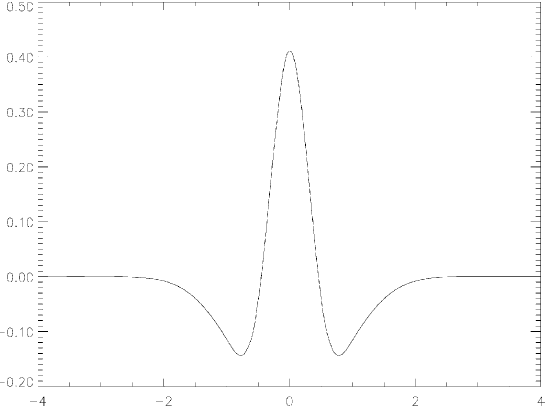
\includegraphics[width=0.3\linewidth]{./chapters/02.state/wavelet.png}
	\caption{The starlet wavelet in one dimension. Source: \cite{starck2015starlet}}
	\label{state:moresane:starlet}
\end{figure}

The starlet transform represents an image as a combination of starlet wavelets (shown in Figure \ref{state:moresane:starlet}) at different locations and scales. At the lowest scale, each starlet wavelet is a single pixel wide. At larger scales, each starlet wavelet spans over several pixels. It is an over-complete representation, because we can use several different combinations of starlet wavelets at different scales that lead to the same image.

Normally, we can only retrieve the image from the over-complete representation and not the other way around (because there are different combinations of starlets that lead to the same image). The starlet transform has a way to estimate its wavelet components from the dirty image. The MORESANE algorithm uses this property for reconstruction.

\begin{lstlisting}
dirtyImage = iFFT(Gridding(visibilities))
model = new Array[,]

do
	//estimate starlet components, dimensions: [x, y, scale]
	estimates = StarletTransform(dirtyImage, PSF)
	maxIndex = ArgMax(estimates)
	
	//find connected starlet components. Flood fill over the image(x, y) and over scales. Now we should have all starlets belonging to a single object (e.g. a hydrogen cloud or a single galaxy in the image)
	connectedStarlets = FloodFill(starlets, maxIndex)
	
	optimizedPixels = ConjugateGradients(connectedStarlets)
	
	//update dirty and model image
	model += optimizedPixels
	dirtyImage = dirtyImage - Convolve(optimizedPixels, PSF)
while
\end{lstlisting}

First, it uses the starlet transform on the dirty image, and search for the largest starlet component at a certain scale. The largest starlet component explains part of a single object emitting radio waves, like a hydrogen cloud or a galaxy. Next, we use the flood-fill algorithm to find all starlet components at all scales which describe this object.

The next step is the actual minimization step in the MORESANE algorithm: We use the conjugate gradient method and find the pixel patch, which explains the estimated starlet components. It is a convex optimization problem, similar to what we described in Section \ref{radio:cs}. But instead of searching for a whole image, we only minimize over a subset of the pixels:

\begin{equation}\label{state:moresane::cs:l2}
\underset{\bar{x}}{minimize} \: \left \| s_{estimate} - NS^\intercal(\bar{x} \star PSF) \right \|_2^2 \quad \bar{x} \geq 0
\end{equation}

Where $\bar{x}$ is the subset of the image we minimize, $S^\intercal$ is the starlet transform which transforms an image to starlet space, $N$ is a diagonal matrix which masks all non-zero starlets from the starlet transform, and $s_{estimate}$ are the connected starlet components we estimated. MORESANE reconstructs an image patch which most closely resembles the estimated starlet components.

Note that in this formulation, the reconstructed pixels of the object $\bar{x}$ are constrained to be non-negative. This is a common constraint in radio interferometric image reconstruction, as the radiation arriving at a pixel cannot be negative. However, we know from our tests that the WSCLEAN implementation of MORESANE does include negative pixels in the model image. The objective function \ref{state:moresane::cs:l2} shown here comes from the original MORESANE paper \eqref{state:moresane::cs:l2}, and  is not exactly used in every MORESANE implementation.





\newpage
\section{Coordinate descent deconvolution}\label{cd}
Coordinate descent methods are a family of algorithms. Various variants exist\cite{richtarik2016distributed, richtarik2016parallel}, but they share one common idea: Most of our problems become simple when we reduce the number of dimensions. Deconvolving a whole image is difficult. But deconvolving a single pixel is easy. As we will show in section \ref{cd:deriving}, we can derive a closed form solution\footnote{Deriving a formula which we can implement in a few lines of code.} for deconvolving a single pixel. We then iterate over all pixels, possibly several times, until we converge to a deconvolved image. 

This is the idea behind coordinate descent methods. By reducing the dimensions of the problem, we can often find an optimization algorithm where each iteration is "cheap" to compute. In these cases, coordinate descent methods produce competitive results\cite{nesterov2012efficiency, nesterov2013gradient}.

For a deconvolution algorithm in radio astronomy, we need three parts: An optimization algorithm, a regularization, and an optimization objective. We use coordinate Descent as the optimization algorithm, take Elastic Net as the regularization and use the following objective function:

\begin{equation}\label{cd:deconv}
\underset{x}{minimize} \: \frac{1}{2} \left \| I_{dirty} - x * PSF \right \|_2^2 + \lambda ElasticNet(x)
\end{equation}

As we have shown before, the objective function consists of two parts. The data term $\left \| I_{dirty} - x * PSF \right \|_2^2$ and the regularization term $ElasticNet(x)$. The data term forces the image to be as close to the measurements as possible which forces the image to be as close to the measurements as possible, the regularization term forces the image to be as consistent as possible with our prior knowledge. The parameter $\lambda$ is a weight that either forces more or less regularization. It is left to the user to define for each image. We will derive the coordinate descent algorithm that optimizes the objective \eqref{cd:deconv} in section \ref{cd:deriving}. First, let us explain what the elastic net regularization does.

\subsection{Elastic net regularization} \label{cd:reg}
\begin{figure}[h]
	\centering
	\begin{subfigure}[b]{0.3\linewidth}
		\includegraphics[width=\linewidth]{./chapters/03.distribution/L1.png}
		\caption{Effect of the pure L1 norm ($\lambda$ = 1.0) on a single point source.}
		\label{cd:elastic:L1}
	\end{subfigure}
	\begin{subfigure}[b]{0.3\linewidth}
		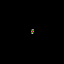
\includegraphics[width=\linewidth]{./chapters/03.distribution/L2.png}
		\caption{Effect of the pure L2 norm ($\lambda$ = 1.0) on a single point source.}
		\label{cd:elastic:L2}
	\end{subfigure}
	
	\caption{Effect of the L1 and L2 Norm separately.}
	\label{cd:elastic}
\end{figure}


This regularization is a mixture between the L1 and L2 regularization. The Figure \ref{cd:elastic} shows the effect of the L1 and L2 norm on a single star. The L1 regularization forces the image to contain few non-zero pixels as possible. It encodes our prior knowledge that the image will contain stars. The L2 regularization on the other hand "spreads" the single star across multiple pixels. This forces the image to represent extended emissions, like hydrogen cloud, with a large number of non-zero pixels (the L1 norm tends to break extended emissions apart, only using a handful of non-zero pixels). The L2 norm was already used in other image reconstruction algorithms in radio astronomy\cite{ferrari2014distributed}, with the downside that the resulting image will not be sparse.

Elastic net mixes these two norms together, becoming "sparsifying L2 norm". It retains the sparsifying property of the L1 norm, while also keeping extended emissions in the image. Formally, elastic net regularization is defined as the following:

\begin{equation}\label{cd:elastic:formula}
ElasticNet(x, \alpha) = \: \alpha \left \|x \right \|_1 + \frac{1-\alpha}{2}  \left \|x \right \|_2
\end{equation}

Elastic net has three properties which make it an interesting regularization for coordinate descent: It was shown to speed up convergence rates compared to the pure L1 or L2 norm\cite{friedman2010regularization}, is a separable function, and has a closed form solution. The first property was not further investigated in this work. The second property, separability, means that we can calculate the regularization for each pixel independently of each other, and we still arrive at the same result. Lastly, we can find a simple formula for each pixel that applies the elastic net regularization:

\begin{equation}\label{cd:elastic:closed}
ElasticNetClosedForm(x, \lambda ,\alpha) = \: \frac{max(x - \lambda * \alpha, 0)}{1+\lambda(1 - \alpha)}
\end{equation}

The closed form solution \eqref{cd:elastic:closed} of the elastic net regularization is also a mixture of the closed form solutions of the L1 and L2 norm. The closed form solution of the L1 norm is shrinkage: $max(x - \lambda, 0)$, we reduce the pixel value by $\lambda$ and clamp negative values. For the L2 norm, we divide the pixel value: $\frac{x}{1+\lambda}$.

%Proximal operator But the second property leads to an optimization algorithm 

Note that the shrink operation in this project always clamps negative pixels to zero. We constrain the image to only contain zero or positive pixel values. This has become a widely used constraint in radio interferometric image reconstruction and may lead to improved image quality\cite{mcewen2011compressed}.

Elastic net is the regularization we use throughout this work. It is separable (we can calculate it for each pixel independently) and has an easy to compute closed form solution.


\subsection{Deriving the basic coordinate descent deconvolution algorithm}\label{cd:deriving}
In this section we derive the basic coordinate descent deconvolution algorithm, which minimizes the objective \eqref{cd:deconv}. Coordinate descent methods have a tendency to need a more iterations to converge compared to other methods like gradient descent. However, when a single iteration is cheap to compute, they can be faster in practice\cite{shalev2011stochastic}. The elastic net regularization has an easy to compute closed form solution \eqref{cd:elastic:closed}, and a single iteration is cheap to compute.

We call the coordinate descent algorithm described here "basic". Other coordinate descent algorithms in the literature\cite{richtarik2016parallel,fercoq2015accelerated, richtarik2016distributed} can be seen as generalizations of the "basic" algorithm. The basic algorithm optimizes a single pixel at each iteration, while other algorithms can optimize one or several pixels. 
%We look at the basic coordinate descent algorithm first and use it as a baseline for comparing different coordinate descent algorithms.

In this section, we derive the basic coordinate descent algorithm that optimizes a single pixel in each iteration, and iterates over all pixels several times, with a specific strategy, until convergence. There are three types of iteration strategy we can choose:
\begin{enumerate}
	\item Random: where we choose a pixel to optimize uniformly at random.
	\item Greedy: where we first choose the pixel which minimizes our objective the most
	\item Cyclic: where we choose a subset of pixels and cycle through them until convergence. 
\end{enumerate}

The iteration strategy is not important for convergence. We can for example create a mixture of the different strategies and the algorithm would still converge to the optimum. However, the strategy we choose has an impact on how many iterations we need until convergence. For example: if the image consists of a single star in the center of the image, a greedy strategy would first optimize the pixel at the center, while a random strategy may waste the computing resources in checking every other pixel several times before finally landing on the center. In this implementation, we chose the greedy strategy. Each iteration takes the best possible step towards the optimum. We arrive at the following coordinate descent algorithm in pseudo code:


\begin{lstlisting}
dirty = IFFT(Gridding(visibilities))
residuals = dirty

x = new Array
objectiveValue = SUM(residuals * residuals) + P(x)
oldObjectiveValue = objectiveValue

do 
{
	oldObjectiveValue = objectiveValue

	//the core of the algorithm
	pixelLocation = GreedyStrategy(residuals)
	oldValue = x[pixelLocation]
	optimalValue = oldValue + Minimize(residuals, psf, pixelLocation)
	optimalValue = ApplyElasticNet(optimalValue, lambda, alpha)
	
	//housekeeping
	x[pixelLocation] = optimalValue
	residuals = residuals - PSF * (optimalValue - oldValue)
	objectiveValue = 0.5 * SUM(residuals * residuals) + lambda * ElasticNet(x, alpha)
} while (oldObjectiveValue - objectiveValue)  < epsilon
\end{lstlisting}

The core of the algorithm consists of the three functions: $GreedyStrategy()$, $Minimize()$ and $ApplyElasticNet()$. The function $GreedyStrategy()$ will be discussed in Section \ref{cd:efficient}. The function $ApplyElasticNet()$ was already described in equation \eqref{cd:elastic:closed}. The $Minimize()$ function is responsible for minimizing the data term of our objective \eqref{cd:deconv}. Because we only minimize a single pixel, we are dealing with a one dimensional minimization problem and can derive a closed form solution for it.

When we only have one pixel to minimize, the data term of our objective \eqref{cd:deconv} reduces itself to a parabola. We derive the standard parabola form in \eqref{cd:deriving:derivation}, where $\langle x, y\rangle$ is the inner product(element-wise multiplication followed by a sum over all elements):

\begin{equation} \label{cd:deriving:derivation}
\begin{split}
Minimize(pixel) & = \left \| I_{res} - PSF * pixel \right \|_2^2\\
Minimize(pixel) & = (I_{res} - PSF * pixel)^2\\
Minimize(pixel) & = \langle I_{res}, I_{res} \rangle - 2\langle I_{res},PSF\rangle * pixel + \langle PSF, PSF \rangle * pixel^2\\
Minimize(pixel) & = \langle PSF, PSF \rangle * pixel^2 - 2\langle I_{res},PSF\rangle * pixel + \langle I_{res}, I_{res} \rangle
\end{split}
\end{equation}

Now finding the optimal value for the pixel is the same as finding the optimal value of the parabola:

\begin{equation} \label{cd:deriving:minimizer}
\begin{split}
f(x) & = a*x^2 \\
 & + b*x \\
 & + c\\
 \\
x_{min} & = \frac{-b}{2a}
\end{split}
\quad \quad
\begin{split}
Minimize(pixel) & = \langle PSF, PSF \rangle * pixel^2 \\
 & - 2\langle I_{res},PSF\rangle * pixel \\
 &+ \langle I_{res}, I_{res} \rangle\\
 \\
pixel_{min} & = \frac{-(-2\langle I_{res},PSF\rangle)}{2\langle PSF, PSF \rangle}
\end{split}
\end{equation}

This means we can find the optimum value of a single pixel by following the formula in \eqref{cd:deriving:minimizer}. Note that the $PSF$ in formula \eqref{cd:deriving:derivation} and \eqref{cd:deriving:minimizer} is shifted to the pixel position we wish to optimize.

We derived the closed form solution \eqref{cd:deriving:minimizer} by looking at the data objective as a parabola. When we take another look at the closed form solution with Calculus in mind, we can see that the numerator $-2\langle I_{res},PSF\rangle)$ is actually the same as calculating the gradient for this pixel, and the denominator $\langle PSF, PSF \rangle$ is the Lipschitz constant. 

Intuitively, the Lipschitz constant describes how fast a function $f(x)$ changes with $x$. If $f(x)$ changes slowly, we can descend larger distances along the gradient without the fear for de-convergence. In short, it is a data-defined step size. Because our function $Minimize()$ is simply a parabola, the gradient together with the Lipschitz constant point to the optimum of our function.

Because the minimizer \eqref{cd:deriving:minimizer} of our coordinate descent algorithm calculates the gradient, one might ask what the differentiates the coordinate descent method from gradient descent. The main difference is that coordinate descent uses the gradient of a single pixel (or subset of pixels in other versions), in each iteration, while gradient descent generally uses the gradients of all pixels in each iteration. Conceptually, coordinate descent does is not bound to use the gradient. We could also minimize the pixel with a line-search algorithm, trying different values for the pixel, and it is still a coordinate descent method.

This is how the basic coordinate descent deconvolution algorithm works. But as it is described here, one iteration is too expensive to be practical. The $Minimize()$ function calculates both the gradient and the Lipschitz constant in each iteration and the residual update in line 20 requires a convolution. We can drastically improve the runtime costs by caching intermediate results, and using approximations.

\subsection{Efficient implementation of basic coordinate descent deconvolution}\label{cd:efficient}
In Section \ref{cd:deriving}, we derived the basic coordinate descent deconvolution algorithm. There are several "tricks" to speed up each iteration. We can cache intermediate results, and exploit the convolution to efficiently calculate the inner products of the basic algorithm We discuss:

\begin{enumerate}
	\item Edge handling of the convolution
	\item Pre-calculation of the Lipschitz constants
	\item Efficient greedy strategy
 	\item Pre-calculation of gradients
	\item Efficient update of gradients
\end{enumerate}

Gradient calculation is the most time consuming step. We can exploit the convolution to efficiently pre-calculate, update and approximate the gradients for each pixel. This will be discussed in detail in this Section. To our knowledge, we are the first to explore ways to approximate the gradient in radio interferometric image reconstruction, and their effect on parallel and distributed deconvolution. As we will se in the later sections, approximating the gradients can help us to distribute the deconvolution. 

Visual aid:
\begin{figure}[h]
	\centering
	\begin{subfigure}[b]{0.3\linewidth}
		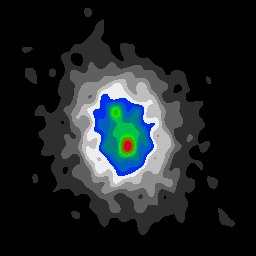
\includegraphics[width=\linewidth]{./chapters/03.distribution/simulated/dirty.png}
		\caption{Dirty Image.}
		\label{cd:efficient:aid:dirty}
	\end{subfigure}
	\begin{subfigure}[b]{0.3\linewidth}
		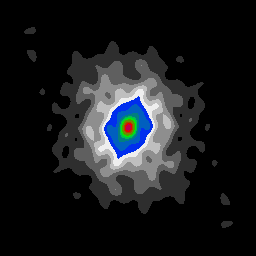
\includegraphics[width=\linewidth]{./chapters/03.distribution/simulated/psf.png}
		\caption{Point Spread Function.}
		\label{cd:efficient:aid:psf}
	\end{subfigure}
	\begin{subfigure}[b]{0.3\linewidth}
		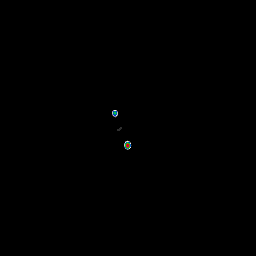
\includegraphics[width=\linewidth]{./chapters/03.distribution/simulated/elastic.png}
		\caption{ElasticNet deconvolution}
		\label{cd:efficient:aid:elastic}
	\end{subfigure}
	
	\caption{Example problem with two point sources.}
	\label{cd:efficient:aid:figure}
\end{figure}

First, we dive into the implementation of the convolution operator and the pre-calculation of the Lipschitz constants, and then we discuss the gradient calculation in detail.

\subsubsection{Edge handling of the convolution}
As the reader is probably aware, there are several ways to define the convolution in image processing, depending on how we handle the edges on the image. Two possibilities are relevant for radio interferometric image reconstruction: Circular and zero padded.

\begin{figure}[h]
	\centering
	\begin{subfigure}[b]{0.3\linewidth}
		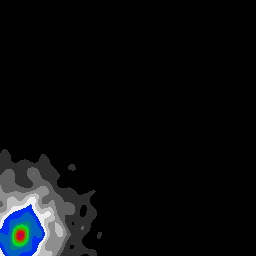
\includegraphics[width=\linewidth]{./chapters/03.distribution/simulated/padded.png}
		\caption{Zero padded convolution.}
		\label{cd:efficient:convolution:padded}
	\end{subfigure}
	\begin{subfigure}[b]{0.3\linewidth}
		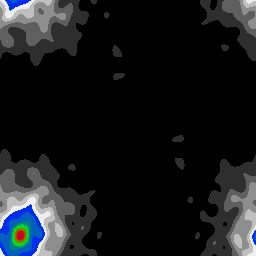
\includegraphics[width=\linewidth]{./chapters/03.distribution/simulated/circular.png}
		\caption{Circular convolution.}
		\label{cd:efficient:convolution:circular}
	\end{subfigure}
	\caption{Comparison of the two convolution schemes.}
	\label{cd:efficient:convolution:figure}
\end{figure}

Circular convolution assumes the image "wraps" around itself. If we travel over the right edge of the image, we arrive at the left edge. The convolution in Fourier space is circular. Remember: A convonlution in image space is a multiplication in Fourier space, and vice versa. When we convolve the reconstructed image $x$ with the $PSF$ using circular convolution, then non-zero pixels at the right edge of the image "shine" over to the left edge. This is physically impossible.

Zero padding assumes that after the edge, the image is zero. Non-zero pixels at the right edges of the image do not influence the left edge after convolution. This is the physically plausible solution. However, the zero padded convolution is more expensive to calculate. We either have to calculate the convolution in image space, which is too expensive for large kernels, or apply the FFT on a zero-padded image. Either way, it is more expensive than the circular convolution.

In designing a deconvolution algorithm, we have the choice between the circular and the zero-padded convolution scheme. Circular convolution is more efficient to calculate, while zero-padded convolution is closer to the reality. Both choices are possible. The PyMORESANE reconstruction algorithm \cite{kenyon2019pymoresane} leaves this choice to the user. We decided on using the zero-padded convolution. This choice influences other parts of the coordinate descent deconvolution algorithm, like how we can efficiently calculate the Lipschitz constants.

\subsubsection{Pre-calculation of the Lipschitz constants}
Lipschitz constants are $\langle PSF, PSF \rangle$. We simply multiply the $PSF$ with itself and sum up the values. However, we are using the zero-padded convolution. This means the $PSF$ for pixels at the edges is not only shifted, but also cropped. In other words, every pixel has a different Lipschitz constant depending on how much the $PSF$ gets cropped by the image edges.

Note that it is not an issue for convergence: The Lipschitz constant describes the largest step we can take without overshooting the target. We can always make smaller steps, but may pay it with more iterations. The Lipschitz constant of the edge pixels is always lower than the center. The coordinate descent algorithm does converge, but needs more iterations for pixels at the edges of the image. Luckily, there is a way to re-use intermediate results, and efficiently calculate the Lipschitz constant for each pixel in the image.

The first observation is that the image edges always create a rectangular crop of the $PSF$. To calculate the Lipschitz constant, we square and sum up all the values that lie inside the rectangle. This can be exploited with a scan algorithm: We store the $PSF$ as a running sum of squares. 

\begin{lstlisting}
var scan = new double[,];
for (i in (0, PSF.Length(0))
{
	for (j in (0, PSF.Length(1))
	{
		var iBefore = scan[i - 1, j];
		var jBefore = scan[i, j - 1];
		var ijBefore = scan[i - 1, j - 1];
		var current = PSF[i, j] * PSF[i, j];
		scan[i, j] = current + iBefore + jBefore - ijBefore;
	}
}
\end{lstlisting}

$scan[0, 13]$ contains the sum of the squared $PSF$ values from index $(0,0)$ up to and including index $(0, 13)$. The last element, $scan[PSF.Length(0) - 1, PSF.Length(1) -1]$ contains the sum of squares over the whole $PSF$. In short, we have stored the sum of all possible rectangles starting from index $(0,0)$. If a part of the $PSF$ is cropped, we can look up $scan$ and find out by how much it affects the total sum.

Up to 4 

%Numerical issues with float precision.

\subsubsection{Efficient Greedy strategy}

Calculate what each update would lead to what objective.
Expensive to calculate.

However, we can use another strategy, we use the biggest change in pixel value.
A lot cheaper to compute
Biggest change in pixel value is in toy examples the same as the best pixel. 

Not sure if this is always true.


\subsubsection{Pre-calculation of gradients}
In each iteration, we need to know the gradient for all pixels. We need to calculate the inner product $\langle I_{res},PSF\rangle$ for each pixel. Typically, the $PSF$ and the image have the same number of pixels, which leads to a quadratic number of operations to calculate all gradients.

Luckily, we can use the Fourier transform to speed up the calculation. Notice that the inner product $\langle I_{res},PSF\rangle$ is equivalent to calculating the correlation of the residuals with the $PSF$ ($)I_{res} \star PSF$). The convolution and correlation operators are related: The convolution is equal to a correlation with a flipped kernel. Since a convolution in image space is a multiplication in Fourier space, we can calculate the $PSF$ correlation efficiently in Fourier space.

\begin{figure}[h]
	\centering
	\begin{subfigure}[b]{0.3\linewidth}
		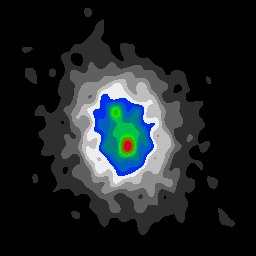
\includegraphics[width=\linewidth]{./chapters/03.distribution/simulated/dirty.png}
		\caption{Dirty Image.}
		\label{cd:efficient:gradients:dirty}
	\end{subfigure}
	\begin{subfigure}[b]{0.3\linewidth}
		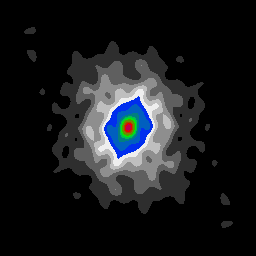
\includegraphics[width=\linewidth]{./chapters/03.distribution/simulated/psf.png}
		\caption{Point Spread Function.}
		\label{cd:efficient:gradients:psf}
	\end{subfigure}
	\begin{subfigure}[b]{0.3\linewidth}
		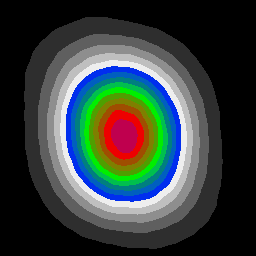
\includegraphics[width=\linewidth]{./chapters/03.distribution/simulated/gradients.png}
		\caption{Gradient for each pixel.}
		\label{cd:efficient:gradients:gradients}
	\end{subfigure}
	
	\caption{Example of the gradient calculation.}
	\label{cd:efficient:gradients:figure}
\end{figure}

The Figure \ref{cd:efficient:gradients:figure} shows the process for the first step of the coordinate descent deconvolution. We start with the dirty image. We calculate the correlation of the $PSF$ with the dirty image and arrive at the map of gradients. Figure \ref{cd:efficient:gradients:gradients} shows the gradient for each pixel.

\subsubsection{Efficient update of gradients}
The naive coordinate descent implementation minimizes a single pixel, and updates the residuals by subtracting the $PSF$ at the correct location (The first line of \eqref{cd:efficient:update:naive}). It then calculates the new gradient for each pixel(Second line of \eqref{cd:efficient:update:naive}) in each iteration. This is not necessary. We only need to calculate the correlation in the first iteration. All later iterations update the map gradients directly without the Fourier transform.

\begin{equation}\label{cd:efficient:update:naive}
\begin{split}
residuals &= residuals - PSF * (optimalValue - oldValue) \\
gradients &= residuals \star PSF
\end{split}
\end{equation}

The trick is to combine both lines of the naive update \eqref{cd:efficient:update:naive}. We correlate each term of the first line with the $PSF$, and we arrive at the update rule \eqref{cd:efficient:update:new}.

\begin{equation}\label{cd:efficient:update:new}
gradients = gradients - (PSF \star PSF) * (optimalValue - oldValue)
\end{equation}

The noteworthy part of \eqref{cd:efficient:update:new} is that we update the gradients directly, but instead of using the $PSF$, we take the product of $(PSF \star PSF)$, of the $PSF$ correlated with itself. Also note that we do not need to keep the residuals in memory. All we need is the map of gradients. 

\begin{figure}[!h]
	\centering
	\begin{subfigure}[b]{0.3\linewidth}
		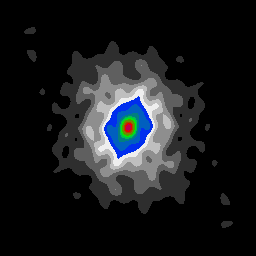
\includegraphics[width=\linewidth]{./chapters/03.distribution/simulated/psf.png}
		\caption{Point Spread Function.}
		\label{cd:efficient:update:dirty}
	\end{subfigure}
	\begin{subfigure}[b]{0.3\linewidth}
		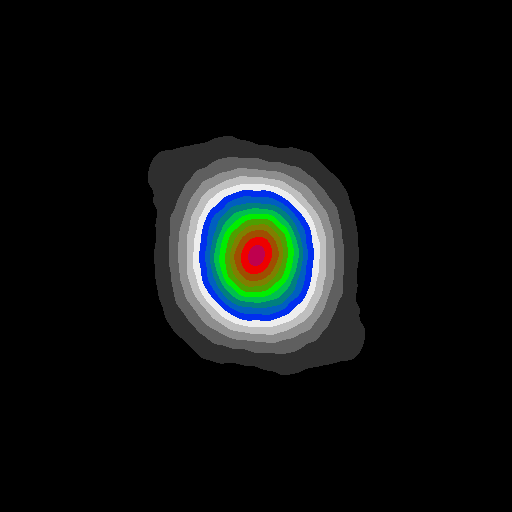
\includegraphics[width=\linewidth]{./chapters/03.distribution/simulated/psf2.png}
		\caption{Gradient update: $(PSF \star PSF)$.}
		\label{cd:efficient:update:psf}
	\end{subfigure}
	\caption{Example problem with two point sources.}
	\label{cd:efficient:update:figure}
\end{figure}

Calculate the PSF correlation with itself. Calculate the PSF correlation once, and use it to update the gradient map directly.

Edges again. We have the problem that, when the PSF is cutoff by the edges of the image, we would need to calculate $(PSF \star PSF)$ again. This is too expensive. Does not change dramatically, unless the pixel we optimize is at the full edge.


\subsection{Similarities to the CLEAN algorithm}

Comparison to CLEAN. Similar algorithm, but we descend in the actual gradient direction.

\subsection{Pseudo-code of the basic, optimized algorithm}

putting it all together




GPU implementation




\subsection{Distributed Deconvolution}
How do we distribute the major cycle. We need to distribute every step, Gridding, FFT and Deconvolution.

Gridding, Large number of input data. This needs to be distributed
We use the Image domain gridding introduces in sectionand use it as the basis for the distributed gridding.

The FFT is generally not worth distributing, if we can keep all the data in memory. When the gridding is done, in our setup, the grid is small enough to keep in memory. (cite distributed fftw)

Deconvolution is also worth distributing. CLEAN depending on the observation is the second most time consuming step. But gridding tends to be easier to distribute, so in some observations it is the most time consuming step.
Split the image into patches and deconvolve each patch.
Sadly not possible, we need communication. how we communicate is important.

We use a distributed Gridding and a distributed deconvolution. Which leads us to the following architecture.

\begin{figure}[h]
	\centering
	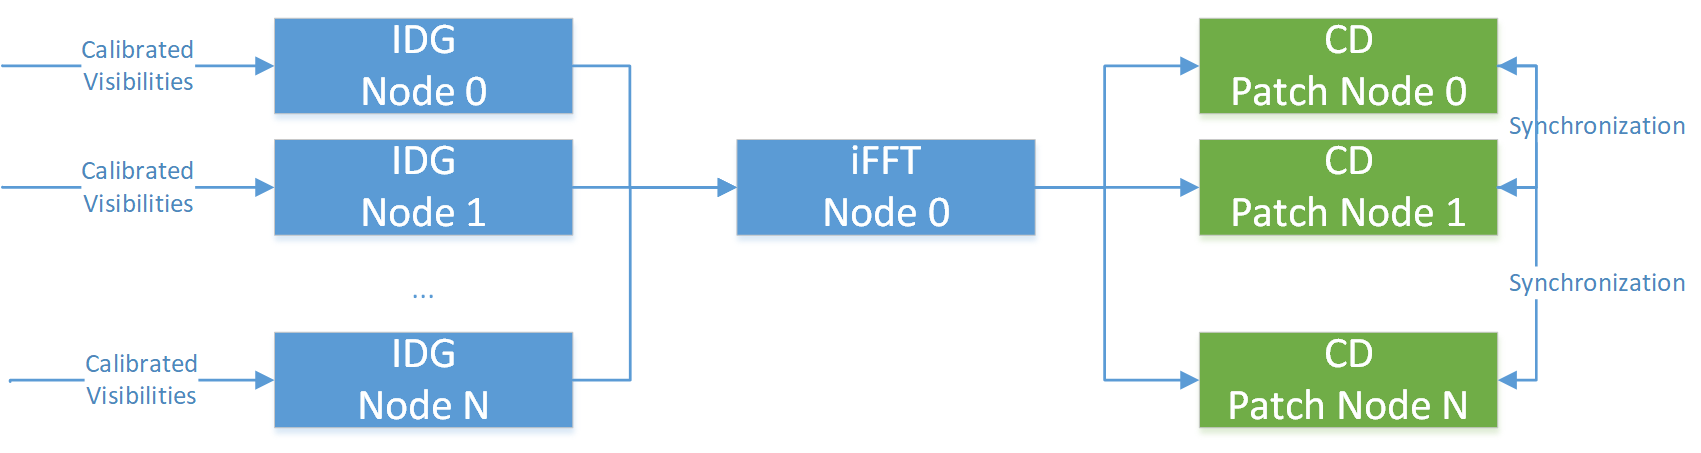
\includegraphics[width=0.80\linewidth]{./chapters/03.distribution/distributed_architecture.png}
	\caption{Distributed architecture for half a major cycle}
	\label{dist:architecture:fig}
\end{figure}

Where each node is one computer, i.e. has its own, possibly multiple cpus and its shared memory.
Split the input visibilities onto nodes. 
Do the gridding locally on each node
Communicate the grid
inverse FFT on one node.
Communicate the patches of the image.
Deconvolve each patch and communicate

\newpage
\section{Serial coordinate descent deconvolution}\label{cd}
In this section, we introduce the serial coordinate descent algorithm, which can replace CLEAN in the Major/Minor cycle architecture. We call this algorithm 'serial', because it minimizes exactly a single pixel in each iteration. Later in In Section \ref{pcdm} we introduce the parallel coordinate descent algorithm, which optimizes multiple pixels in a single iteration (multiple pixels in parallel).

In this project, the serial and parallel coordinate descent algorithm minimize the following convex objective function:

\begin{equation}\label{cd:deconv}
\underset{x}{minimize} \: \frac{1}{2} \left \| I_{dirty} - x * PSF \right \|_2^2 + \lambda ElasticNet(x)
\end{equation}

We want to find the minimum deconvolved image $x$, which is as close to the dirty image (remember the dirty image results from the visibilities, which get gridded and transformed to image space), but also has the smallest regularization penalty. The parameter $\lambda$ is a weight that either forces more or less regularization. It is either left to the user to define for each image, or can be estimated from the data \cite{miller1970least}. In this project, we leave $\lambda$ for the user to define. The objective function \eqref{cd:deconv} is convex, and we can use convex optimization methods to find a reconstructed image $x$. 

First, dive deeper into the elastic net regularization, and then continue with introducing the serial coordinate descent algorithm in Section \ref{cd:serial}. Although we call the algorithm 'serial', its implementation can use multiple processors in certain steps of the algorithm: For example updating a rectangle of pixels in the residual image can be trivially performed with multiple processors. We also created a GPU-accelerated and a distributed implementation of the serial coordinate descent algorithm. They can be found in the attachments, since both GPU-accelerated and distributed implementations were slower than the final CPU implementation of the parallel coordinate descent algorithm.

\subsection{Elastic net regularization} \label{cd:reg}
This regularization is a mixture between the L1 and L2 norm. The L1 norm is the absolute value of all pixels ($\left \| x \right \| = \sum_i \sum_j \left \| x_{ij} \right \|$), and the L2 norm is the squared sum of all pixels ($\left \| x \right \|_2 = \sum_i \sum_j \left \| x_{ij} \right \|^2$). The Figure \ref{cd:elastic} shows the effect of the L1 and L2 norm on a single star. The L1 norm forces the image to contain few non-zero pixels as possible. It encodes our prior knowledge that the image will contain stars. The L2 regularization on the other hand "spreads" the single star across multiple pixels, which helps reconstructing extended emissions.

\begin{figure}[h]
	\centering
	\begin{subfigure}[b]{0.4\linewidth}
		\includegraphics[width=\linewidth]{./chapters/03.CD/L1.png}
		\caption{Effect of the pure L1 norm ($\lambda$ = 1.0) on a single point source.}
		\label{cd:elastic:L1}
	\end{subfigure}
	\begin{subfigure}[b]{0.4\linewidth}
		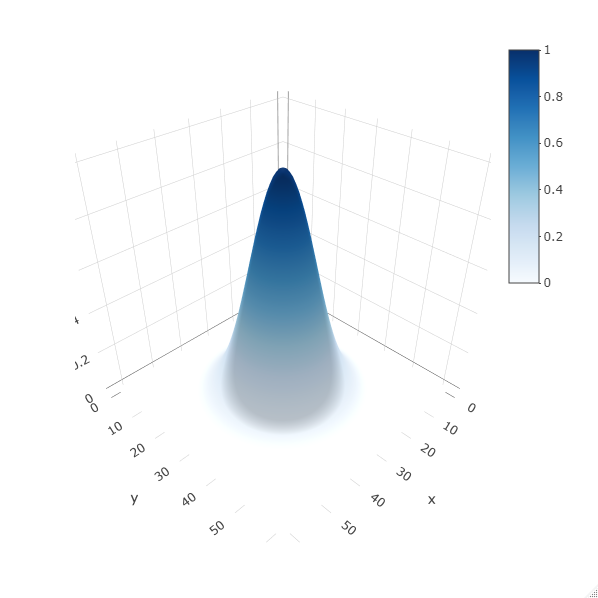
\includegraphics[width=\linewidth]{./chapters/03.CD/L2.png}
		\caption{Effect of the pure L2 norm ($\lambda$ = 1.0) on a single point source.}
		\label{cd:elastic:L2}
	\end{subfigure}
	
	\caption{Effect of the L1 and L2 Norm separately.}
	\label{cd:elastic}
\end{figure}

The L1 regularization alone models an image that consists of points sources. For extended emissions like hydrogen clouds, the L1 norm alone may force the algorithm to approximate the cloud with point sources. The L1 norm alone is not a good model for radio interferometric images that contain extended emissions. The L2 norm alone was already used in other image reconstruction algorithms in radio astronomy\cite{ferrari2014distributed}, with the downside that the resulting image will not be sparse. I.e. all pixels in the reconstruction will be non-zero, even though some of them only contain noise. 

Elastic net mixes the L1 and L2 norm together, becoming "sparsifying L2 norm". It retains the sparsifying property of the L1 norm, while also keeping extended emissions in the image. Formally, elastic net regularization is defined as the following regularization function:

\begin{equation}\label{cd:elastic:formula}
ElasticNet(x, \alpha) = \: \alpha \left \|x \right \|_1 + \frac{1-\alpha}{2}  \left \|x \right \|_2
\end{equation}

The parameter $\alpha$ is between 0 and 1, and mixes the two norms together. A value of 1 leads to L1 regularization only, and a value of 0 leads to L2 only. The elastic net regularization has two properties, which are relevant later for the serial coordinate descent algorithm: It is separable, and has a proximal operator.

Separability means that we can calculate the elastic net regularization penalty independently for each pixel. We arrive at the same result if we evaluate \eqref{cd:elastic:formula} for each pixel and sum up the results, or if we evaluate \eqref{cd:elastic:formula} for the whole image. This is an important property when one tries to minimize the objective function \eqref{cd:deconv} used in this project. We can minimize a single pixel at a time, and do not need to account for the whole neighborhood.

The proximal operator of elastic net allows us to minimize the regularization penalty. Notice that the elastic net regularization \eqref{cd:elastic:formula} is not differentiable (the L1 norm is not continuous). We cannot calculate a gradient. However, it has a proximal operator defined:

\begin{equation}\label{cd:elastic:proximal}
ElasticNetProximal(x, \lambda ,\alpha) = \: \frac{max(x - \lambda \alpha, 0)}{1+\lambda(1 - \alpha)}
\end{equation}

The proximal operator allows us to minimize the deconvolution problem with an elastic net regularization. We can calculate the gradient of the data term of \eqref{cd:deconv}, which is differentiable. Then, we apply the proximal operator on the gradients. Descending these modified gradients minimizes the objective function \eqref{cd:deconv}. The proximal operator of elastic net can be applied on the gradient of each pixel independently. Neighboring pixels do not influence the regularization.

A side note on the proximal operator used in this project \eqref{cd:elastic:proximal}: The numerator always clamps negative pixels to zero. This is a conscious design decision. In radio astronomy, it is usual to constrain the reconstruction to be non-negative (because we cannot receive negative radio emissions from any direction). It is widely used in radio astronomy image reconstruction and may lead to improved reconstruction quality \cite{mcewen2011compressed}.


\subsection{Serial coordinate descent algorithm}\label{cd:serial}
Our serial coordinate descent deconvolution algorithm minimizes the deconvolution objective \eqref{cd:deconv} for a single pixel at each iteration. Each iteration consists of two steps. Step 1: Find the best pixel to optimize. Step 2: Calculate the gradient for this pixel, apply the elastic net proximal operator, and take the descent s take a descent step for the single pixel. The algorithm iterates over all pixel multiple times to converge to a reconstructed image.

We demonstrate the serial deconvolution algorithm with the help of a simulated MeerKAT reconstruction problem of two point sources. Figure \ref{cd:serial:aid:dirty} shows the dirty image of two point sources, and Figure \ref{cd:serial:aid:psf} the $PSF$. The deconvolved image with elastic net regularization is shown in Figure \ref{cd:serial:aid:elastic}. I.e. Figure \ref{cd:serial:aid:elastic} is the optimum $x$ of the objective function \eqref{cd:deconv}.

\begin{figure}[h]
	\centering
	\begin{subfigure}[b]{0.3\linewidth}
		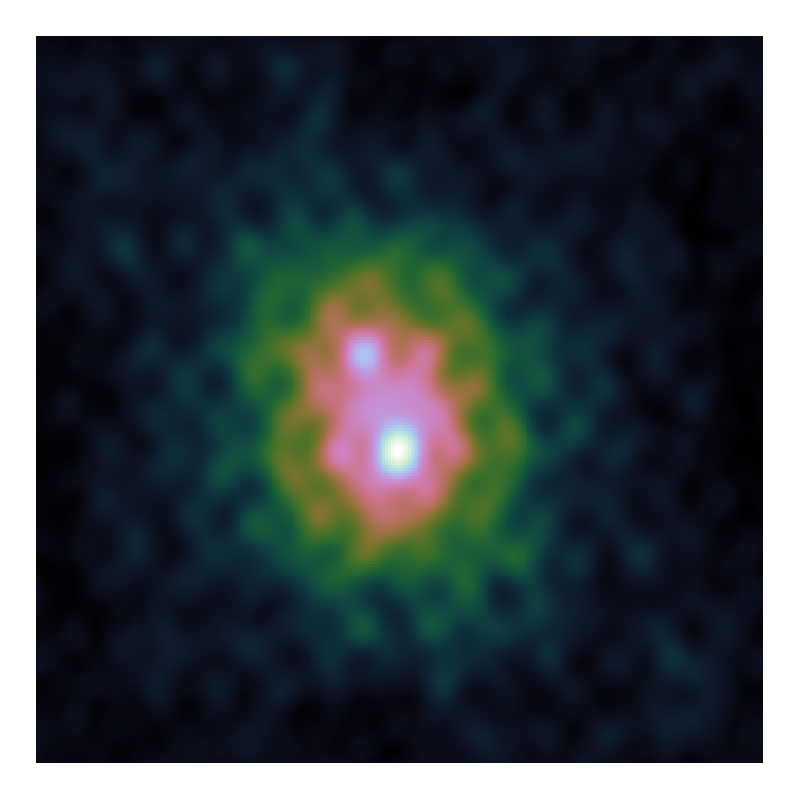
\includegraphics[width=\linewidth, clip, trim= 0.25in 0.25in 0.25in 0.25in]{./chapters/03.cd/simulated/dirty.png}
		\caption{Dirty Image.}
		\label{cd:serial:aid:dirty}
	\end{subfigure}
	\begin{subfigure}[b]{0.3\linewidth}
		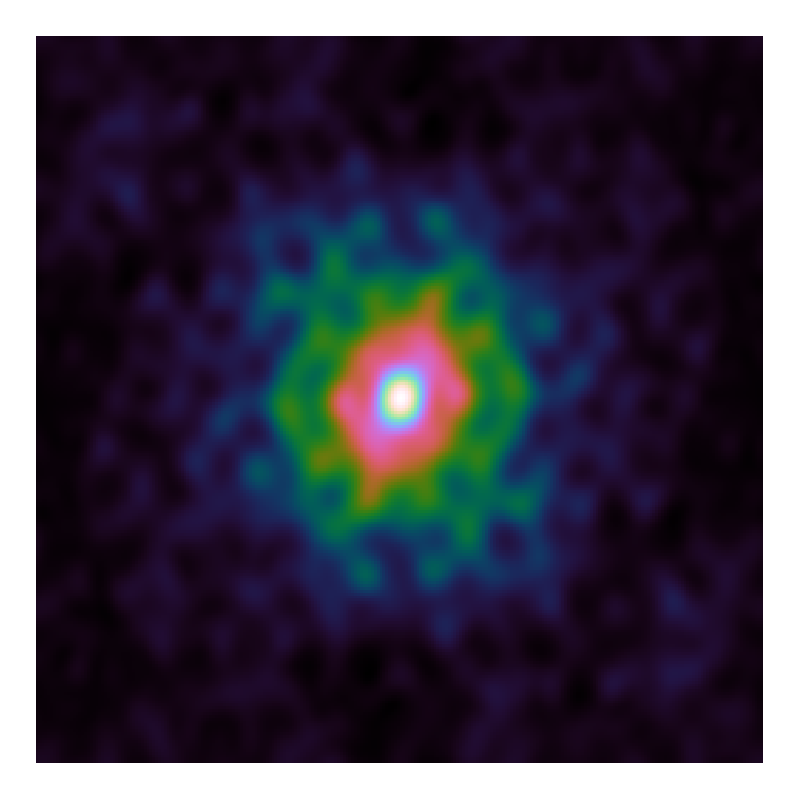
\includegraphics[width=\linewidth, clip, trim= 0.25in 0.25in 0.25in 0.25in]{./chapters/03.cd/simulated/psf.png}
		\caption{Point Spread Function.}
		\label{cd:serial:aid:psf}
	\end{subfigure}
	\begin{subfigure}[b]{0.3\linewidth}
		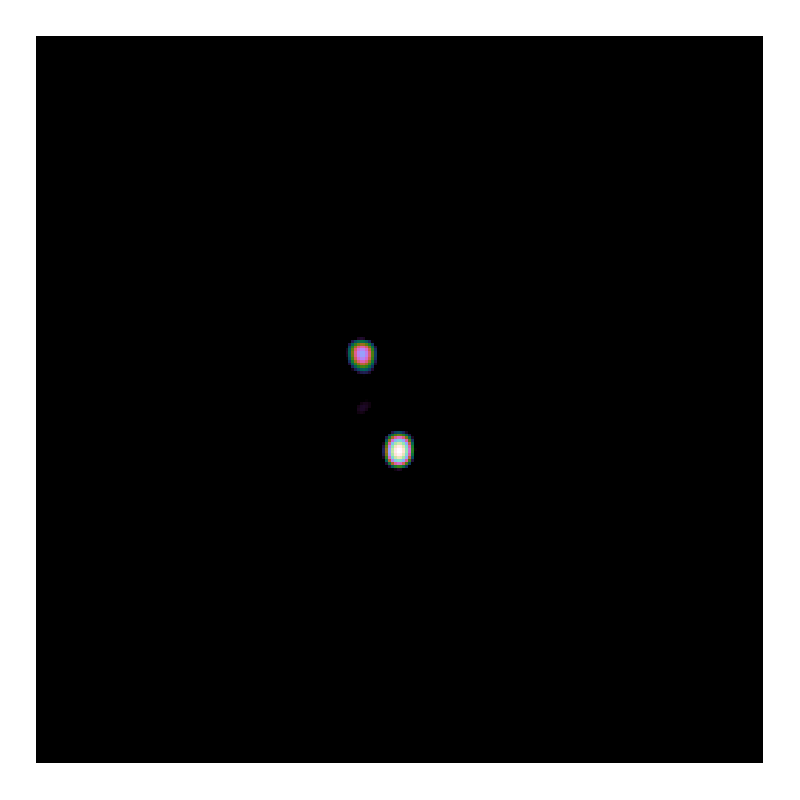
\includegraphics[width=\linewidth, clip, trim= 0.25in 0.25in 0.25in 0.25in]{./chapters/03.cd/simulated/elasticNet.png}
		\caption{Elastic net reconstruction}
		\label{cd:serial:aid:elastic}
	\end{subfigure}

	\caption{Example problem with two point sources.}
	\label{cd:serial:aid:figure}
\end{figure}

\subsubsection{Step 1: Choosing single a pixel}
For coordinate descent methods, there are several strategies to choose a single coordinate (pixel). Our serial coordinate descent algorithm uses a greedy strategy. In the first step, we iterate over all pixels and calculate its gradient. We select the pixel with which has the largest gradient magnitude. In each iteration, the greedy strategy chooses the pixel, which results in the largest decrease of our objective function \eqref{cd:deconv}. There are two other strategies that are often used in coordinate descent methods: Random and Cyclic.
%with the maximum possible difference in this iteration

A random strategy chooses, as the name implies, a pixel at random. Usually, the pixels are chosen from a uniform distribution. The random strategy leads to cheaper iteration compared to the greedy strategy, because we do not check the gradient of each pixel.

A cyclic strategy iterates over a subset of pixels until the subset converges. It then chooses another subset. Each iteration of the cyclic strategy is also cheaper than the greedy strategy. 

For our image deconvolution problem, we choose the greedy strategy. Even though it is more expensive, it tends to be faster to converge on the deconvolution problem in radio astronomy. Our reconstructed image is sparse, meaning most pixels in the image will be zero. The greedy strategy tends to choose pixels which will be non-zero in the final reconstructed image. While the random or cyclic strategy will set pixels to a non-zero value, which will eventually become zero in the final image. For the deconvolution problem, removing pixels from an intermediate solution seems to slow down the time to converge. We will discuss the different selection strategies in detail for the parallel coordinate descent methods.


\subsubsection{Step 2: Optimizing a single pixel}
At this point, the greedy strategy has selected a pixel at a specific location to minimize. The serial coordinate descent algorithm minimizes a single pixel at each iteration, and our deconvolution objective \eqref{cd:deconv} is reduced from a large number of dimensions (pixels), to a one dimensional problem\footnote{The reason why this reduces nicely to one dimension is the elastic net regularization is separable. I.e. the regularization can be calculated independently of the surrounding pixels.}:  

\begin{equation}\label{cd:serial:step2:onedim}
\underset{x}{minimize} \: \frac{1}{2} \left \| I_{dirty} - x_{location} * PSF \right \|_2^2 + \lambda ElasticNet(x_{location})
\end{equation}

Optimizing the one dimensional problem \eqref{cd:serial:step2:onedim} is a lot simpler. In essence, we calculate the gradient for the pixel at the selected location, and apply the proximal operator of elastic net. First, let us look at how the gradient is calculated and ignore the regularization. The gradient arises from the data term of the one dimensional objective \eqref{cd:serial:step2:onedim} ($\left \| I_{dirty} - x_{location} * PSF \right \|_2^2$). After simplifying the partial derivative, we arrive at the calculation:

\begin{equation}\label{cd:serial:step2:gradient}
\begin{split}
residuals &= I_{dirty} - x * PSF \\
gradient_{location} &= \langle residuals, PSF_{location} \rangle \\
Lipschitz_{location} &= \langle PSF_{location}, PSF_{location} \rangle \\
pixel_{opt} &= \frac{gradient_{location}}{Lipschitz_{location}}
\end{split}
\end{equation}

First, we calculate the residuals by convolving the current solution $x$ with the $PSF$. Then, the gradient for the selected pixel location is the inner product(element-wise multiplication followed by a sum over all elements) of the residuals and the $PSF$, shifted at the current location. The next step is to calculate the Lipschitz constant at the current location. Finally, we arrive at the optimal pixel value by dividing the gradient with the Lipschitz constant (The optimal deconvolved pixel value, ignoring the regularization).

The Lipschitz constant can be thought of as the step size. It defines how far we can descend towards the direction of the gradient. The Lipschitz constant describes how fast a function $f(x)$ changes with $x$. If $f(x)$ changes slowly, we can descend larger distances along the gradient without the fear for divergence. The Lipschitz constant can be looked at as a data-defined step size.

An interesting point is that the update rule $pixel_{opt} = \frac{gradient_{location}}{Lipschitz_{location}}$ finds the optimal pixel value, if the pixel is independent. Remember that our objective function is convex. The data term of our one dimensional objective \eqref{cd:serial:step2:onedim} actually forms a parabola, with the parameters: $x^2 \langle PSF, PSF \rangle - 2x \langle resdiuals, PSF_{location}\rangle + c$. Calculating the optimum of the parabola $\frac{-b}{2a}$, is identical to calculating the gradient update \eqref{cd:serial:step2:gradient}. Note that $b = -2 gradient_{location}$ and $a = Lipschitz_{location}$, and both the minimum of the parabola $\frac{-b}{2a}$ and the update rule based on partial derivatives \eqref{cd:serial:step2:gradient} are identical.

This means if our reconstruction problem has point sources which are far away, such that their $PSF$s do not overlap, then the update rule finds the optimal value for each point source with one iteration. But when the $PSF$s overlap as in our example problem, shown in Figure \ref{cd:serial:aid:figure}, then we need several iterations to sort out the correlated pixels. The serial coordinate descent algorithm needs to iterate over the same pixel several times until it converges.

\textbf{Including the elastic net regularization}\\
So far, we ignored the regularization. We can calculate the optimal pixel value without elastic net regularization. The last step is to combine the proximal operator of the elastic net regularization \eqref{cd:elastic:proximal} with the gradient calculation, and we arrive at the following update step:

\begin{equation} \label{cd:serial:step2:update}
pixel_{opt} = \frac{max(gradient_{location} - \lambda\alpha, 0)}{Lipschitz_{location} + (1 - \alpha)\lambda}
\end{equation}

This update rule now finds the optimal pixel value with elastic net regularization. If the $PSF$s do not overlap, we still only need one iteration per source.

Note that our algorithm calculates the gradient for a single pixel in each iteration. This may raise the question: What exactly is the difference between gradient- and coordinate descent? The difference is that gradient descent optimizes all pixels in each iteration, while coordinate descent optimizes (generally) a single pixel at a time\footnote{There are block coordinate descent methods that optimize a block of coordinates at each iteration. They are also discussed together with parallel coordinate descent methods in Section \ref{pcdm}}. Also, Coordinate descent methods are not bound to use the gradient. It could use a line search approach, where we try different values and decide on the one leading to the lowest objective value.

Optimizing a single pixel at a time can be an advantage for the deconvolution problem. There is a trade-off between descending a single pixel at a time, or a group of pixels: A gradient based algorithm can change a large value of a single pixel, or a smaller value for a group of pixels without the danger of diverging. The more pixels are changed in every iteration, the smaller the change can be for each pixel. In the deconvolution problem, large parts of the reconstructed image will be zero. We want the optimization algorithm to focus its changes on pixels, which are non-zero in the final reconstruction.

Now we put together our serial coordinate descent algorithm, and show where the bottleneck lies. In each iteration, the serial coordinate descent algorithm selects the pixel with the maximum gradient magnitude, and optimizes the selected pixel with the update rule \eqref{cd:serial:step2:update}.

\begin{lstlisting}
dirty = IFFT(GridVisibilities(visibilities))
residuals = dirty

x = new Array
objectiveValue = 0.5* Sum(residuals * residuals) + ElasticNet(x)

diff = 0
do 
	oldObjectiveValue = objectiveValue
	
	//Step 1: Search pixel
	pixelLocation = GreedyStrategy(residuals, PSF)
	oldValue = x[pixelLocation]
	shiftedPSF = Shift(PSF, pixelLocation)
	
	//Step 2: Optimize pixel
	gradient = Sum(residuals * shiftedPSF)
	lipschitz = Sum(shiftedPSF * shiftedPSF)
	tmp = gradient + oldValue * lipschitz 
	optimalValue = Max(tmp - lambda*alpha) / (lipschitz + (1 - alpha)*lambda)
	x[pixelLocation] = optimalValue

	//housekeeping
	diff = newValue - oldValue
	residuals = residuals - shiftedPSF * (optimalValue - oldValue)
while epsilon < Abs(diff) 
\end{lstlisting}

The actual update step is cheap to compute. We are only dealing with 4 one dimensional variables. The expensive calculations are the inner products: The gradient calculation, the Lipschitz constant and the objective value. The residuals and $PSF$ generally contain millions of pixels. Calculating the inner product of those becomes expensive. 

Also note that the greedy strategy needs to calculate the gradient for each pixel. As it is, the greedy strategy has a quadratic runtime complexity. 

\subsection{Efficient implementation}\label{cd:efficient}
Because coordinate descent methods only optimize a single pixel at a time, they generally need a large number of iterations to converge compared to other methods. But when each iteration is cheap to compute, coordinate descent methods can converge to a result in less time than competing methods\cite{nesterov2012efficiency, nesterov2013gradient}. We now discuss the efficient implementation.

The bottleneck of the serial coordinate descent algorithm are all the inner products that need to be calculated in each iteration. In each iteration, we need to know the gradient for every pixel, and the Lipschitz constant of the current pixel. Luckily, we can cache a map of gradients, where we save the gradient for every pixel and skip all of the inner products associated with the gradient. The Lipschitz constants are, as the name implies, constant for the whole deconvolution. They can be pre-calculated and cached for each pixel. The efficient calculation of Lipschitz constants can be found in the Attachments. We can greatly reduce the runtime cost for each iteration.


\subsubsection{Edge handling of the convolution}
As the reader is probably aware, there are several ways to define the convolution in image processing, depending on how we handle the edges on the image. Two possibilities are relevant for radio interferometric image reconstruction: Circular and zero padded.

\begin{figure}[h]
	\centering
	\begin{subfigure}[b]{0.3\linewidth}
		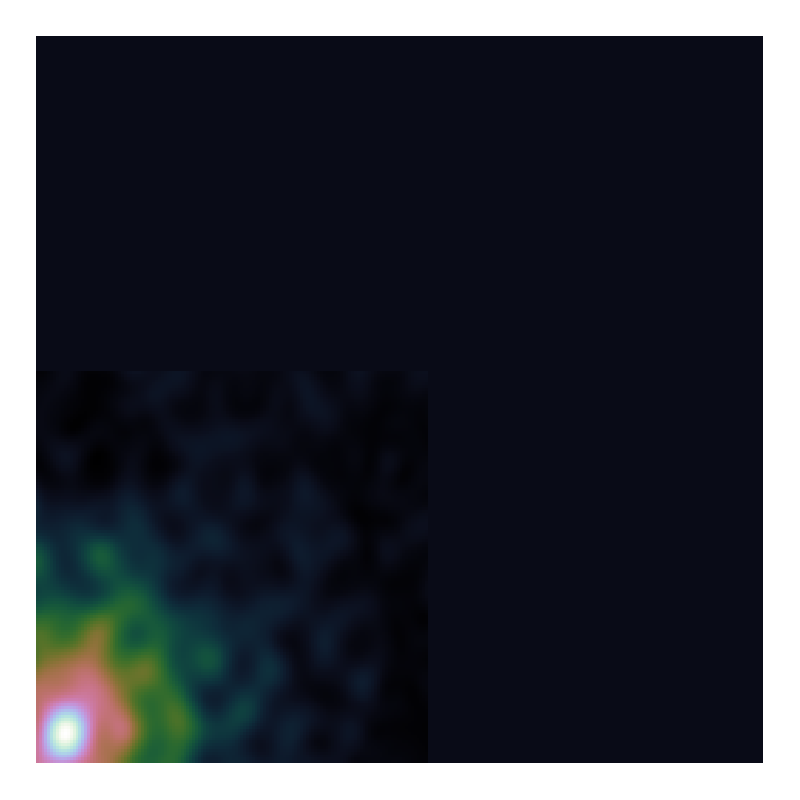
\includegraphics[width=\linewidth, clip, trim= 0.25in 0.25in 0.25in 0.25in]{./chapters/03.cd/simulated/psfZeroPadding.png}
		\caption{Zero padded convolution.}
		\label{cd:efficient:convolution:padded}
	\end{subfigure}
	\begin{subfigure}[b]{0.3\linewidth}
		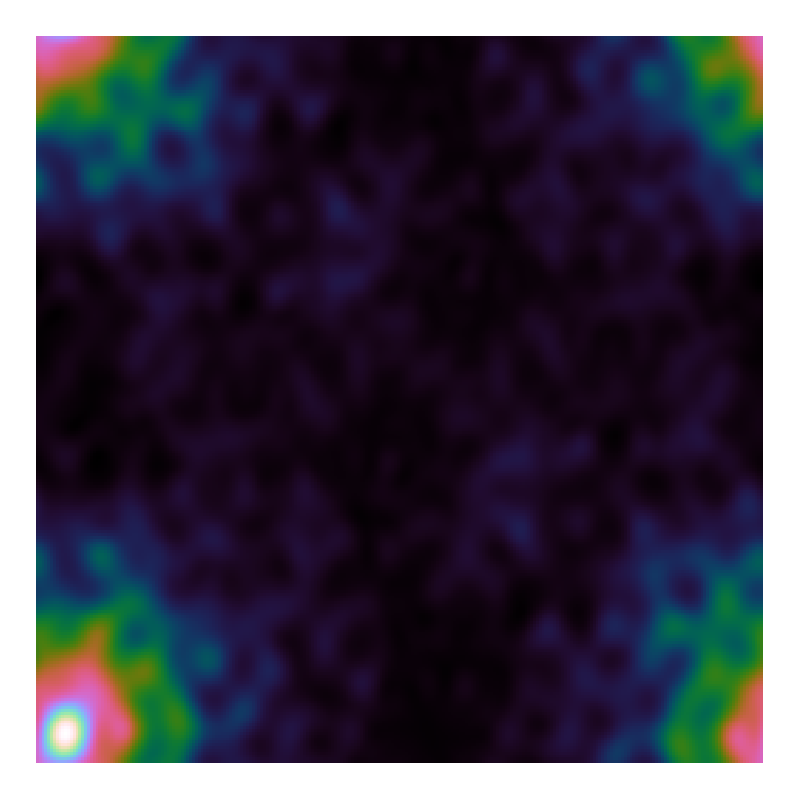
\includegraphics[width=\linewidth, clip, trim= 0.25in 0.25in 0.25in 0.25in]{./chapters/03.cd/simulated/psfCircular.png}
		\caption{Circular convolution.}
		\label{cd:efficient:convolution:circular}
	\end{subfigure}
	\caption{Comparison of the two convolution schemes.}
	\label{cd:efficient:convolution:figure}
\end{figure}

Circular convolution assumes the image "wraps" around itself. If we travel over the right edge of the image, we arrive at the left edge. The convolution in Fourier space is circular. Remember: A convonlution in image space is a multiplication in Fourier space, and vice versa. When we convolve the reconstructed image $x$ with the $PSF$ using circular convolution, then non-zero pixels at the right edge of the image "shine" over to the left edge. This is physically impossible.

Zero padding assumes that after the edge, the image is zero. Non-zero pixels at the right edges of the image do not influence the left edge after convolution. This is the physically plausible solution. However, the zero padded convolution is more expensive to calculate. We either have to calculate the convolution in image space, which is too expensive for large kernels, or apply the FFT on a zero-padded image. Either way, it is more expensive than the circular convolution.

In designing a deconvolution algorithm, we have the choice between the circular and the zero-padded convolution scheme. Circular convolution is more efficient to calculate, while zero-padded convolution is closer to the reality. Both choices are possible. Some implementations leave this choice to the user \cite{kenyon2019pymoresane}. We decide on using the zero-padded convolution. This choice influences how we calculate the Lipschitz and gradients efficiently.


\subsubsection{Using a map of gradients}
For an efficient greedy strategy, we need to know the gradient for each pixel.  We show how to calculate the initial map of gradients efficiently with the FFT, and how to update it directly after a change in the reconstructed image $x$. As we will see, we can use a map of gradients and drop the residual image from the algorithm. The gradient map implicitly contains the information of the residuals.

\textbf{Efficient initialization }\\
Calculating the gradient for each pixel results again in a quadratic runtime. We need to calculate $\langle residuals, PSF_{location} \rangle$ for every pixel. But we can use the FFT to efficiently calculate the map of gradients in time. Note that the inner product is actually a correlation: We correlate the $PSF$ with the residuals. The correlation and the convolution are related. The convolution is simply a correlation with a flipped kernel. This means we can use the $FFT$ to efficiently calculate the correlation of the residuals and the $PSF$:

\begin{equation}\label{cd:efficient:gradients:correlation}
\begin{split}
psfFlipped &= FlipUD(FlipLR(PSF)) \\
gradients &= iFFT(FFT(residuals) * FFT(psfFlipped))
\end{split}
\end{equation}

A convolution in image space is a multiplication in Fourier space. This fact can also be exploited for the correlation by flipping the $PSF$. Since the FFT takes linearithmic time $O(n log n)$ to compute, the overall operation also takes us linearithmic time. The operation is shown in Figure \ref{cd:efficient:gradients:figure}.

\begin{figure}[h]
	\centering
	\begin{subfigure}[b]{0.3\linewidth}
		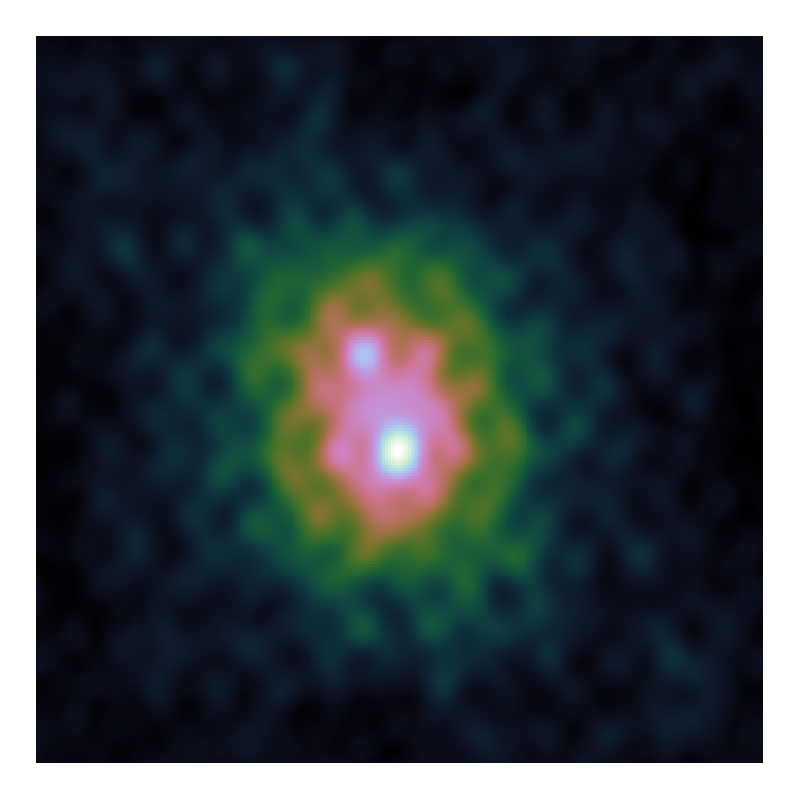
\includegraphics[width=\linewidth, clip, trim= 0.25in 0.25in 0.25in 0.25in]{./chapters/03.cd/simulated/dirty.png}
		\caption{Dirty Image.}
		\label{cd:efficient:gradients:dirty}
	\end{subfigure}
	\begin{subfigure}[b]{0.3\linewidth}
		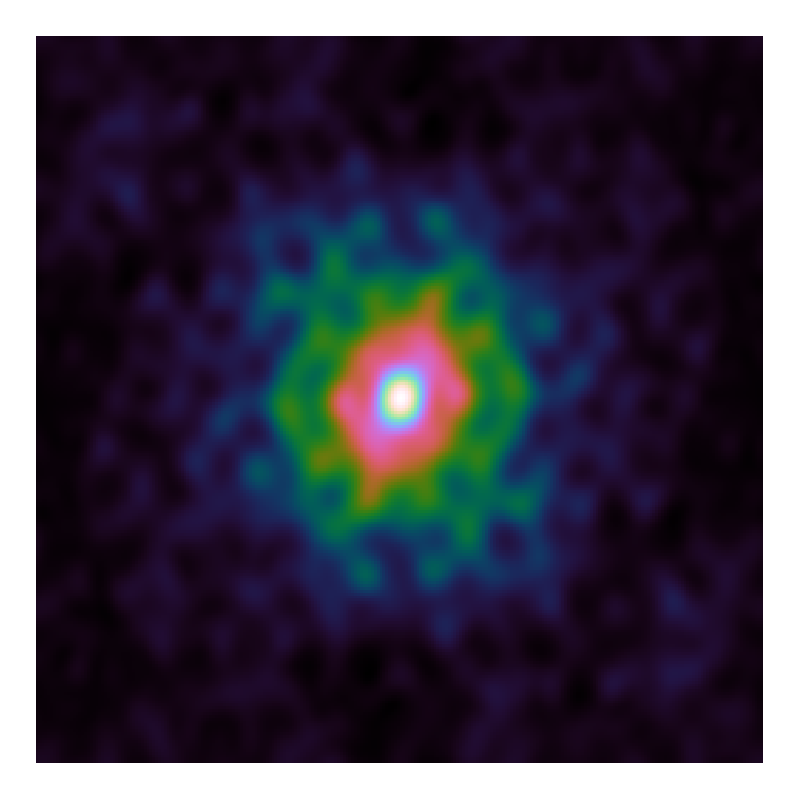
\includegraphics[width=\linewidth, clip, trim= 0.25in 0.25in 0.25in 0.25in]{./chapters/03.cd/simulated/psf.png}
		\caption{Point Spread Function.}
		\label{cd:efficient:gradients:psf}
	\end{subfigure}
	\begin{subfigure}[b]{0.3\linewidth}
		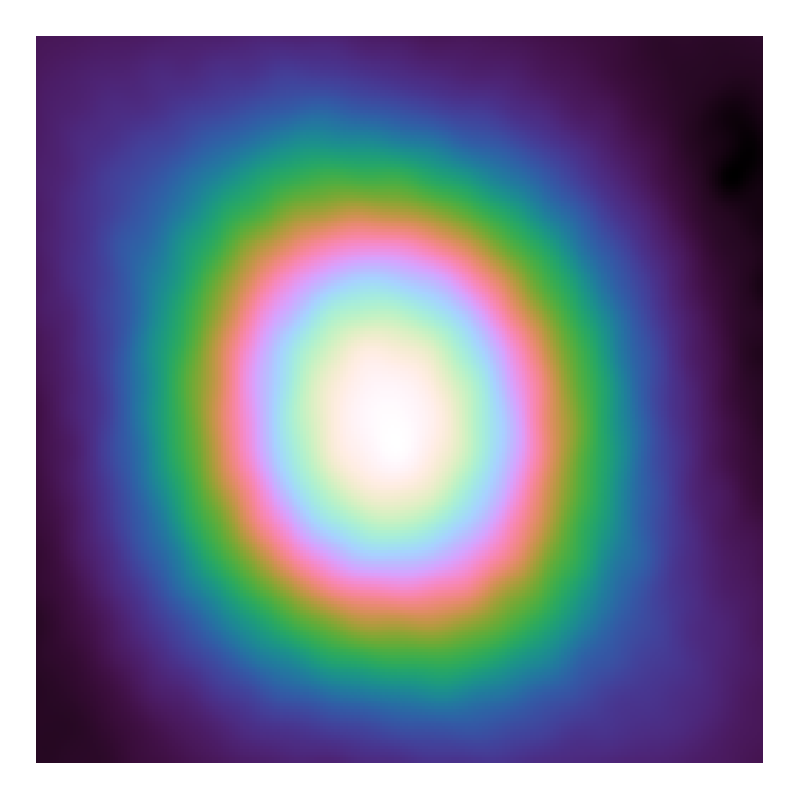
\includegraphics[width=\linewidth, clip, trim= 0.25in 0.25in 0.25in 0.25in]{./chapters/03.cd/simulated/gradients.png}
		\caption{Gradient map.}
		\label{cd:efficient:gradients:gradients}
	\end{subfigure}
	
	\caption{Example of the gradient calculation.}
	\label{cd:efficient:gradients:figure}
\end{figure}


\textbf{Direct update of gradient map}\\
Thanks to the FFT, we can efficiently calculate the map of gradients at the start of the serial coordinate descent algorithm. After we update a pixel in the reconstruction $x$, the map changes. We could repeat the correlation in the Fourier space from equation \eqref{cd:efficient:gradients:correlation} at each iteration. But this is wasteful. We can update the map of gradients directly.

Note that if we add pixel in the reconstruction $x$, we subtract the $PSF$ (multiplied with the pixel value) from the specific location in the residuals. The gradient map is then calculated by again correlating the $PSF$ with the residuals. We update the residuals by subtracting the $PSF$ at the correct location. And we update the gradient map by subtracting the $PSF$ correlated with itself at the correct position ($PSF \star PSF$). In our simulated example, the $PSF$ and the gradient update map is shown in Figure \ref{cd:efficient:update:psf}.
\begin{figure}[!h]
	\centering
	\begin{subfigure}[b]{0.3\linewidth}
		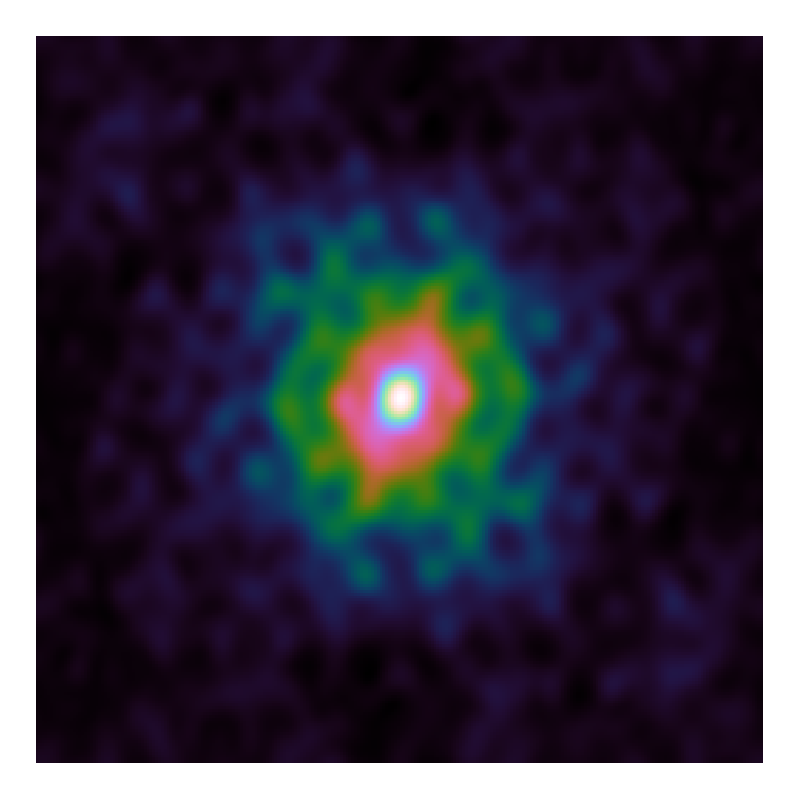
\includegraphics[width=\linewidth, clip, trim= 0.25in 0.25in 0.25in 0.25in]{./chapters/03.cd/simulated/psf.png}
		\caption{Point Spread Function.}
		\label{cd:efficient:update:dirty}
	\end{subfigure}
	\begin{subfigure}[b]{0.3\linewidth}
		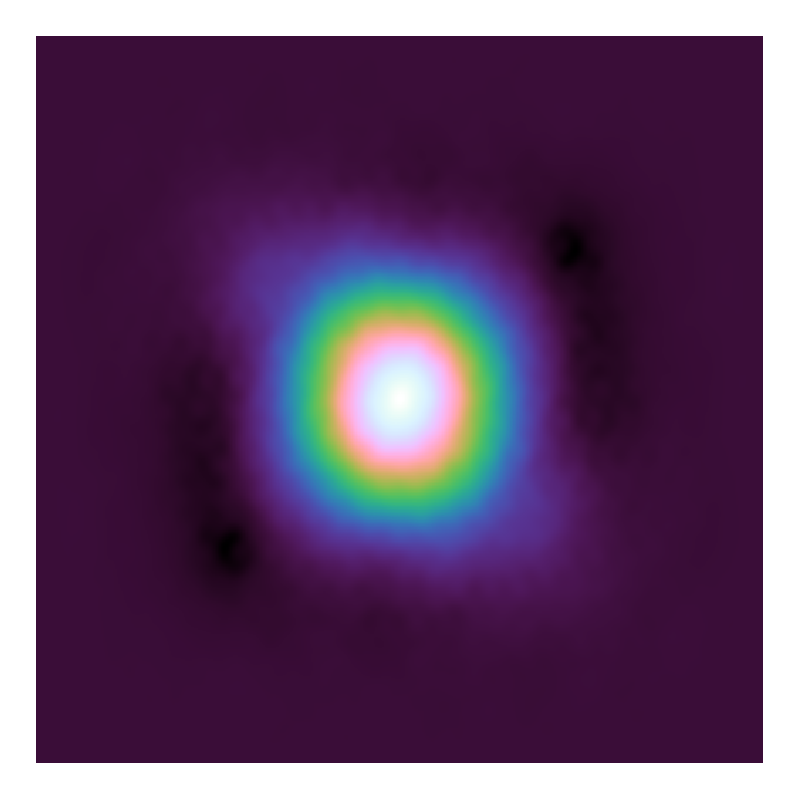
\includegraphics[width=\linewidth, clip, trim= 0.25in 0.25in 0.25in 0.25in]{./chapters/03.cd/simulated/psfSquared.png}
		\caption{Gradient update: $(PSF \star PSF)$.}
		\label{cd:efficient:update:psf}
	\end{subfigure}
	\caption{Example problem with two point sources.}
	\label{cd:efficient:update:figure}
\end{figure}

This means we can update the gradient map directly with the product of $(PSF \star PSF)$. We can simply shift $(PSF \star PSF)$ at the correct pixel location and subtract it from the gradient map directly. Although there is one issue: We use zero padded convolution. The $PSF$ at the edges of the image is masked. This means that the product $(PSF \star PSF)$ actually changes with the pixel location. If we update a pixel in the corner of the image, the actual update $(PSF \star PSF)$ at that location looks different than what was shown in Figure \ref{cd:efficient:update:psf}.

The exact update is again expensive to calculate. We need to shift the $PSF$ at its correct location and again calculate the correlation with itself. However, the exact gradient update only changes significantly at the edges of the image, when large parts of the $PSF$ are masked by the edges. Otherwise the difference between the exact update and simply shifting $(PSF \star PSF)$ at the pixel location is small. This is the reason why we chose to accept that the gradient update is only an approximation. The approximation only becomes inaccurate at the edges, and we use the algorithm in the Major cycle framework: Every Major cycle removes any inaccuracies we introduced during the previous cycle.  

\subsection{Efficient implementation pseudo-code}
Now we put all the run time improvements discussed before into the new implementation of the serial coordinate descent algorithm. We pre-calculate the Lipschitz constants and the gradient map. Then during iterations, we update the gradient map directly.

This leads to the following algorithm:
\begin{lstlisting}
dirty = IFFT(GridVisibilities(visibilities))
residualsPadded = ZeroPadding(dirty)

psfPadded = ZeroPadding(PSF)
psfPadded = FlipUD(FlipLR(psfPadded))
gradientUpdate = iFFT(FFT(ZeroPadding(PSF)) * FFT(psfPadded))

x = new Array[,]
gradientsMap = iFFT(FFT(residualsPadded) * FFT(psfPadded))
lipschitzMap = CalcLipschitz(PSF)

objectiveValue = 0.5* Sum(residuals * residuals) + ElasticNet(x)
maxAbsDiff = 0
do 
	oldObjectiveValue = objectiveValue
	
	//Step 1: Search pixel
	maxAbsDiff = 0
	maxDiff = 0
	pixelLocation = (-1, -1)
	for(i in Range(0, dirty.Length(0))
		for(j in Range(0, dirty.Length(1))
			oldValue = x[i, j]
			tmp = gradientsMap[i, j] + oldValue * lipschitzMap[i, j]
			optimalValue = Max(tmp - lambda*alpha) / (lipschitz[i, j] + (1 - alpha)*lambda)
			diff = optimalValue - oldValue
			
			if(maxAbsDiff < Abs(diff))
				maxAbsDiff = Abs(diff)
				maxDiff = diff
				pixelLocation = (i, j)
	
	//Step 2: Optimize pixel. Now all that is left is to add the maximum value at the correct location
	x[pixelLocation] += maxDiff
	
	//housekeeping
	shiftedUpdate = Shift(gradientUpdate, pixelLocation)
	gradientMap = gradientMap - shiftedUpdate * maxDiff
while epsilon < maxAbsDiff
\end{lstlisting}

In step 1, we replaced the gradient and Lipschitz calculation with lookups, reducing the runtime costs of the step. In this implementation, step 2 is trivial. We only need to update the reconstruction at the correct location. All the important work has already been completed in step 1.

The two most time consuming parts of this implementation are step 1, and updating the gradient map. Our implementation in .Net Core uses parallel computing for both parts. We search for the maximum pixel in parallel, and update the gradient map in parallel.


\subsection{Serial coordinate descent and similarities to the CLEAN algorithm}\label{cd:similarities}
When we look back at the CLEAN algorithm described in Section \ref{intro2:CLEAN}, we can see similarities in their structures: In the first step, CLEAN searches the location of the maximum pixel in the residuals, while serial coordinate descent searches the location of the absolute maximum change. In the second step, CLEAN subtracts a fraction of the $PSF$ at that location, while coordinate descent calculates the optimal pixel value and subtracts the product of $PSF \star PSF$ from the gradient map. 

CLEAN and serial coordinate descent have the same overall structure. But serial coordinate descent uses the gradient map instead of explicit residuals (the gradient map contains the information of the residuals implicitly). In a sense, the serial coordinate descent can be looked at as a CLEAN algorithm, which uses the gradient map instead of the residual map, and the product of $PSF \star PSF$ instead of the $PSF$. Both algorithms use essentially use the same operations, but the content in their memory is different. As such, one iteration of standard CLEAN is roughly as expensive as an iteration of serial coordinate descent. 

The side effect of their similar structure is that any speedup we achieve by using GPU acceleration for serial coordinate descent can plausibly be used to speedup CLEAN to a similar amount. Our distribution scheme for serial coordinate descent can also be used for a distributed standard CLEAN. 

The main difference between the two algorithms is that serial coordinate descent does not need the blurring step typically used in CLEAN algorithms. In Section \ref{intro2:CLEAN}, we introduced the CLEAN concept of the model image. Standard CLEAN detects point sources, and puts them in the model image. When the observation shows an extended emission, the standard CLEAN approximates it as a set of point sources. After CLEAN has finished finding all the point sources, it blurs the model image with the clean-beam, a 2d Gaussian representing the accuracy of the instrument, resulting in the reconstructed image.

In this project, we use the elastic net regularization, which has a simple model for extended emissions, namely the L2 norm. As such our serial coordinate descent algorithm can find the reconstructed image directly without any blurring. This may result in super-resolved reconstructions: The serial coordinate descent algorithm may find structures which are smaller than the accuracy limit of the instrument. We will show plausible super-resolved reconstructions by the serial coordinate descent algorithm with elastic net regularization in Section \ref{results}.

%Multi-scale CLEAN is what is used. Difficulty with MPI implementation because of a distributed convolution.


\newpage
\section{Gradient/PSF approximation for distributed deconvolution} \label{gradients}

Distributed deconvolution, we would like to deconvovle patches of the final image independently from each other. 
Concept of seperability. Number of non-zero components.

The size of the $PSF$ tells us how far the patches have to be apart from each other to be independent.
Limiting factor for distribution is the size of the $PSF$. We would like to deconvolve pixels, or patches of the image independently from each other. But the $PSF$ does not let us do that. As soon as the $PSF$ overlap, they are not independent anymore.
Generally the $PSF$ spans over the whole image. 

But the $PSF$ for MeerKAT is peculiar.
In the center, the $PSF$ approximates a Gaussian function, which spans only over a fraction of the image. Indeed, with increasing number of visibility measurements, the $PSF$ becomes more and more like a Gaussian function.
Also, the values of the $PSF$ become smaller the further we walk away from the center. Although the $PSF$ spans over the whole image, its values become insiginificant.

MeerKAT has wide field of view observations with an increasingly Gaussian-like $PSF$. Can we use the significant fraction of the $PSF$ instead? Is this enough?
We have two operations, calculating the gradients of the image, and updating the gradients.
View of stochastic gradient descent. So if we calculate the gradient of a pixel with $-2 \langle residuals, PSF \rangle$, then we should be able to approximate the gradient with only a fraction fo the $SF$. But the pre-calculation of gradients is actually cheap, the thing. But what about updating the gradients?
We


Also,
Plus the major cycle framework: It already corrects for the fact that the $PSF$ we use is only an approximation of the true $PSF$. $w$-term changes the $PSF$ over the image. 



The answer to this is yes, we can. In Section \ref{results:gradients} we demonstrate the speedup of the deconvolution with only a fraction of the $PSF$ on a real world MeerKAT dataset. In this Section, we show how this can be done. 



The problem is arriving at the same optimum. Not trivial.



\subsection{Difficulty in approximating the $PSF$}

In our coordinate descent deconvolution, we use the $PSF$ in two steps. Before we run coordinate descent, we pre-calculate the gradient for each pixel with a correlation operation. During coordinate descent deconvolutions, we update the gradient-map directly. Two opposing solutions: We use the full $PSF$ to pre-calculate the gradients, but only update the gradients with a fraction of the $PSF$. That way we always start from the correct gradients, but get less accurate over coordinate descent deconvolutions.

\subsection{Approximate gradient update}

So we use the full $PSF$

only update with a fraction of the $PSF$

$PSF$ squared update. Scaling.
So we become less and less accurate


\subsection{Approximate deconvolution}

We never use the full PSF

But the problem of gradient magnitude. 

Change lambda. We do an approximate deconvolution. 


\subsection{Major Cycle convergence}
\cite{clark1980efficient} and the question on how many iterations per major cycle
Putting it all together

We have the Minor Cycle, which is easy to converge.

Coordinate Descent Path optimization \cite{friedman2010regularization}
Danger that CD takes too many pixel into a Major Cycle. Lower bound per iteration, PSF sidelobe
can still be too low, danger when many psf sidelobes overlap
\newpage
\section{Tests on MeerKAT LMC observation}\label{results}
The Large Magellanic Cloud (LMC) is a galaxy is the second or third closest galaxy to the Milky Way. Figure \ref{results:LMC} shows the LMC in both optical and radio wavelenghts. The radio wavelengths was observed by the VLA radio interferometer\cite{bock1999sumss} at 843MHz. In the optical wavelengths, the abundance of stars are clearly visible. The LMC is close enough to earth for individual stars are visible. But it also contains a large number of supernova remnants, gas clouds, and other extended emissions, which shine bright in the radio wavelengths.
 
The LMC is a region with a large number of sources at different brightness. In the lower-right quadrant of the radio-image \ref{results:LMC:radio}, we see the bright emission of the supernova remnant N132D, the brightest radio source in the LMC. But around the N132D are faint emissions from gas-clouds. This means faint emissions may get lost next to N132D. We need a deconvolution algorithm to uncover these faint emissions.
 
We received a MeerKAT observation of the LMC from SARAO for the purpose of algorithm testing. At the time of writing, the MeerKAT instrument is still being tested. The observation is only representative in the data volume. The observation is calibrated, and averaged down in both frequency and time. The averaging reduces both the disk space and the runtime costs of the gridding step. Nevertheless, the observation takes up over 80 GB of disk space (roughly $\frac{1}{30}$ of the original data). A CLEAN reconstruction of the calibrated observation is shown in Figure \ref{results:LMC:meerkat}.
 
\begin{figure}[h]
	\centering
	\begin{subfigure}[b]{0.3\linewidth}
		\includegraphics[width=1.0\linewidth]{./chapters/10.results/LMC/optical_cut.png}
		\caption{Optical wavelength}
	\end{subfigure}
	\begin{subfigure}[b]{0.30\linewidth}
		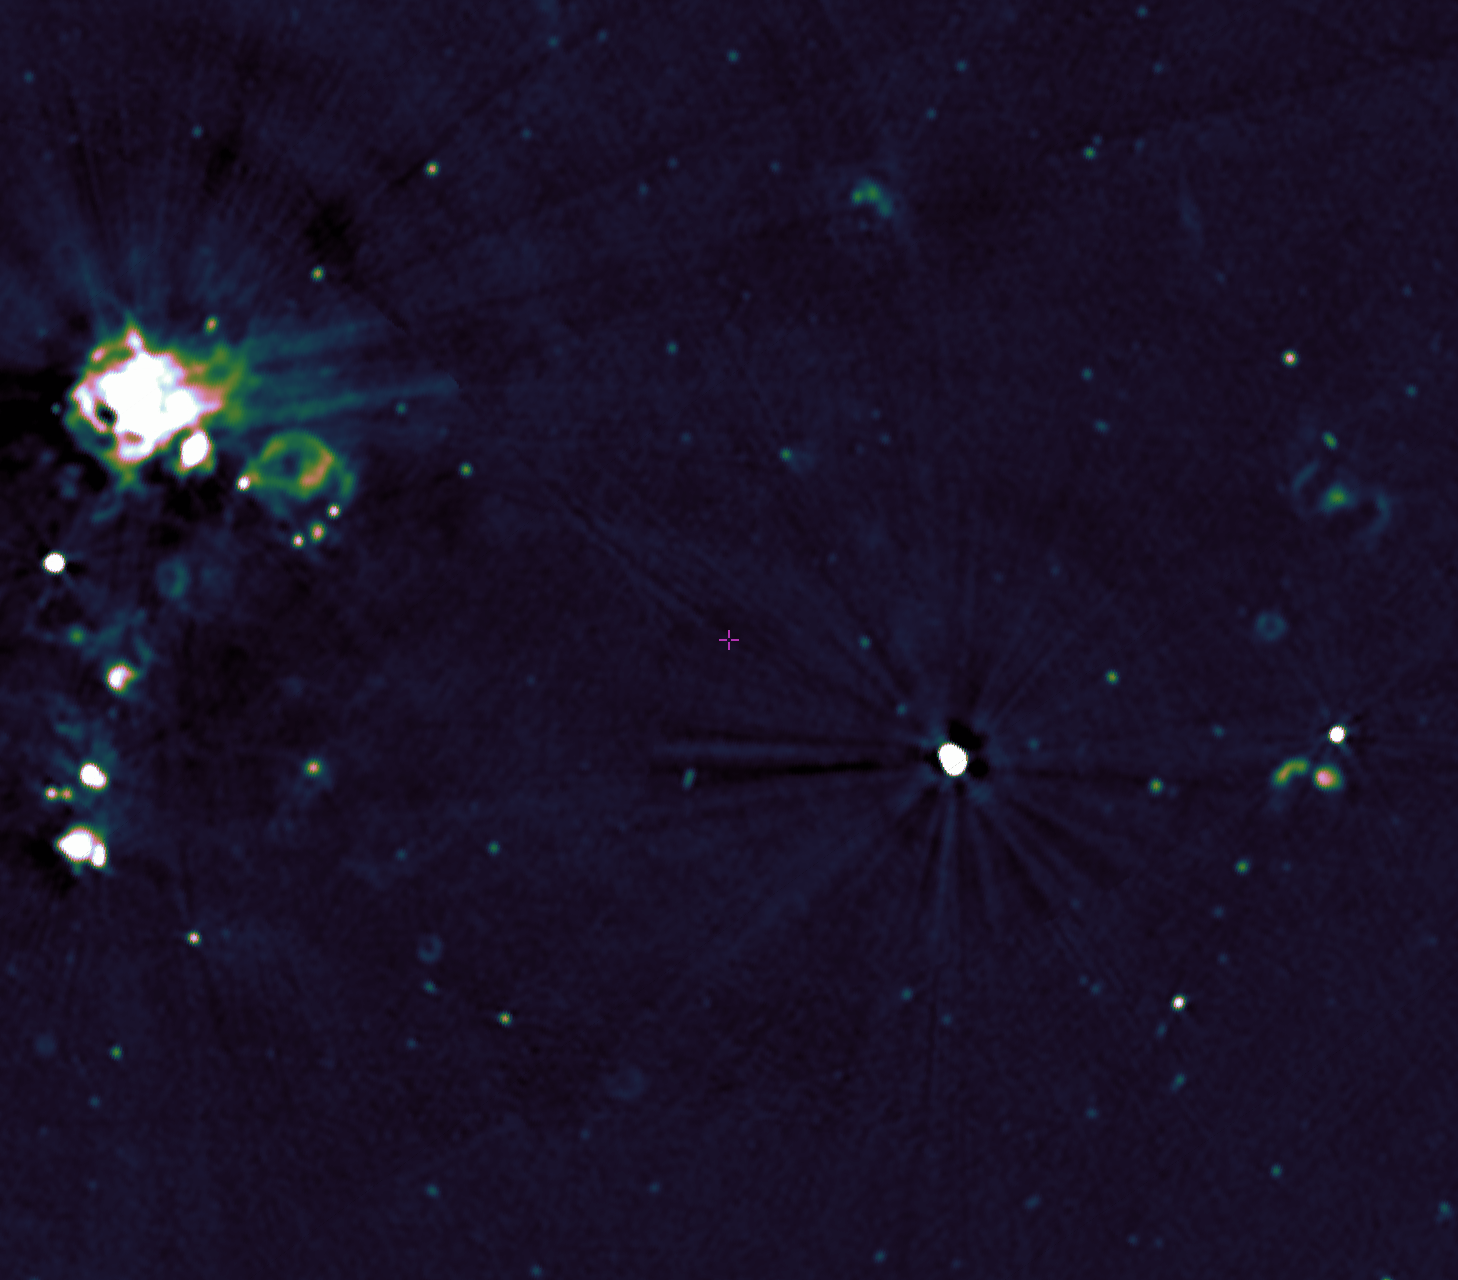
\includegraphics[width=1.0\linewidth]{./chapters/10.results/LMC/radio-843_cut.png}
		\caption{Radio wavelength at 843MHz.}
		\label{results:LMC:radio}
	\end{subfigure}
	\begin{subfigure}[b]{0.375\linewidth}
		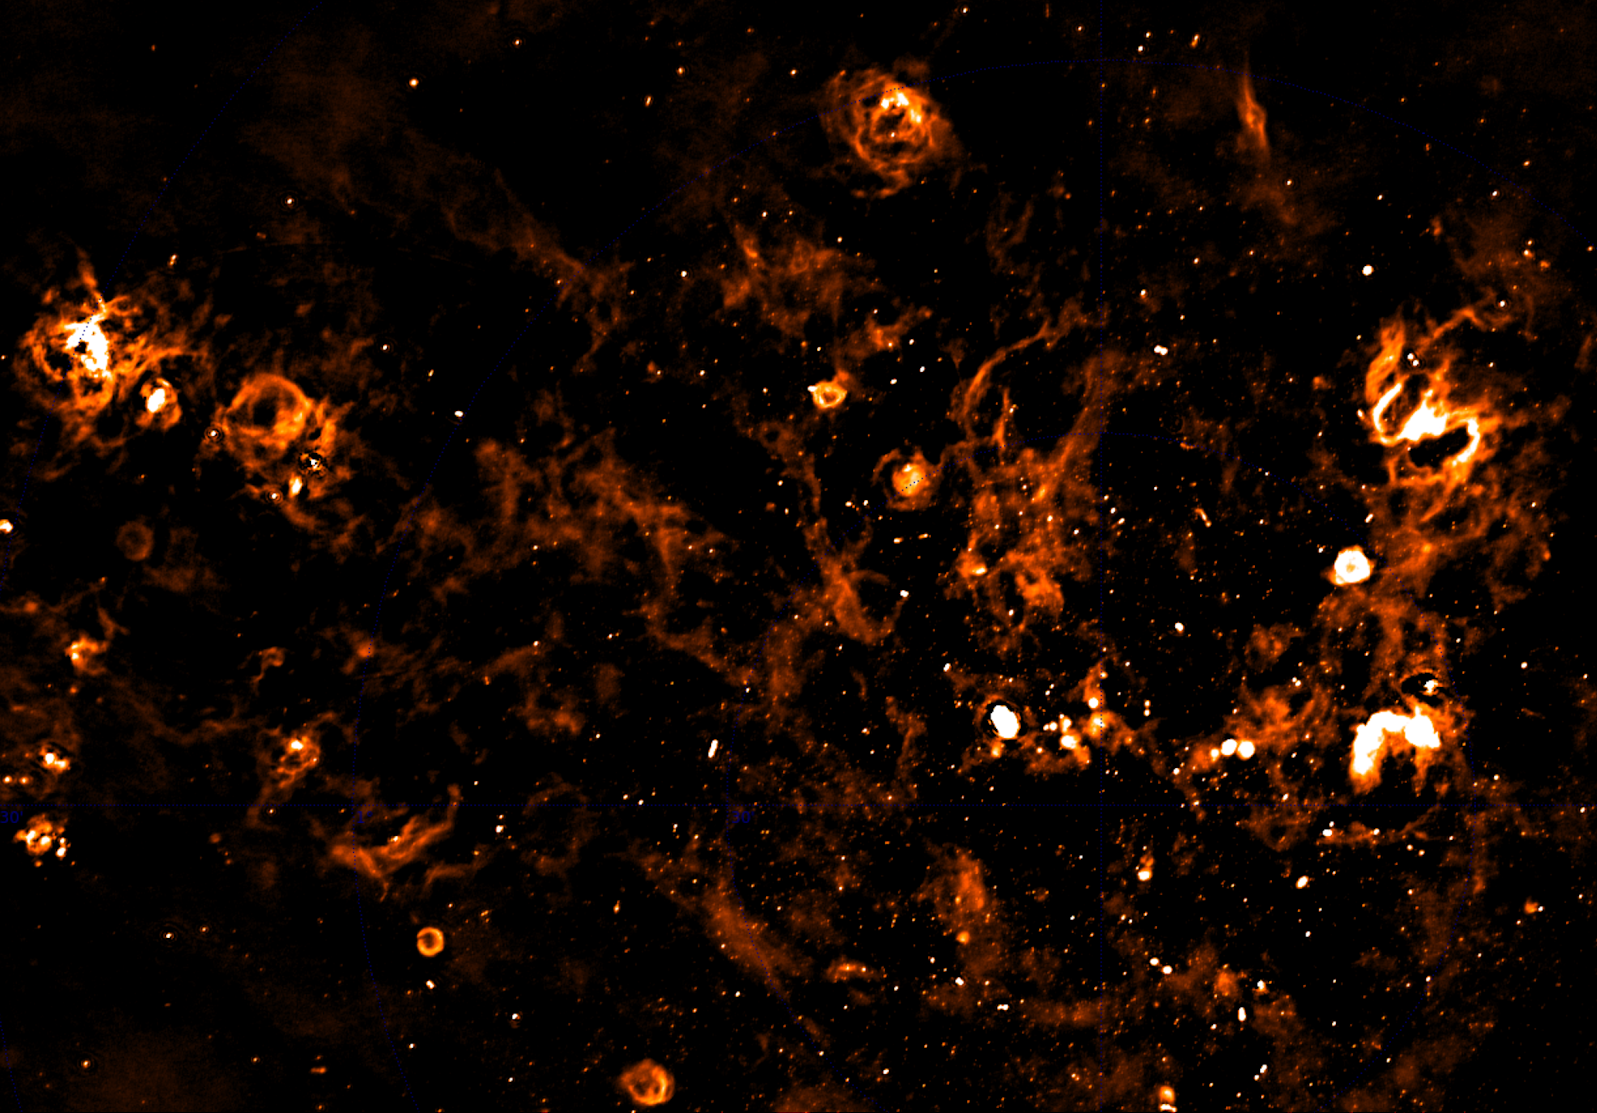
\includegraphics[width=1.0\linewidth]{./chapters/10.results/LMC/meerkat2.png}
		\caption{Wide band radio image by MeerKAT.}
		\label{results:LMC:meerkat}
	\end{subfigure}
	\caption{Section of the Large Magellanic Cloud (LMC)}
	\label{results:LMC}
\end{figure}

The MeerKAT observation covers a wide band of radio frequencies. The lowest frequency in the MeerKAT observation is 894 MHz, and the highest frequency is
Imaging the whole frequency band requires a wide band deconvolution algorithm. In wide band imaging, several images at different frequencies get deconvolved as an image cube. Wide band imaging again multiplies the amount of work that has to be done for reconstruction, as now we cannot deconvolve a single image, but have to deal with a whole image cube.

Wide band imaging is not possible within the time frame of this project. We take a narrow band subset of 5 channels from the original data (ranging from 1084 to 1088 MHz, about 1 Gb in size) for reconstruction. We also reduce the field-of-view to a more manageable section. Figure \ref{results:cutout} shows the LMC image section we are using together with a CLEAN reconstruction of the narrow band data.

\begin{figure}[h]
	\centering
	\begin{subfigure}[b]{0.4\linewidth}
		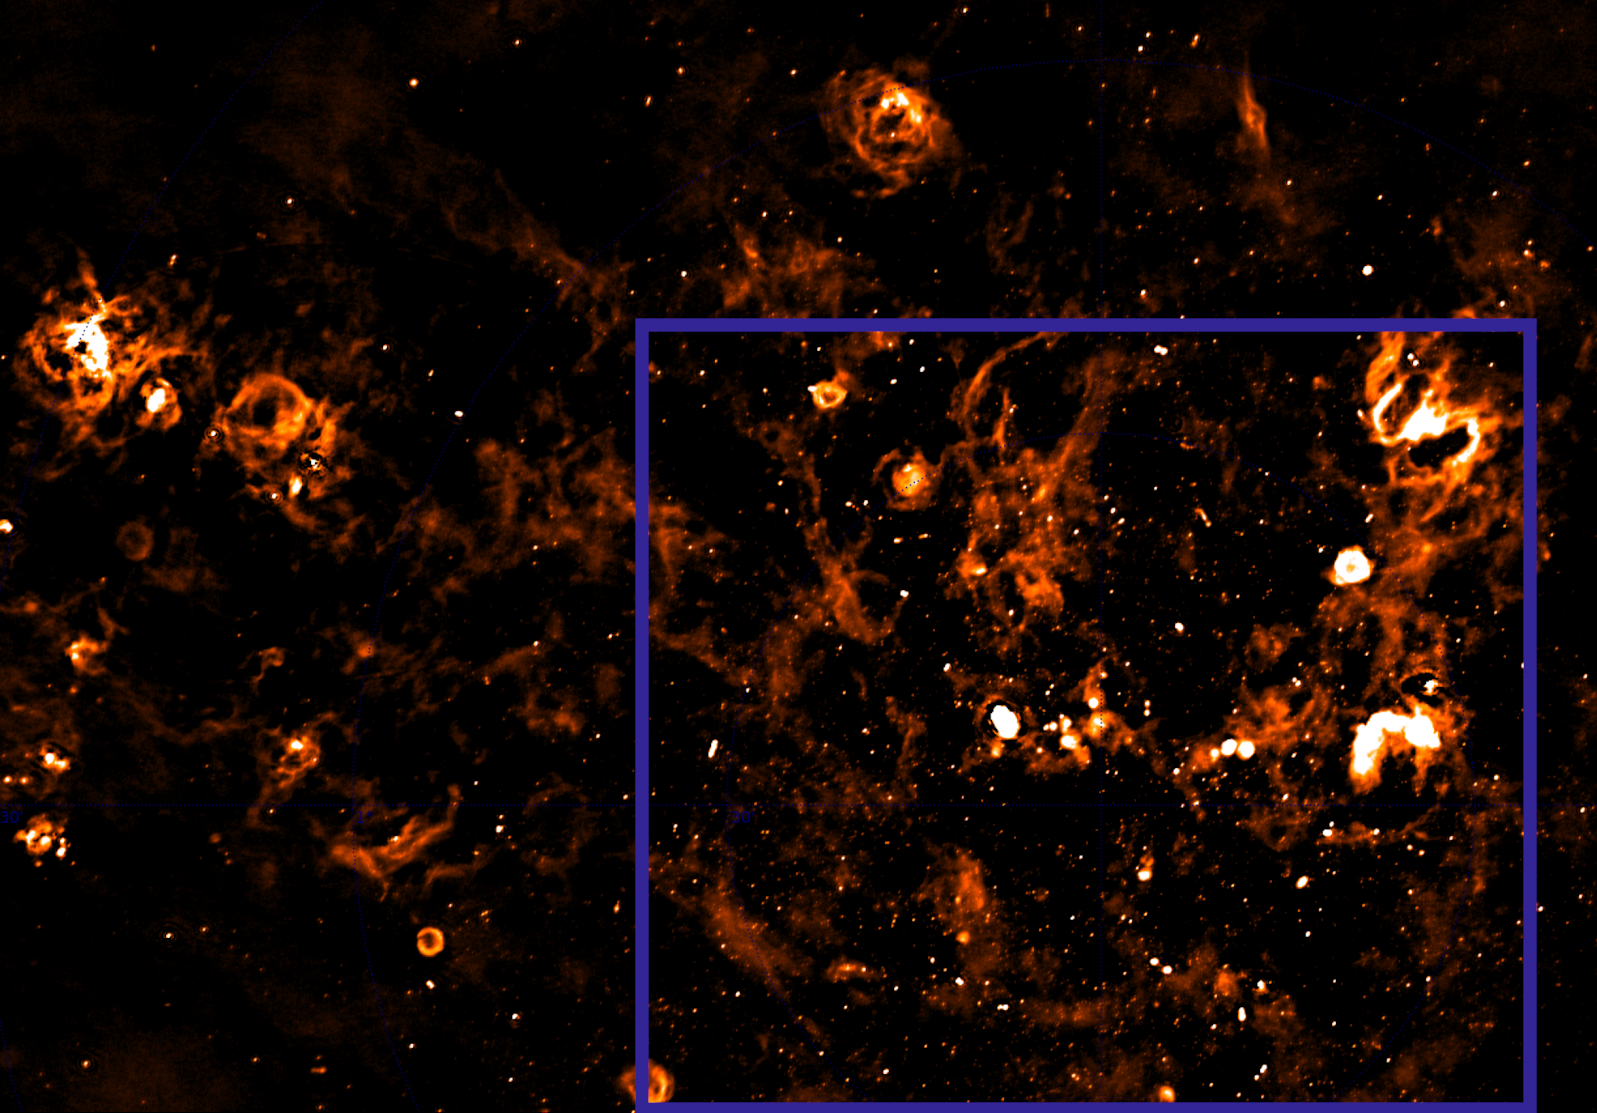
\includegraphics[width=1.0\linewidth]{./chapters/10.results/LMC/meerkat_cutout.png}
	\end{subfigure}
	\begin{subfigure}[b]{0.30\linewidth}
		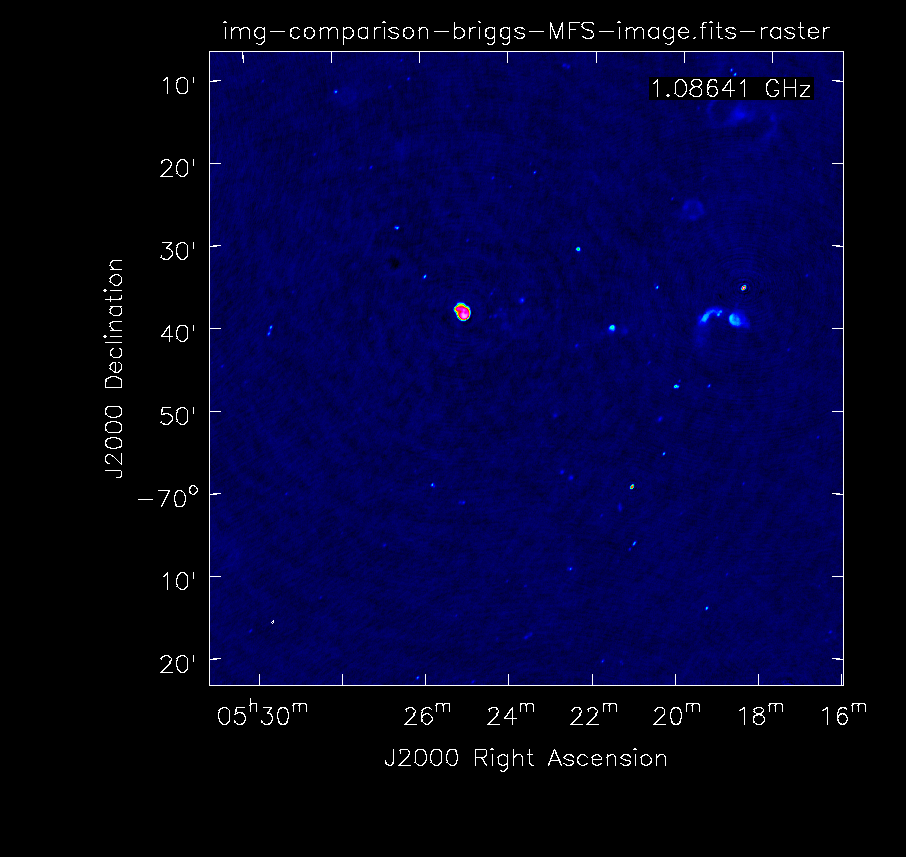
\includegraphics[width=1.0\linewidth]{./chapters/10.results/cleancomp/clean_briggs.png}
	\end{subfigure}
	\caption{Narrow band image section used.}
	\label{results:cutout}
\end{figure}

At the center of our image section \ref{results:cutout} we see the N132D supernova remnant. We partially see the faint extended emissions, although they are close to the noise level. This is known as a high-dynamic range reconstruction. We have strong radio sources mixed together with faint emissions, which are only marginally above the noise level of the image.

The total field-of-view of our image section is roughly 1.3 degrees(or 4600 arc seconds). Our reconstruction has $3072^2$ pixel with a resolution of 1.5 arc seconds per pixel. this is still a wide field-of-view reconstruction problem. We have to account for the effects of the $w$-term to achieve a high-dynamic range reconstruction.

In our test reconstruction, we need to account for $w$-term correction and high-dynamic range. We have excluded wide-band imaging as not feasible within the time frame of this project. In Section \ref{results:cleancomp} we compare the reconstructions of CLEAN with our coordinate descent based algorithm on the LMC observation. The next Section \ref{results:speedup} presents the speedup we achieve with coordinate descent by using our distributed or GPU-accelerated implementations.

In Section \ref{results:gradients} we show the core result of this project. Namely what effect has an approximate $PSF$ on the deconvolution problem and whether we can use it to further distribute the problem. The answer to that question is affirmative: We can approximate the $PSF$, and we can exploit it to further distribute the deconvolution. But we need more sophisticated coordinate descent algorithms to fully benefit from it.


\subsection{Comparison with CLEAN reconstructions} \label{results:cleancomp}
We use the WSCLEAN \cite{offringa2014wsclean} implementation of multi-scale CLEAN. We compare our coordinate descent reconstruction with two CLEAN reconstructions, oe with naturally weighted visibilities and one with briggs weighted visibilities.

There are three main visibility weighting scheme for the gridder that lead to different $PSF$s from the same measurements: Natural, uniform, and Briggs\cite{briggsWeighting}. Natural weighting scheme leads to an image with a lower noise level, but a wider $PSF$. Uniform weighting leads to a higher noise level, but to a $PSF$ whgich is more concentrated around a single pixel. Briggs weighting is a scheme combines the best from both worlds, receiving an image with acceptable noise level while getting a more concentrated $PSF$. As such it is widely used in radio astronomy image reconstruction. Our gridder implements the natural weighting scheme only. Nevertheless our coordinate descent algorithm is able to retrieve structures similar to the briggs-weighted multi-scale CLEAN reconstruction, even though coordinate descent has to work with a wider $PSF$.

\begin{figure}[h]
	\centering
	\begin{subfigure}[b]{0.4\linewidth}
		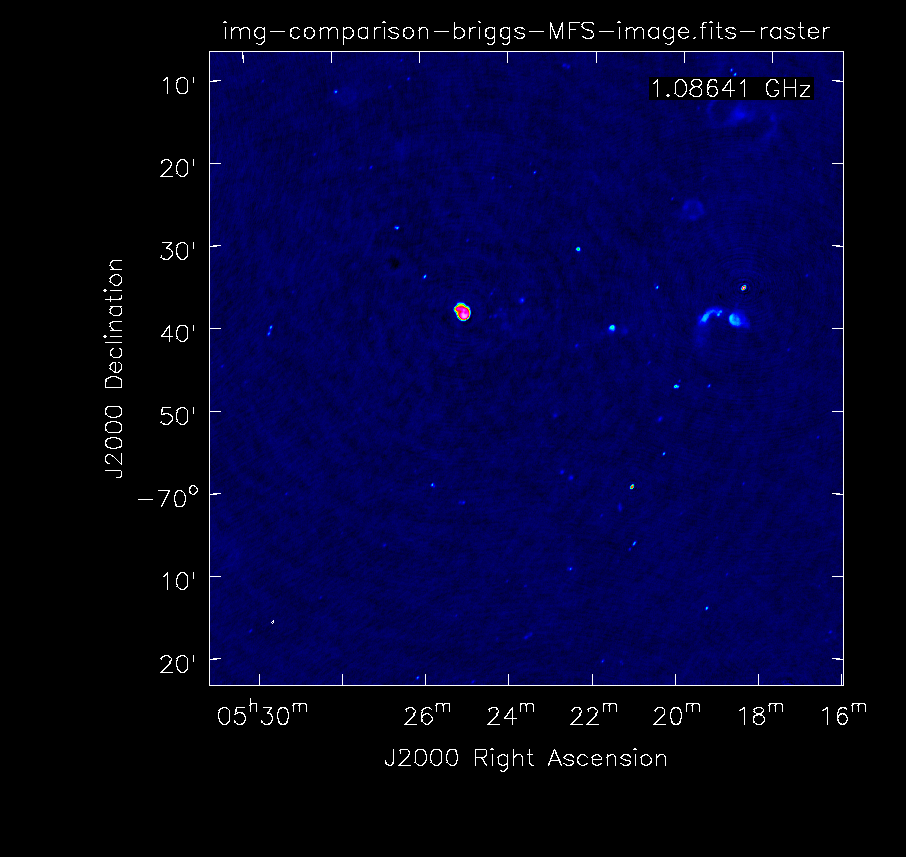
\includegraphics[width=1.00\linewidth]{./chapters/10.results/cleancomp/clean_briggs.png}
		\caption{Briggs weighted multi-scale CLEAN.}
		\label{results:comp:clean}
	\end{subfigure}
	\begin{subfigure}[b]{0.40\linewidth}
		\includegraphics[width=1.00\linewidth]{./chapters/10.results/cleancomp/cd.png}
		\caption{Naturally weighted coordinate descent.}
		\label{results:comp:cd}
	\end{subfigure}
	\caption{Comparison of the whole image}
	\label{results:cleancomp:figure}
\end{figure}

Figure \ref{results:cleancomp:figure} shows the reconstruction of both briggs-weighted multi-scale CLEAN and the naturally weighted coordinate descent reconstruction.
%parameters for CLEAN and Coordinate descent. Lambda and alpha
CLEAN used 6 major cycles and 14 thousand minor cycle iterations. Our coordinate descent implementation converged after 5 major cycles and needed 100 thousand iterations to converge.

Coordinate descent needs a large number of iterations to converge when compared to multi-scale CLEAN. Note that a coordinate descent iteration is cheaper to compute than one iteration of multi-scale CLEAN. Also note that because we are searching for structures close to the noise level of the image, coordinate descent often adds pixels belonging to the noise in one major cycle, just to remove them in the next one. Path regularization\cite{friedman2010regularization} can combat this problem, and gets further investigated in the following Section \ref{results:gradients}.

Both algorithms detect the three extended emissions at the right side of the image. They detect various point sources at the same location. Coordinate descent and multi-scale CLEAN arrive at a roughly similar result. Coordinate descent detects similar structures in the N132 supernova remnant, as the briggs-weighted CLEAN, but also includes calibration errors in its reconstruction of the faint extended emissions.

\begin{figure}[h]
	\centering
	\begin{subfigure}[b]{0.3\linewidth}
		\includegraphics[width=1.00\linewidth]{./chapters/10.results/cleancomp/n132_clean.png}
		\caption{CLEAN Natural weighting.}
		\label{results:N132:clean}
	\end{subfigure}
	\begin{subfigure}[b]{0.3\linewidth}
		\includegraphics[width=1.00\linewidth]{./chapters/10.results/cleancomp/n132_clean_briggs.png}
		\caption{CLEAN Briggs weighting.}
		\label{results:N132:cleanbriggs}
	\end{subfigure}
	\begin{subfigure}[b]{0.3\linewidth}
		\includegraphics[width=1.00\linewidth]{./chapters/10.results/cleancomp/n132_cd.png}
		\caption{CD Natural weighting.}
		\label{results:comp:N132:cd}
	\end{subfigure}
	\caption{N132 comparison}
	\label{results:cleancomp::N132:figure}
\end{figure}

Figure \ref{results:cleancomp::N132:figure} compares the naturally-weighted CLEAN, briggs CLEAN and coordinate descent on the N132 supernova remnant. The naturally-weigted CLEAN and coordinate descent use the same $PSF$ for the deconvolution. But coordinate descent finds structures in N132 similar to the briggs-weighted CLEAN. Coordinate descent arrived at a plausible higher-resolved reconstruction of N132.

\begin{figure}[h]
	\centering
	\begin{subfigure}[b]{0.3\linewidth}
		\includegraphics[width=1.00\linewidth]{./chapters/10.results/cleancomp/clean_calibration.png}
		\caption{Briggs CLEAN}
	\end{subfigure}
	\begin{subfigure}[b]{0.3\linewidth}
		\includegraphics[width=1.00\linewidth]{./chapters/10.results/cleancomp/cd_calibration.png}
		\caption{Coordinate Descent}
	\end{subfigure}
	\caption{Influence of calibration errors}
	\label{results:cleancomp::calib:figure}
\end{figure}

Calibration errors on the other hand negatively influence the coordinate descent reconstruction. Figure \ref{results:cleancomp::calib:figure} shows a cutout of the right hand section of the reconstruction, where a faint extended emission is next to a point source with calibration errors. Multi-scale CLEAN is able to differentiate between the "ripples" from the calibration error, and the signal from the extended emission. Coordinate descent with the elastic net regularization includes the ripples into the reconstructed image. 

The only way to exclude the ripples from the reconstruction is to increase the regularization parameter $\lambda$., such as no pixel gets included which is not above the noise level + calibration error in the image. However, that would lead to other sources being "regularized away" in other regions of the image, which do not have a severe calibration error close by. 


Case of super resolution.
Our coordinate descent algorithm works. All the performance optimizations do not break anything vital.


\subsection{Coordinate descent acceleration with MPI or GPU}\label{results:speedup}
Describe hardware

Distributed with MPI

GPU implementation

Measurement of the speedup.

\begin{figure}[h]
	\centering
		\begin{subfigure}[b]{0.4\linewidth}
		\includegraphics[width=1.00\linewidth]{./chapters/10.results/speedup/gpu.png}
	\end{subfigure}
	\begin{subfigure}[b]{0.4\linewidth}
		\includegraphics[width=1.00\linewidth]{./chapters/10.results/speedup/gpu.png}
	\end{subfigure}
	\caption{Speedup by using MPI or GPU acceleration}
	\label{results:speedup:figure}
\end{figure}


We cannot use MPI combined with the GPU. The MPI implementation uses a communication step in each coordinate descent iteration (communicating which pixel to optimize with MPI Allreduce). 



\subsection{Effect of approximating the $PSF$} \label{results:gradients}
As we described in Section \ref{gradients}, the $PSF$ for deconvolution is as big as the image. For wide field-of-view observations of MeerKAT, the $PSF$ is approximately a gaussian with decreasing pixel values the further we move from the center. Most of the values in the $PSF$ are close to zero. The question is, what effect has an approximate deconvolution with a smaller $PSF$? If we can approximate the deconvolution with a small enough $PSF$, we can solve patches of the image independently of each other. However, the $PSF$ approximation may need more major cycles to converge.

The effect of approximating the $PSF$ are not clear. We know that thanks to the $w$-term in the visibilities, the $PSF$ is not constant over the image. We already need several major cycles to converge. With a good approximation of the $PSF$, we may speed up the individual iterations of coordinate descent without needing more major cycle.

We presented two methods to approximating the $PSF$ for the deconvolution in Section \ref{gradients}. Method 1 updates only a fraction of the gradients, and Method 2 uses a fraction of the $PSF$ for deconvolution. We test both methods on the LMC data and explore what effects the approximations have on the reconstruction.

\subsubsection{Method 1: Approximate gradient update}
Our coordinate descent method updates the map of gradients after each iteration. This method only updates the most significant fraction of the gradients.
Method 1 starts with the same map of gradients as the original, but then only updates a fraction of the gradients in each iteration. It updates a rectangle of the most significant gradients.
With each iteration, the map of gradients gets less accurate. With enough major cycles, this method converges to the same optimum as the original coordinate descent method.

At the beginning of each major cycle, we calculate the objective value of the current solution. We compare the objective value and the wall-clock time of the original and the approximate gradient update. 
Target: get the lowest possible objective value.
Figure \ref{results:gradients:update} shows the results.

\begin{figure}[h]
	\centering
	\begin{subfigure}[b]{0.7\linewidth}
		\includegraphics[width=\linewidth]{./chapters/10.results/gradient/ApproxUpdate/size.png}
	\end{subfigure}
	\\
	\begin{subfigure}[b]{0.35\linewidth}
		\includegraphics[width=\linewidth]{./chapters/10.results/gradient/ApproxUpdate/speedup_iter.png}
	\end{subfigure}
	\begin{subfigure}[b]{0.35\linewidth}
		\includegraphics[width=\linewidth]{./chapters/10.results/gradient/ApproxUpdate/speedup_total.png}
	\end{subfigure}
	
	\caption{Effect of only updating a fraction of the gradients.}
	\label{results:gradients:update}
\end{figure}

The smallest possible fraction in which our solution still converges is $\frac{1}{64}$. This updates only the $48^2$ most siginificant gradients.

We seem to converge. Objective value of the approximations is within 0.03\% of the original (the objective value of the approximations are higher by a factor of 0.0003).
We cannot report an error that correlates with the fraction of the update. The objective value of $\frac{1}{2}$ is above the value of $\frac{1}{32}$.

The speedup is harder to quantify. For one, each iteration gets cheaper. For another, the number of iterations also change. We measured both, the speedup for one coordinate descent iteration, and the total speedup.

Implicit path regularization. Coordinate descent profits from an ever decreasing $\lambda$. This is done implicitly for the approximation of gradient updates. We have to stop before we include bad things.

Major cycles.

Overall, no. We can 

\subsubsection{Method 2: Approximate deconvolution}
In this method, we use a fraction of the total $PSF$ for deconvolution. This method solves a different deconvolution problem, where the $PSF$ is for example only $\frac{1}{8}$ the size. The downside is that method 2 is not guaranteed to converge to the same optimum. Nevertheless, we solve the approximate deconvolution problem with several different fractions of the $PSF$ and compare how close the approximate solution is to the original.

We measure the true objective value for the approximate solution at the beginning of each major cycle iteration. The Figure \ref{results:gradients:aproxDeconv} compares the approximate deconvolutions to the deconvolution with the full $PSF$

\begin{figure}[h]
	\centering
	\begin{subfigure}[b]{0.7\linewidth}
		\includegraphics[width=\linewidth]{./chapters/10.results/gradient/ApproxDeconv/size.png}
	\end{subfigure}
	\\
	\begin{subfigure}[b]{0.35\linewidth}
		\includegraphics[width=\linewidth]{./chapters/10.results/gradient/ApproxDeconv/speedup_iter.png}
	\end{subfigure}
	\begin{subfigure}[b]{0.35\linewidth}
		\includegraphics[width=\linewidth]{./chapters/10.results/gradient/ApproxDeconv/speedup_total.png}
	\end{subfigure}
	
	\caption{Effect of the L1 and L2 Norm separately.}
	\label{results:gradients:aproxDeconv}
\end{figure}

With $48^2$ pixels, the approximate deconvolution converges. But it is not the same optimum. The difference becomes less extreme as soon as we increase the $PSF$ size. With a factor of 32, we converge within
of the true solution. But we need a major cycle more to converge.




Just by cutting the $PSF$ coordinate descent gets a speedup. 


Approximate deconvolution

$PSF$ is the size of the image, i.e. $3072^2$ pixels. We approximate the deconvolution by just using a fraction of the $PSF$. $\frac{1}{8}$ is the size of $384^2$
We measured the objective value at the beginning of each major cycle.
Figure \ref{results:gradients:aproxDeconv} shows the decrease in objective value
and the speedup associated with cutting the $PSF$

We have an obvious limit where cutting the $PSF$ will be useless, because it does not converge.
But there is a less obvious failure mode. The $PSF$ of the size $\frac{1}{64}$ already does not properly converge, and the objective actually becomes after 3 major cycles.

We have two speedup factors. Speedup by iterations becoming cheaper, and the total time spent doing deconvolution.
Path regularization and potentially more
Path regularization and how much time we spent in the deconvolution.

One problem: we do not converge to the same optimum.

\subsubsection{Comparison Method 1 and 2}
\begin{figure}[h]
	\centering
	\begin{subfigure}[b]{1.0\linewidth}
		\includegraphics[width=\linewidth]{./chapters/10.results/gradient/comparison.png}
	\end{subfigure}
	\begin{subfigure}[b]{1.0\linewidth}
		\includegraphics[width=\linewidth]{./chapters/10.results/gradient/comparison_zoom.png}
	\end{subfigure}
	
	\caption{Effect of the L1 and L2 Norm separately.}
	\label{results:gradients:comparison}
\end{figure}

\subsubsection{Masking the $PSF$}

\newpage
\section{Parallel coordinate descent methods}\label{pcdm}
In this section, we introduce the parallel coordinate descent algorithm, which benefits significantly from our $PSF$ approximation scheme. The $PSF$ approximation we developed lets the deconvolution algorithm use an approximate $PSF$. It uses only the center window of the full $PSF$, where each side of the window is a fraction of the full $PSF$. Or in other words: The approximation method resulted in a sparse $PSF$ for the deconvolution algorithm. We use the introduced sparsity for parallel deconvolutions, resulting in the parallel coordinate descent algorithm

The serial coordinate descent algorithm minimizes a single pixel in each iteration. Parallel coordinate descent methods can minimize multiple pixels in parallel in each iteration. This section, we introduce the parallel coordinate descent deconvolution algorithm. We created two implementations: One implementation is more general, it uses gradient acceleration to speed up convergence, and can group multiple pixels into blocks. It is a parallel algorithm, which can minimize multiple blocks in parallel in each iteration. But grouping pixels into blocks and gradient acceleration did not lead to an overall faster deconvolution algorithm. This section focuses on our second implementation, which is not accelerated and can only optimize pixels instead. The introduction of the accelerated, parallel, block coordinate descent algorithm and its results can be found in the attachments.

The parallel coordinate descent algorithm can update multiple pixels in parallel. However, if it updates pixels which are next to each other in the image, their $PSF$s overlap and it over-estimates their pixel values. This can lead the parallel algorithm to diverge. In section \ref{pcdm:pcdm:eso} we introduce the core concept of parallel coordinate descent methods: The Estimated Separability Overapproximation (ESO). We then show how the parallel coordinate descent algorithm can be implemented in an asynchronous manner in Section \ref{pcdm:async}. Parallel coordinate descent algorithms have been developed with a random selection strategy in mind. However, a random selection strategy does not perform well on the deconvolution problem. We demonstrate the problem of random selection and introduce our own solution in Section \ref{pcdm:adaption}.


\subsubsection{Estimated Separability Overapproximation (ESO)} \label{pcdm:pcdm:eso}
So far, we introduced a serial coordinate descent algorithm. If we want to update pixels in parallel, we need to estimate how much the $PSF$s of parallel updates 'overlap'. For example: If we update two pixels in parallel, and their combined $PSF$s do not overlap, then the update is independent. Updating the first pixel, and then the second pixel in a serial algorithm leads to the same result as updating both pixels in parallel. 

However, if we update two pixels, which are located next to each other in the image, then their combined $PSF$s overlap significantly. Their updates are dependent on each other. If we update the first pixel, and then the second pixel in a serial algorithm results in significantly lower pixel values for the second pixel. Because their $PSF$s overlap, both pixels try to explain mostly the same emission. If we update both pixels in parallel, each pixel would try to explain the same emission, and we would over-estimate their pixel values.

This over-estimation can lead to a diverging algorithm. To guarantee the convergence of a parallel pixel coordinate descent, we need to estimate the overlap of the $PSF$s of parallel updates. This can be done with the Estimated Separability Overapproximation (ESO) developed in \cite{richtarik2016parallel}. The ESO estimates how much the $PSF$s overlap, if we update $\tau$ random pixels in parallel:

\begin{equation}\label{pcdm:pcdm:eso}
ESO(\omega, \tau, n) = 1+ \frac{(\omega - 1)(\tau - 1)}{max(1, n -1)}
\end{equation}

Where $\omega$ is the number of non-zero entries in the $PSF$, $\tau$ is the number of random parallel updates in each iteration, and $n$ is the number of pixels in the image. Let us use an example to demonstrate what the ESO means: Let us assume the $PSF$ has $\omega = 24$ non zero entries, $\tau = 4$ processors to update in parallel, and the image is $64^2$ pixels in size. Plugging the values into the ESO gives us the following result:

\begin{equation}
ESO(\omega = 24, \tau = 4, n = (64^2) = 1+ \frac{(24 - 1)(4 - 1)}{max(1, 4096 -1)} \approx 1.017
\end{equation}

An ESO of $1$ means the $\tau = 4$ parallel updates are completely independent of each other, and we do not need to account for overlapping $PSF$s. In our example, we arrived at an ESO of $1.017$. This means every parallel update step has to be divided by $1.017$ to account for overlapping $PSF$s, and ensure convergence.

The ESO only needs to know the number of non-zero components. It is independent of the exact structure of the $PSF$. The fewer non-zero components the $PSF$ has, the closer it is to 1, and the more effective each parallel update is. The ESO benefits from our $PSF$ approximation. It decreases the number of non-zero components in the $PSF$ and leads to an ESO closer to 1.

However, note that the ESO assumes we choose $\tau = 4$ pixels uniformly at random. Indeed, a uniform random selection strategy is a core assumption for the parallel coordinate descent method\cite{richtarik2016parallel}. Random selection strategies tend to perform badly on the deconvolution problem. Later in Section \ref{pcdm:adaption}, we develop a pseudo-random selection strategy which does not break the random selection assumption of the ESO, but performs better on the deconvolution problem.


\subsection{Asynchronous parallel coordinate descent algorithm.}\label{pcdm:async}
So far, we introduced the serial coordinate descent and the ESO. The serial block coordinate descent can update a pixel in a single iteration, and the ESO estimates how much $PSF$s overlap when we perform parallel update steps. In this section, we put the ESO and the serial algorithm together into a parallel coordinate descent algorithm based on APPROX\cite{fercoq2015accelerated}. The implementation is asynchronous, meaning each processor chooses its pixel to minimize, and updates the gradient map independently of the other processors.

In this project, we use a $\tau$-nice uniform sampling, which can be easily implemented with asynchronous processors: Each of the $\tau$ processors chooses its pixel to minimize uniformly at random. The asynchronous processors are only forbidden to select the same pixel. To ensure this in the parallel algorithm, we introduce a new array: The 'pixelLocks'. Each asynchronous processor writes its processor id in the pixelLocks map for the pixel it is currently updating. If there is already a processor id written at the specific location, the processor simply selects another random pixel. 

The write to the pixelLocks array can be easily implemented with a compare-exchange operation. Compare-exchange is an atomic instruction on modern computing hardware.  It checks for a value at a specific memory location. If the check returns true, it exchanges the value at the memory location. The compare-exchange instruction is atomic, meaning there cannot be another process which has modified the memory location in the meantime. This leads us to the following algorithm:

\begin{lstlisting}
dirty = IFFT(GridVisibilities(visibilities))
residualsPadded = ZeroPadding(dirty)

psfPadded = ZeroPadding(PSF)
psfPadded = FlipUD(FlipLR(psfPadded))
gradientUpdate = iFFT(FFT(ZeroPadding(PSF)) * FFT(psfPadded))

x = new Array[,]
gradientsMap = iFFT(FFT(residualsPadded) * FFT(psfPadded))
lipschitzMap = CalcLipschitz(PSF)

eso = ESO(CountNonZero(PSF), t, x.Length)

concurrentIterations = 1000 / t
pixelLocks = new Array[,]

do 
	//asynchronous iterations
	parallelDiffs = new Array[]
	parallel for each processorId in (0:t)+1
		for concurrentIter in 0:concurrentIterations
			pixelLocation = AtomicLockRandomPixel(pixelLocks, processorId)
			
			//Step 2: update pixel asynchronously
			lipschitz = LipschitzMap[pixelLocation]
			lipschitz = lipschitz * eso
			
			oldValue = x[pixelLocation]
			tmp = gradientsMap[pixelLocation] + oldValue * lipschitz
			optimalValue = Max(tmp - lambda*alpha) / (lipschitz + (1 - alpha)*lambda)
			diff = optimalValue - oldValue
			
			parallelDiffs[processorId -1] = Max(parallelDiffs[processorId -1], diff)
			
			//Step 3: Update gradients asynchronously
			shiftedUpdate = Shift(gradientUpdate, pixelLocation)
			AtomicSum(gradientsMap, -shiftedUpdate * diff)
	
			//unlock pixel
			pixelLocks[pixelLocation] = 0
	maxParallelDiff = Max(parallelDiffs)
while maxParallelDiff  < epsilon

\end{lstlisting}

Each of the $\tau$ processors performs a number of iterations independently of the other processors. This is what we call an asynchronous 'batch' of iterations. In each asynchronous iteration, a single processor chooses a pixel to minimize uniformly at random, which is not locked by a different processor. We multiply the Lipschitz constant with the ESO, which ensures convergence for parallel updates. The gradient map gets updated asynchronously. Each processor writes its changes atomically to memory. We also implemented the atomic sum with a compare-exchange operation on the CPU.

%On modern CPU's, we can use the compare-exchange instruction to ensure atomic writes/updates on the pixelLocks and the two gradient maps. If a processor selects a pixel which does not overlap with the $PSF$ of another selected pixel, it can update the pixel with minimal communication costs. In our deconvolution problem, the chance that two processors update the same position in the gradient maps at the same time depends on the size of the $PSF$. The smaller the $PSF$, the smaller the chance is that more than one processor tries to update the same position.

With an asynchronous implementation, our parallel coordinate descent algorithm benefits in two ways from a smaller $PSF$: First, a smaller $PSF$ leads to an ESO closer to 1. With an ESO close to 1, our parallel updates become as efficient as the equivalent number of serial updates. And second, by decreasing the chance of two processors updating the same memory location at the same time, decreasing the communication costs of the algorithm.


\subsection{The problem with random selection for deconvolution} \label{pcdm:adaption}
Our parallel coordinate descent algorithm developed in this section does not perform well on the deconvolution problem. The reason lies in the random selection strategy: In the first few iterations, the deconvolution algorithm selects pixels at random, and tries to explain the whole emission in that area. The emission in this area of the image is 'locked' inside a few pixels. Before the parallel algorithm can make a meaningful update to a neighboring pixel, it first needs to select the same pixel again. In short, the first iterations always over-estimate the pixel values, which leads to slow convergence rates. 

\begin{figure}[h]
		\centering
	\begin{subfigure}[b]{0.245\linewidth}
		\includegraphics[width=1.00\linewidth, clip, trim= 0.25in 0.25in 0.25in 0.25in]{./chapters/05.pcdm/randomProblem/random_1k_block1.png}
		\caption{8k iterations}
		\label{pcdm:adaption:randomProblem:block11}
	\end{subfigure}
	\begin{subfigure}[b]{0.245\linewidth}
		\includegraphics[width=1.00\linewidth, clip, trim= 0.25in 0.25in 0.25in 0.25in]{./chapters/05.pcdm/randomProblem/random_10k_block1.png}
		\caption{80k iterations}
		\label{pcdm:adaption:randomProblem:block12}
	\end{subfigure}
		\begin{subfigure}[b]{0.245\linewidth}
		\includegraphics[width=1.00\linewidth, clip, trim= 0.25in 0.25in 0.25in 0.25in]{./chapters/05.pcdm/randomProblem/random_1k_block8.png}
		\caption{8k iterations, $8^2$ block}
		\label{pcdm:adaption:randomProblem:block81}
	\end{subfigure}
		\begin{subfigure}[b]{0.2405\linewidth}
		\includegraphics[width=1.00\linewidth, clip, trim= 0.25in 0.25in 0.25in 0.25in]{./chapters/05.pcdm/randomProblem/random_10k_block8.png}
		\caption{80k iterations, $8^2$ block}
		\label{pcdm:adaption:randomProblem:block82}
	\end{subfigure}
	\caption{Random parallel deconvolutions on the LMC N132D supernova remnant.}
	\label{pcdm:adaption:randomProblem}
\end{figure}

The Figure \ref{pcdm:adaption:randomProblem} shows the behavior on the LMC observation. The reconstructions receive obvious artifacts from the random selection strategy. The pixels, which get selected in the first few iterations, keep their over-estimated values. The parallel algorithm needs to select them several times to reduce their value. That is why even after 80k iterations, the N132D supernova remnant gets only hinted at in Figure \ref{pcdm:adaption:randomProblem:block12}. Until the over-estimated pixels get selected again, the algorithm cannot do useful updates in that region.

This behavior is pronounced when we choose a block size of one pixel (i.e. we do not group pixels into blocks). A naive solution is to increase the block size. This leads to fewer possible blocks in the image, and obviously an increased chance to select the same block again in later iterations. But as we see in Figure \ref{pcdm:adaption:randomProblem:block82}, the same problem exists with larger block sizes, although less pronounced. After 80k iterations the N132D supernova remnant is visible, but a few random blocks still contain too much of the emission in that area.

A random selection strategy needs a prohibitive large number of iterations to converge. But we cannot simply switch out the selection strategy. The random selection strategy is at the core of the Parallel coordinate descent methods. Remember the ESO arises from the fact that we select $tau$ pixels uniformly at random. When we select $\tau$-pixels with a greedy strategy, we might break the ESO, and the parallel algorithm may not converge at all.

To solve this behavior, we introduce the pseudo-random selection strategy:  We select a pixel at random, but greedily search in the neighborhood for the optimal pixel to optimize. The size of the neighborhood can be defined by the user as the 'Search Factor' parameter. It is essentially a mix between a greedy and a random selection strategy. If we choose a Search Factor of $1.0$, the neighborhood is the whole image, and we arrive at a greedy strategy. If we choose a Search Factor of $0.0$, then the neighborhood is one pixel, and we are back at a random strategy. The mixture of the greedy and random strategy allows us to fix the problems with the pure random strategy, without breaking any assumptions from the ESO. The optimal value for the Search Fraction is explored later in Section \ref{pcdm:results:fraction}.

We have developed three related extensions, which speed up the parallel coordinate descent algorithm in practice. We use an active set, a restarting strategy, and a 'Minor' cycle. The active set only allows the parallel algorithm to choose from a subset of pixels, which are likely to be non-zero in the final image. The restarting strategy resets the active set when it may not contain relevant pixels. Restarting is an important strategy for gradient accelerated algorithms, which have not been discussed in this section. Lastly, we re-introduce a 'Minor' cycle. The parallel coordinate descent algorithm can exploit our $PSF$ approximation scheme. With increasingly small $PSF$ windows, the parallel algorithm achieves ever faster convergence times. But the downside is it also requires more Major cycles to converge. To combat this problem, we periodically reset the residual image: We convolve the intermediate solution with the full $PSF$, and subtract it from the residuals. This is what we call a 'Minor' cycle. How these three extensions work in detail can be found in the attachments.





\newpage
\section{Gridding Algorithm: Image Domain Gridder}\label{idg}
\begin{figure}[h]
	\centering
	\includegraphics[width=0.80\linewidth]{./chapters/04.idg/major-minor-idg.png}
	\caption{Image Domain Gridder in the Major Cycle Architecture}
	\label{idg:system}
\end{figure}

Because it can be distributed

Algorithm

Subgrid

Distribution
\newpage
\section{Discussion}\label{discussion}
Approximation
And A coordinate descent algorithm that can  exploit it.

Main thing: parallel coordinate descent works.
Times comparable to standard CLEAN.
Reconstruction quality similar, or superior to serial coordinate descent
Super-resolution..
One more major cycle.
Comparable number of major cycles to CLEAN. Exact comparison is difficult

Due to our gradient approximation scheme. We exploit the fact that the $PSF$ of interferometers like MeerKAT is fairly concentrated around the center.
Exploited by the parallel coordinate descent algorithm. 
Serial coordinate descent was difficult to speedup, even with GPU and distributed reconstruction.

Easy to extend to a distributed setting, hydra.

Expect it to scale better with larger field of views. The larger the field of view, the more concentrated the $PSF$ is in relation to the whole image.
It is not clear, whether we introduce a systematic error with the approximation. We couldn't find one.

Serial coordinate descent
Similar to the standard CLEAN.
In our implementation, it did not benefit a lot from GPU acceleration. Only by a factor of 2. Unclear if this generalizes to multi-scale CLEAN.

CLEAN
CLEAN is striclty better with calibration error.
Better residuals. Compared to coordinate descent methods, it manages small iteration counts.
Our coordinate descent methods achieved super-resolution. Artificial example, but still.

Question about regularization
Used the elasticNet regularization. Cheap and easy. More sophisticated, 

Multiy frequency.






Works well for MeerKAT. Its $PSF$ is located many not work well for LOFAR.

Difficult to achieve speedup with a dense $PSF$ we approximated












\subsection{Multi frequency extension}\label{discussion:mfs}
Difficult.

Regularized inverse problem  \cite{ferrari2015multi}. Objective function 
How it works, adding a new term to the objective function

\begin{equation}\label{cd:deconv}
\underset{x}{minimize} \: \frac{1}{2} \left \| I_{dirty} - X * PSF \right \|_2^2 + \lambda ElasticNet(X) + \lambda_v \left \| DX \right \|_1
\end{equation}

Where $D$ is the Discrete cosine transform.

Does not have a proximal operator for each pixel. problem for Coordinate descent method.

Question if each iteration can be cheap.

But may be separated with respect to frequency with Lagrangian multipliers. Question if cd methods are faster.

\newpage
\section{Conclusion}
In this project, we developed our own image reconstruction pipeline in .Net Core. We implemented the Image Domain Gridder\cite{veenboer2017image} and developed two deconvolution algorithms: A serial and a parallel coordinate descent deconvolution algorithm in the Major/Minor cycle architecture. 

For this project, we developed the hypothesis that a deconvolution algorithm in the Major/Minor cycle architecture may be speed up by using an approximate $PSF$. The deconvolution algorithm already uses an approximation of the true $PSF$. We showed that the $PSF$ can be further approximated, which simplifies the deconvolution problem for parallel and distributed computing. In this project, we created a novel $PSF$ approximation scheme for the Major/Minor cycle architecture, and implemented a parallel coordinate descent algorithm which can exploit the approximated  $PSF$ for a significant speedup. On our test, the parallel coordinate descent algorithm is estimated to outperform standard CLEAN in convergence speed.

The parallel coordinate descent algorithm can use modern non-blocking instructions, running in parallel deconvolutions with little communication overhead. Our implementation is optimized for the CPU on a shared-memory system. The algorithm can easily be extended for the distributed setting, where different machines deconvolve the image in parallel. The parallel coordinate descent algorithm showed competitive convergence speeds in comparison to CLEAN on the CPU. These results may be further improved by using GPU acceleration for the parallel algorithm.

The degree of parallelism scales with the problem size for the parallel coordinate descent algorithm. Large deconvolution problems can be efficiently solved by adding additional processors. This algorithm has the potential to scale with the planned expansion of MeerKAT to SKA-Mid. However, the imaging problem will also change together with MeerKAT's expansion. It remains to be seen if the parallel coordinate descent algorithm is competitive on the SKA-Mid imaging task.

We tested our $PSF$ approximation scheme and parallel coordinate descent algorithm on a real-world observation of MeerKAT. The approximation scheme and parallel algorithm are not inherently limited to a single instrument. However, our $PSF$ approximation scheme tends to be more effective on medium- to high-frequency observations. The $PSF$s of low-frequency observations cannot be approximated as efficiently. In turn, the parallel coordinate descent algorithm may not achieve the same speedups on low-frequency observations.

%The $PSF$ approximation scheme does not speed up any algorithm. For the serial coordinate descent algorithm, the $PSF$ approximation did result in speedup, but not enough to compete with CLEAN on convergence speed. One needs specialized reconstruction algorithms to exploit the $PSF$ approximation we developed in this project. The parallel coordinate descent algorithm can exploit the approximate $PSF$ for a significant speedup.

We used the elastic net regularization. To our knowledge, it is not widely used in the radio astronomy community. On our test, the elastic net regularization created more plausible reconstructions of radio sources than multi-scale CLEAN. The elastic net was also more sensitive to calibration errors in the image. This is a similar behavior to over-complete regularizations, which are often used for radio interferometric image reconstructions. However, elastic net is a significantly simpler regularization. Leading to a simpler reconstruction algorithm in a parallel or distributed setting. 

We demonstrated with the parallel coordinate descent algorithm that an elastic net regularized image can be reconstructed efficiently. These results suggests the elastic net regularization may be a viable alternative for radio interferometric image reconstruction. We tested the elastic net regularization on a single real-world observation. The question, whether elastic net is a viable alternative for image reconstruction, has to explored on multiple observations in the future.

We limited this project to the narrow-band image reconstruction only. This is the main limitation of this work. Wide-band imaging introduces new challenges for an image reconstruction algorithm. However, the parallel coordinate descent algorithm also has the potential to benefit from it. We may increase the degree of parallelism further in the wide-band imaging case. It is unknown how our parallel coordinate descent algorithm compares to multi-scale CLEAN in the wide-band case. The next step is extending the parallel coordinate descent algorithm to the wide-band imaging case.


\newpage
\bibliography{mybib}{}
%\bibliographystyle{plain}
\bibliographystyle{unsrt}
\newpage
\listoffigures
\listoftables

\newpage
\pagebreak
\section{Attachment}

\subsection*{Parameters of the WSCLEAN}
Parameters of multi-scale CLEAN
\begin{lstlisting}
wsclean -multiscale -data-colun DATA --niter 34000 -padding 1.5 -size 3072 3072 -scale 1.5asec -mgain 0.8 -gain 0.1 -auto-threshold 3 -auto-mask 5
\end{lstlisting}

Parameters of MORESANE (IUWT)
\begin{lstlisting}
wsclean -iuwt -data-colun DATA --niter 200 -padding 1.5 -size 3072 3072 -scale 1.5asec -mgain 0.4 -gain 0.2 -auto-threshold 1.5 -auto-mask 2
\end{lstlisting}


\subsection*{Serial coordinate descent algorithm}

\subsubsection*{Efficient calculation of the Lipschitz constants}
In each iteration, we need the Lipschitz constant of the current pixel. I.e. we need the inner product $\langle PSF_{location}, PSF_{location} \rangle$ for every pixel. We can pre-calculate the Lipschitz constant before we run the serial coordinate descent algorithm. The naive way to calculate the Lipschitz constant for every pixel results in quadratic runtime(each inner product costs us $O(n)$ operations, and we do it for all $n$ pixels). But this is not necessary. We can pre-calculate the Lipschitz constant for every pixel in linear time.

Figure \ref{cd:efficient:lipschitz:padded} shows the $PSF$ shifted to a pixel location. The Lipschitz constant is by squaring all values of Figure \ref{cd:efficient:lipschitz:padded} and summing up the values. Or in another way: We sum up all the squared values of the $PSF$ inside a specific rectangle. All that changes for a Lipschitz calculation between different pixels is the specific rectangle.

\begin{figure}[h]
	\centering
	\begin{subfigure}[b]{0.3\linewidth}
		\includegraphics[width=\linewidth, clip, trim= 0.25in 0.25in 0.25in 0.25in]{./chapters/03.cd/simulated/psfZeroPadding.png}
		\caption{Shifted $PSF$.}
		\label{cd:efficient:lipschitz:padded}
	\end{subfigure}
	\begin{subfigure}[b]{0.3\linewidth}
		\includegraphics[width=\linewidth, clip, trim= 0.25in 0.25in 0.25in 0.25in]{./chapters/03.cd/simulated/psf.png}
		\caption{Sum of squared values.}
		\label{cd:efficient:lipschitz:rectangle}
	\end{subfigure}
	\caption{Sum of squared values for the Lipschitz constant.}
	\label{cd:efficient:lipschitz:figure}
\end{figure}

This can be exploited with a scan algorithm: We first calculate the result of every rectangle we can draw from the origin, up to some pixel value. We end up with an array we call $scan[,]$. It is the same size as the $PSF$, but contains the sum of squares inside a specific rectangle.

\begin{lstlisting}
var scan = new double[,];
for (i in (0, PSF.Length(0))
for (j in (0, PSF.Length(1))
var iBefore = scan[i - 1, j];
var jBefore = scan[i, j - 1];
var ijBefore = scan[i - 1, j - 1];
var current = PSF[i, j] * PSF[i, j];
scan[i, j] = current + iBefore + jBefore - ijBefore;
\end{lstlisting}

Every Lipschitz constant can be now calculated by combining the sums of different rectangles. Our example is shown in Figure \ref{cd:efficient:lipschitz:rectangle}. We start with the total sum of all values, and subtract two rectangles. Because the subtractions overlap, we need to add the third rectangle again. we take the total value. In short, we can calculate each Lipschitz constant by at most 4 lookups in the $scan[,]$ array.


\subsubsection*{GPU implementation}
We implemented the serial coordinate descent algorithm on the GPU. It is implemented in .Net Core with ILGPU\cite{ilgpu}. ILGPU is a Just-In-Time compiler for high performance GPU programs written in .Net Core.

GPU programs are split into kernels. Each kernel consists of a single routine optimized for executing on the GPU. Our serial coordinate descent algorithm consists of Step 1, find the best pixel to optimize, step 2, optimize pixel and then updating the gradient map. The GPU implementation of the Serial coordinate descent algorithm uses three kernels: Kernel 1 is equivalent to step 1. Kernel 2 updates the reconstruction $x$ and kernel 3 updates the gradient map.

Kernel 2 and 3 are straight forward to implement. The implementation of kernel 1, searching for the best pixel, is more interesting. Essentially, this step is a max reduce operation: We want to find the pixel with the maximum absolute step. We implemented the step 1 kernel with an atomic-max instruction:
\begin{lstlisting}
MaxPixelKernel(x, gradienstMap, lipschitz, location, maxPixel)
oldValue = x[location]
tmp = gradientsMap[location] + oldValue * lipschitzMap[location]
optimalValue = Max(tmp - lambda*alpha) / (lipschitz[location] + (1 - alpha)*lambda)
diff = optimalValue - oldValue
currentPixel = (absDiff = Abs(diff), diff = diff, location = location)
AtomicMax(maxPixel, currentPixel)
\end{lstlisting}

The kernel is executed on multiple processors in parallel on the GPU. Each processor is checking a single pixel. Communication is done with the atomic-max instruction. The atomic-max writes on a global variable, which keeps track of the current maximum pixel. This implementation turned out to be the fastest for the MaxPixelKernel. Warp shuffle\cite{keplerShuffle} was also tested, but resulted in a slower kernel.

Now to put the serial coordinate descent implementation on the GPU together, all we need to do is call the kernels, which perform the minimization on the GPU:


\begin{lstlisting}
do 
//Step 1: Search pixel
maxPixel = (absDiff = 0, diff = 0, location = (-1, -1))
ExecuteMaxPixelKernel(x, gradienstMap, lipschitz, maxPixel)
SynchronizeKernels()

//Step 2: Optimize
ExecuteUpdateXKernel(x, maxPixel.diff, maxPixel.location)
ExecuteUpdateGradientsKernel(gradientsMap, gradientUpdate, maxPixel.diff, maxPixel.location)
SynchronizeKernels()

while maxPixel.absDiff  < epsilon
\end{lstlisting}

Note that after each kernel call, we synchronize the program. We wait for all kernels on the GPU to be finished, before we continue with the next step. As we mentioned before, this is the core behind the serial coordinate descent algorithm. We have to wait for each step to finish before we can continue with the next. 


\subsubsection*{Distributed implementation MPI}
We created a distributed implementation of our serial coordinate descent algorithm using the Message Passing Interface (MPI). In MPI, we use several nodes of computers to solve the problem. Each node has its own processors an main memory, and we use MPI to communicate betweeen the nodes. 

We split the reconstructed image, and the gradient map into facets of equal size, and use one node for each facet. For example, our image is $1024^2$ pixels in size and we use 4 nodes. This means each node reconstructs a $512^2$ facet of the image, and has the matching $512^2$ entries of the gradient map locally. 

The distributed serial coordinate descent algorithm now searches the maximum pixel locally in each node. Then, all node agree on the best global pixel to optimize, which is an MPI\_ALLREDUCE operation. After MPI\_ALLREDUCE, each node knows the global pixel which gets minimized in this iteration. Then, each node updates its part of the gradient map locally.

This leads to the following pseudo-code algorithm:
\begin{lstlisting}
...
do 
oldObjectiveValue = objectiveValue

//Step 1: Search pixel
maxAbsDiff = 0
maxDiff = 0
pixelLocation = (-1, -1)
for(i in Range(0, dirty.Length(0))
for(j in Range(0, dirty.Length(1))
oldValue = x[i, j]
tmp = gradientsMap[i, j] + oldValue * lipschitzMap[i, j]
optimalValue = Max(tmp - lambda*alpha) / (lipschitz[i, j] + (1 - alpha)*lambda)
diff = optimalValue - oldValue

if(maxAbsDiff < Abs(diff))
maxAbsDiff = Abs(diff)
maxDiff = diff
pixelLocation = (i, j)

//communicate location with nodes
globalMaxAbsDiff, globalMaxDiff, globalLocation = MPI_ALLREDUCE(maxAbsDiff, maxDiff, pixelLocation)

//Step 2: Optimize pixel.
if(globalLocation == pixelLocation)
x[globalLocation] += globalMaxDiff

//housekeeping
shiftedUpdate = Shift(gradientUpdate, globalLocation)
gradientMap = gradientMap - shiftedUpdate * globalMaxDiff
while epsilon < maxAbsDiff
\end{lstlisting}

Each node in the distributed serial coordinate descent algorithm communicates its local pixel in each iteration. Meaning the distributed algorithm has a communication step in each serial coordinate descent iteration. The distributed algorithm only has to communicate a single pixel, but has to communicate often. This is a potential down-side of the implementation. Usually, distributed systems can speed up algorithms which communicate a large chunk of data rarely.

\subsubsection*{Serial coordinate descent speedup with MPI or GPU}\label{results:speedup}
In this section we test how much we can speed-up our serial coordinate descent algorithm by using distributed computing with MPI, or GPU acceleration.

We test the distributed serial coordinate descent on a shared memory system(Meaning all CPUs have access to the same main memory) with 32 CPUs. This is a best-case scenario for our implementation, because each node runs on the same physical machine: Our implementation needs a communication step between the nodes for each serial coordinate descent iteration. It needs a low-latency connection between each node to run as efficient as possible. Since each node runs on the same physical machine, it has a low latency times and therefore a low communication time. In this implementation, each node uses a single processor. We compare the speedup the algorithm achieves by adding more nodes/processors.

For the GPU we used personal computer level hardware, and tested on a nVidia Quadro M1200. We compare the speedup we achieve to the on-board CPU, which is an Intel Xeon E3-1505M with 8 logical processors at different image sizes. The speedup is shown in Figure \ref{results:speedup:figure}.

\begin{figure}[h]
	\centering
	\begin{subfigure}[b]{0.45\linewidth}
		\includegraphics[width=1.00\linewidth]{./chapters/10.results/speedup/dist-speedup.png}
	\end{subfigure}
	\begin{subfigure}[b]{0.45\linewidth}
		\includegraphics[width=1.00\linewidth]{./chapters/10.results/speedup/gpu.png}
	\end{subfigure}
	\caption{Speedup by using MPI or GPU acceleration}
	\label{results:speedup:figure}
\end{figure}

As we mentioned before, the speedup we achieve by using nodes/processors in MPI is the best-case scenario. As the best case scenario, we achieve a significant performance increase by using more nodes/processors. Up to 16 processors, the speedup we achieve is at least linear. Afterwards however the speedup diminishes. With 32 processors, we are only marginally faster than with 16. If the nodes would run two different physical machines, the speedup we achieve would depend mainly on the latency of the connection. 

The speedup we achieve by using GPU acceleration is fairly constant over the image size. The speedup factor varies around 2.5. Ideally, we would like to combine the distributed and the GPU implementation. However, this is not useful with the current implementation: The main bottleneck in the MPI implementation is the communication step in each iteration. 

We do not have a CLEAN implementation in our .Net Core pipeline. However, we mentioned the similarities between the serial coordinate descent and CLEAN in Section \ref{cd:similarities}. A single serial coordinate descent iteration is roughly equivalent to a standard CLEAN iteration. If we assume we need 14'000 CLEAN iterations to reconstruct an image, we can get a rough estimate by comparing the wall-clock time of 14'000 serial coordinate descent iterations. In this case, CLEAN is roughly 7 times faster than the current serial coordinate descent iteration.

Overall the serial coordinate descent algorithm with GPU acceleration is still several factors slower than CLEAN. The speedup we achieve with MPI is significant. But because serial coordinate descent and CLEAN have such a similar structure, we can expect a similar speedup with a CLEAN-MPI implementation. We need another method to speed up our deconvolution algorithm.


\subsection*{Parallel coordinate descent algorithm}

\subsubsection*{Block coordinate descent}
Instead of optimizing a single pixel in each iteration, the serial block coordinate descent algorithm can update a block of pixels. We start with the update rule of the serial coordinate descent algorithm, and show how it can be adapted to update a block of pixels in each iteration. Remember the single pixel update from the serial coordinate descent algorithm: 
\begin{equation} \label{pcdm:pcdm:block:single:update}
pixel_{opt} = \frac{max(gradient_{location} - \lambda\alpha, 0)}{Lipschitz_{location} + (1 - \alpha)\lambda}
\end{equation}

We optimize the pixel at the current location by taking the gradient and dividing it by the Lipschitz constant. For the block coordinate descent algorithm we vectorize the update rule: This means $gradient_{location}$ and $Lipschitz_{location}$ and the output $pixel_{opt}$ become vectors:

\begin{equation} \label{pcdm:pcdm:block:block:update}
pixels_{opt} = \frac{max(gradients_{locations} - \lambda\alpha, 0)}{Sum(Lipschitz_{locations}) + (1 - \alpha)\lambda}
\end{equation}

This is the serial block coordinate descent update rule. Note that we divide the gradient for each pixel by the the block Lipschitz constant (which is the sum of every pixel Lipschitz constant in the block). Note that the larger block we chose, the smaller the update becomes for each individual pixel inside the block. We have a central trade-off: We can take a large step for a single pixel, or take several smaller steps for a block of pixels. 

Remember: The Lipschitz constants for neighboring pixels have a similar value. Meaning for a block of $2^2 = 4$ pixels: $Sum(Lipschitz_{locations} \approx 4 Lipschitz$. Or less formally, we can either take a full step towards the minimum for a single pixel. Or if we update a block of $2^2$ pixels, we take $4$ $\frac{1}{4}$ steps towards the minimum.

The reader might be familiar with the (F)ISTA method\cite{beck2009fista}. The block update shown in equation \eqref{pcdm:pcdm:block:block:update} is related to the (F)ISTA update rule. When the block size equal to the image size (we update all pixels in the image in each iteration), then the serial block coordinate descent is equivalent to (F)ISTA.

The block update rule \eqref{pcdm:pcdm:block:block:update} allows us to minimize a single block of pixels in each iteration. But it comes with a trade-off: The bigger blocks we choose, the smaller steps we take for each individual pixel in the block. The reason why the serial block coordinate descent may be faster than the single pixel algorithm is when most pixels are correlated with their neighbors: Extended emissions have a large areas where the pixel values are correlated. Meaning if a pixel in the area is non-zero, then the neighboring pixels are also likely to be non-zero. A serial block coordinate descent algorithm can take more useful minimization steps in each iteration. We test different block sizes with our parallel algorithm in Section \ref{pcdm:results}. In our tests, different block sizes did not lead to a significant speedup.

\subsubsection*{Accelerated parallel block coordinate descent} \label{pcdm:pcdm:approx}
So far, we introduced the serial block coordinate descent and the ESO. The serial block coordinate descent can update a block of pixels in a single iteration, and the ESO estimates how much $PSF$s overlap when we perform parallel update steps. In this section, we put this together in an accelerated, parallel block coordinate descent algorithm based on APPROX\cite{fercoq2015accelerated}. But first, we introduce gradient acceleration.

In gradient acceleration, we use the gradient from previous iterations to speed up convergence of the current iteration. We can accelerate our serial coordinate descent algorithm by extending it with an acceleration parameter $\theta$, a copy of the gradient map and a copy of the reconstructed image $x$.  We term one couple of gradient map plus reconstructed image as 'explore', while the other couple is called 'correction'. The 'correction' gradient map and reconstructed image contain gradient information of the previous iterations. They are used to speed up the convergence of the 'explore'. In each iteration, the acceleration parameter $\theta$ decreases, and we use more information from the 'correction' gradient map and reconstruction.

This leads to the following accelerated, parallel and block coordinate descent deconvolution algorithm:
\begin{lstlisting}
dirty = IFFT(GridVisibilities(visibilities))
residualsPadded = ZeroPadding(dirty)

psfPadded = ZeroPadding(PSF)
psfPadded = FlipUD(FlipLR(psfPadded))
gradientUpdate = iFFT(FFT(ZeroPadding(PSF)) * FFT(psfPadded))

xExplore = new Array[,]
xCorrection = new Array[,]
gradientsMapExplore = iFFT(FFT(residualsPadded) * FFT(psfPadded))
gradientMapCorrection = new Array[,]
lipschitzMap = CalcLipschitz(PSF)

eso = ESO(CountNonZero(PSF), t, x.Length / blockSize)
theta0 = t / (x.Length / blockSize)
theta = theta0

do 
oldObjectiveValue = objectiveValue

//Step 1: select t blocks uniformly at random
blocks = sample(t)

//Step 2: update reconstruction in parallel
diffBlocks = new Array
parallel for each block in blocks
//increase blockLipschitz according to the ESO
blockLipschitz = Sum(GetBlock(LipschitzMap, block))
blockLipschitz = blockLipschitz * eso

oldBlock = GetBlock(xExplore, block)
tmp = theta^2 * GetBlock(gradientsMapCorrection, block) 
+ GetBlock(gradientsMapExplore, block) 
+ GetBLock(xExplore, block) * blockLipschitz
optimalBlock = Max(tmp - lambda*alpha) / (blockLipschitz + (1 - alpha)*lambda)
diffBlock = optimalBlock - oldBlock

xExplore[block] += diffBlock
xCorrection[block] += diffBlock * (-(1.0f - theta / theta0) / theta^2)
diffBlocks[block] = diffBlock

//Step 3: Update gradients
for each block in blocks
diffBlock = diffBlocks[block]
for each pixel in block
diff = diffBlock[pixel]
shiftedUpdate = Shift(gradientUpdate, pixelLocation)

gradientsMapExplore = gradientsMapExplore - shiftedUpdate * diff
gradientsMapCorrection = gradientsMapCorrection - shiftedUpdate * diff * (-(1.0f - theta / theta0) / theta^2)

theta = (Sqrt((theta^2 * theta^2) + 4 * (theta^2)) - theta^2) / 2.0f
while maxAbsDiff  < epsilon

output = new float[,]
for(i in in Range(0, dirty.Length(0))
for(j in in Range(0, dirty.Length(0))
output[i, j] = theta * xCorrection[i, j] + xExplore[i, j];
\end{lstlisting}

In each iteration, the parallel algorithm first samples $\tau$ unique blocks uniformly at random (we cannot select the same block more than in a single iteration). In the second step, we then update each block in parallel. Note that we multiply the block Lipschitz constant with the ESO, which ensures convergence for parallel updates. In the third step, we update the two gradient maps. The final image is a combination of the two reconstructed images $x$ from the 'explore' and 'correction' couple.

This algorithm is parallel, but it is still synchronized: It updates each block in parallel, but waits for all updates to finish before continuing with the next iteration. In the next Section \ref{pcdm:async}, we introduce an asynchronous implementation, where the individual processors do not wait for each other.

The accelerated, parallel coordinate descent algorithm reduces itself to a non-accelerated variant, if we do not modify $\theta$ in each iteration. In that case, the 'correction' gradient map and reconstruction $x$ stay zero over the course of the algorithm. Note that due to gradient acceleration, we need twice the memory (for the 'correction' maps), and twice the number of operations to update a single block. Gradient acceleration allows us to take larger steps towards the optimum in each iteration. As such, it should need fewer iterations to converge than the non-accelerated variant. But a single iteration of the accelerated variant is more expensive.

\subsubsection*{Active set heuristic}
The active set heuristic is typically used in cyclic coordinate descent: It chooses a subset of blocks, and optimizes the set until it converges. Then it chooses a  new set. We use the active set heuristic together with our pseudo-random selection strategy. A large portion of the blocks in the image will be zero. If we select blocks at pseudo-random, we are likely to select a block that will never contain non-zero values and we wasted computing resources by trying to update this block. The active set heuristic increases the likelihood that the pseudo-random strategy selects a relevant block. 

At the start of the parallel deconvolution algorithm, we initialize the active set by iterating over all blocks. We add all blocks which contain non-zero pixels, or pixels which may become non-zero by a serial coordinate descent iteration. Now during asynchronous parallel coordinate descent iterations, each processors only selects blocks from the active set. This increases the chance that each processor selects a block where pixel values can actually be modified.

Note that the algorithm only adds blocks to the active set, which can be changed to a non-zero value at the start of deconvolution. Over several iterations, there may be blocks that are not in the active set, but are part of the optimal solution. This is remedied with a restarting heuristic.


\subsubsection*{Restarting heuristic}
In accelerated gradient methods like APPROX or (F)ISTA, restarting the acceleration can lead to a significant speedup\cite{fercoq2016restarting}. In our accelerated variant, we use the current reconstructed image as the starting point, and reset the 'correction' gradient map and image $x$ to zero. The question is, at what point is it useful to restart our parallel coordinate descent algorithm?

We implemented two restarting strategies: One strategy is based on Glasmachers et al.\cite{glasmachers2014coordinate} and restarts the algorithm when the acceleration likely benefits from it. The other heuristic was developed by us and restarts the when the active set is likely to be missing blocks. There may be non-zero blocks in the image, which were not included when we initialized the active set. Our strategy estimates when the active set is likely missing relevant blocks, and restarts the algorithm with a new active set. In our tests, we always needed to restart due to the active set, and never due to the heuristic by Glasmachers. This is why we focus on our own developed restarting strategy, and ignore Glasmachers' in the pseudo-code.

Our own restarting heuristic is based on the following idea: We compare the maximum pixel difference after a number of asynchronous, parallel updates, to the difference a single step of serial block coordinate descent would produce. When the active set contains all relevant blocks, the parallel deconvolutions converge at a similar rate as the serial block coordinate descent. If the active set is missing important blocks, then the updates of the parallel coordinate descent start to converge, while the serial block coordinate descent update stays similar.

We extend the asynchronous parallel coordinate descent implementation with the active set and restarting heuristic:
\begin{lstlisting}
...
do
lastMaxDiff = GetGreedyMaxBlockDiff(gradientsMapExplore, xExplore)

parallelDiffFactor = 0
for activeSetIteration in activeSetIterations
parallelDiffs = new Array[]
...
//asynchronous iterations
...

maxParallelDiff = Max(parallelDiffs)

//restarting heuristic
if(parallelDiffFactor = 0)
parallelDiffFactor = lastMaxDiff / maxParallelDiff

currentMaxDiff = GetGreedyMaxBlockDiff(gradientsMapExplore, xExplore)
activeSetInvalid = lastAbsMax / maxParallelDiff > parallelDiffFactor * 2
activeSetInvalid = activeSetInvalid | currentMaxDiff > lastAbsMax & lastAbsMax / parallelDiffFactor > concurrentFactor
if activeSetInvalid
Restart()
parallelDiffFactor = 0
lastMaxDiff = currentMaxDiff
...
while lastMaxDiff  < epsilon
\end{lstlisting}

In each 'active set iteration', we let the asynchronous processors deconvolve the image for a set number of iterations. For example: Each processor deconvolves 1000 blocks asynchronously. If we use $\tau = 8 processors$, then this results in a single active set iteration consisting of 8000 asynchronous iterations. Remember that we are now using a pseudo-random strategy. After enough parallel iterations, we are practically guaranteed to have selected the same block as a single serial block coordinate descent algorithm, if it is contained in the active set.

After the first active set iteration, we save the factor of how much the parallel update how close the maximum parallel update is to the best greedy step. The ratio of maximum greedy update and maximum parallel update should stay similar over the course of the algorithm, if the active set is valid. If the active set invalid, if it is missing important blocks, the algorithm will encounter ever smaller values for $maxParallelDiff$, while $lastMaxDiff$ does not decrease significantly over the active set iterations. In that case, we restart the algorithm with a new active set.

In several tests, we also observed that the maximum greedy update may actually increase from one active set iteration to the next. This is possible when we were unlucky and did not select the maximum block within one of the many asynchronous iterations, or when the active set is invalid (the maximum block is not contained in the active set). In the latter case we want to restart the algorithm. This is why we added a more aggressive condition which flags the active set as invalid, if $currentMaxDiff$ increases over active set iterations.


\subsubsection*{Re-introduction of a 'Minor' cycles}
As we will demonstrate in Section \ref{results}, the parallel coordinate descent deconvolution algorithm benefits significantly from our $PSF$ approximation method. The drawback of our $PSF$ approximation is that it needs more major cycles to converge. We re-introduce a similar minor cycle to the Clark CLEAN algorithm \cite{clark1980efficient}, and reduce the number of necessary major cycles.

The CLEAN algorithm developed by Clark also uses only a fraction of the $PSF$ during CLEAN deconvolutions. After a number of iterations, the residuals of the Clark algorithm are inaccurate, and it resets the residuals with the full $PSF$. We use a similar idea: We run our parallel coordinate descent deconvolution algorithm and retrieve the intermediate solution. We then decide whether we reset the residuals using the full $PSF$ (the 'minor' cycle), or we use the major cycle.

Resetting the residuals with the full $PSF$ is done as follows:
\begin{lstlisting}
residuals = iFFT(Gridding(visibilities))  	//Major cycle
x = DeconvolveParallel(residuals, Cut(PSF)) 		//Deconvolve with approximate PSF
residuals_minor = residuals - iFFT(FFT(x) * FFT(PSF)) //Update with full PSF
\end{lstlisting}

We convolve the intermediate solution $x$ with the full $PSF$ in Fourier space, and subtract the result from the original residuals from the major cycle. This allows us to remove some of the errors which the $PSF$ approximation introduces, and reduce the number of Major cycles.

The question that remains is when to use a Major cycle or a 'Minor' cycle to reset the residuals. Remember from Section \ref{gradients}, we introduced a heuristic based on the $PSF$ side lobe: When we deconvolve using only a fraction of the full $PSF$, we leave side lobes in the residual image. In each major cycle, we can only run the deconvolution algorithm up to a certain point, before we include $PSF$ side lobes in the reconstructed image. In Section \ref{gradients} we created a path regularization, which estimates a $\lambda_{cycle}$ for each Major cycle. We used the largest $PSF$ side lobe (largest value not included in the $PSF$ window around the center) to estimate the minimum regularization $\lambda_{cycle}$ for each Major cycle.

Now with the addition of a 'Minor' cycle, we use the same path regularization twice: We have two minimum regularization parameters, $\lambda^{minor}_{cycle}$ and $\lambda^{major}_{cycle}$. The parameter $\lambda^{minor}_{cycle}$ decreases for each 'Minor' cycle, $\lambda^{major}_{cycle}$ decreases for each Major cycle. We  the 'Minor' cycle as long as $\lambda^{minor}_{cycle}$ is larger than $\lambda^{major}_{cycle}$. Otherwise, we start a new major cycle. We use the largest $PSF$ side lobe to estimate $\lambda^{minor}_{cycle}$ (the same as for the $\lambda_{cycle}$ before). For the second regularization parameter $\lambda^{major}_{cycle}$, we do not have a natural $PSF$ side lobe left in our approximation method. We chose to use the $PSF$ side lobe, which is outside the $\frac{1}{2}$ center window of the $PSF$ to estimate $\lambda^{major}_{cycle}$. 

In total, the major and 'Minor' cycle for our parallel coordinate descent algorithm is implemented as follows:
\begin{lstlisting}
residualVis = visibilities
x = new Array[,]

for each cycle in Range(0, maxMajorCycles)
residuals = iFFT(Gridding(residualVis))
residualsMinor = residuas

lambdaMajor = Estimate(residuals, PSF, 2)
lambdaMajor = Max(lambdaMajor, lambda)
lambdaMinor = 0

do
lambdaMinor = Estimate(residualsMinor, PSF, psfFraction)
lambdaMinor = Max(lambdaMinor, lambdaMajor)

x_current = DeconvolveParallel(residuals, Cut(PSF, psfFraction), lambdaMinor)
x + = x_current
residuals_minor = residuals - iFFT(FFT(x) * FFT(PSF))
while(lambdaMajor < lambdaMinor)

modelVis = DeGridding(FFT(x))
residualVis = visibilities - modelVis
\end{lstlisting}

In each 'Minor' cycle, we estimate the current $\lambda^{minor}_{cycle}$ regularization. We start the parallel coordinate descent algorithm with an approximate $PSF$ and the current $\lambda^{minor}_{cycle}$ regularization parameter. When the parallel algorithm has finished, we use the full $PSF$ to update the residuals. We restart the 'Minor' cycle if  $\lambda^{major}_{cycle} < \lambda^{minor}_{cycle}$.

An aggressive $PSF$ approximation leads to a sharp increase in the number of necessary Major cycles. With the re-introduction of 'Minor' cycles, we keep the total number of Major cycles comparable to other deconvolution algorithms like serial coordinate descent or CLEAN.

\subsubsection*{Block size}
The parallel coordinate descent algorithm can group several pixels in blocks, and optimize the blocks of pixels in parallel. It is not clear if grouping the pixels in blocks results in shorter convergence times. We test different block sizes in Figure \ref{pcdm:results:block}, all using the same $PSF$ approximation of $\frac{1}{32}$. We tested out block size of $1^2$ (every block contains a single pixel) up to a block size of $8^2$:

\begin{figure}[h]
	\centering
	\begin{subfigure}{0.6\linewidth}
		\includegraphics[width=1.0\linewidth]{./chapters/05.pcdm/parameters/blockSize.png}
	\end{subfigure}
	\begin{subfigure}{0.35\linewidth}
		\begin{tabular}{c | r}
			Block Size & Total seconds \\ \hline
			$1^2$ & 108 \\
			$2^2$ & 103 \\
			$4^2$ & 248 \\
			$8^2$ & 905 \\
		\end{tabular}
	\end{subfigure}
	\caption{Convergence times with different block sizes}
	\label{pcdm:results:block}
\end{figure}

The larger block sizes of $4^2$ and $8^2$ are significantly slower to converge than a block size of $1^2$. Only a block size of $2^2$ is slightly faster. Interestingly though, the parallel coordinate descent algorithm is faster to arrive at intermediate results with the block sizes $2^2$ and $4^2$. This suggests that the parallel coordinate descent algorithm may benefit starting out from larger block sizes, and gradually reducing the block size over several major cycle iterations.

However, two factors lead to the decision to simply use a block size of $1^2$ for all major cycle iterations: First, the block size is likely connected to the image resolution. An effective heuristic that starts with larger blocks may become difficult to develop for general observations. Secondly, the parallel coordinate descent implementation becomes more complicated when it has to account for different block sizes. An implementation with a block size of only $1^2$ is shorter and simpler.

For the rest of this project, we use a block size of $1$, meaning every thread is minimizing a single pixel.


\subsubsection*{Acceleration}
Lastly, we test whether the parallel coordinate descent algorithm is faster with or without gradient acceleration. The accelerated variant needs two versions of the gradient map, which get updated asynchronously with compare-exchange operations. Figure \ref{pcdm:results:acc} compares the accelerated and non-accelerated parallel coordinate descent algorithm.

\begin{figure}[h]
	\centering
	\begin{subfigure}{0.6\linewidth}
		\includegraphics[width=1.0\linewidth]{./chapters/05.pcdm/parameters/acceleration.png}
	\end{subfigure}
	\begin{subfigure}{0.35\linewidth}
		\begin{tabular}{c | c}
			Method & Total seconds \\ \hline
			With Acceleration & 108 \\
			Without Acceleration & 84 \\
		\end{tabular}
	\end{subfigure}
	\caption{Convergence time with or without gradient acceleration.}
	\label{pcdm:results:acc}
\end{figure}

The accelerated variant is significantly slower in every part of the algorithm. Our hypothesis is that the two gradient maps necessary for the acceleration also increase the cost of synchronization.

Furthermore the accelerated variant has additional run time costs which were not measured in this test: It has to create a copy of the gradient map and the reconstructed image for the acceleration. Meaning this test shown in Figure \ref{pcdm:results:acc} is biased in favor of the accelerated variant, yet it is still slower.

\pagebreak

\newpage
\section{Ehrlichkeitserklärung}
Hiermit erkläre ich, dass ich die vorliegende schriftliche Arbeit
selbstständig und nur unter Zuhilfenahme der in den Verzeichnissen oder
in den Anmerkungen genannten Quellen angefertigt habe. Ich versichere
zudem, diese Arbeit nicht bereits anderweitig als Leistungsnachweis
verwendet zu haben. Eine Überprüfung der Arbeit auf Plagiate unter
Einsatz entsprechender Software darf vorgenommen werden.\\
Windisch, \today\\[4\baselineskip]
Jonas Schwammberger 

\end{document}